The project is an open-source, real-time system that uses audio and visual data to detect and locate drones. Continuous audio streams are captured by a microphone array and processed by a convolutional neural network (CNN) classifier, which determines whether the audio signature contains a drone. When a positive detection occurs a python script calculates the angle of the audio signature then sends it to a web-based graphical user interface(GUI). The system captures a video stream that is processed by a YOLO algorithm then sent to the GUI. The GUI visualises the angle on a polar map and integrates the live video feed. 
\begin{figure}[H]
    \centering
    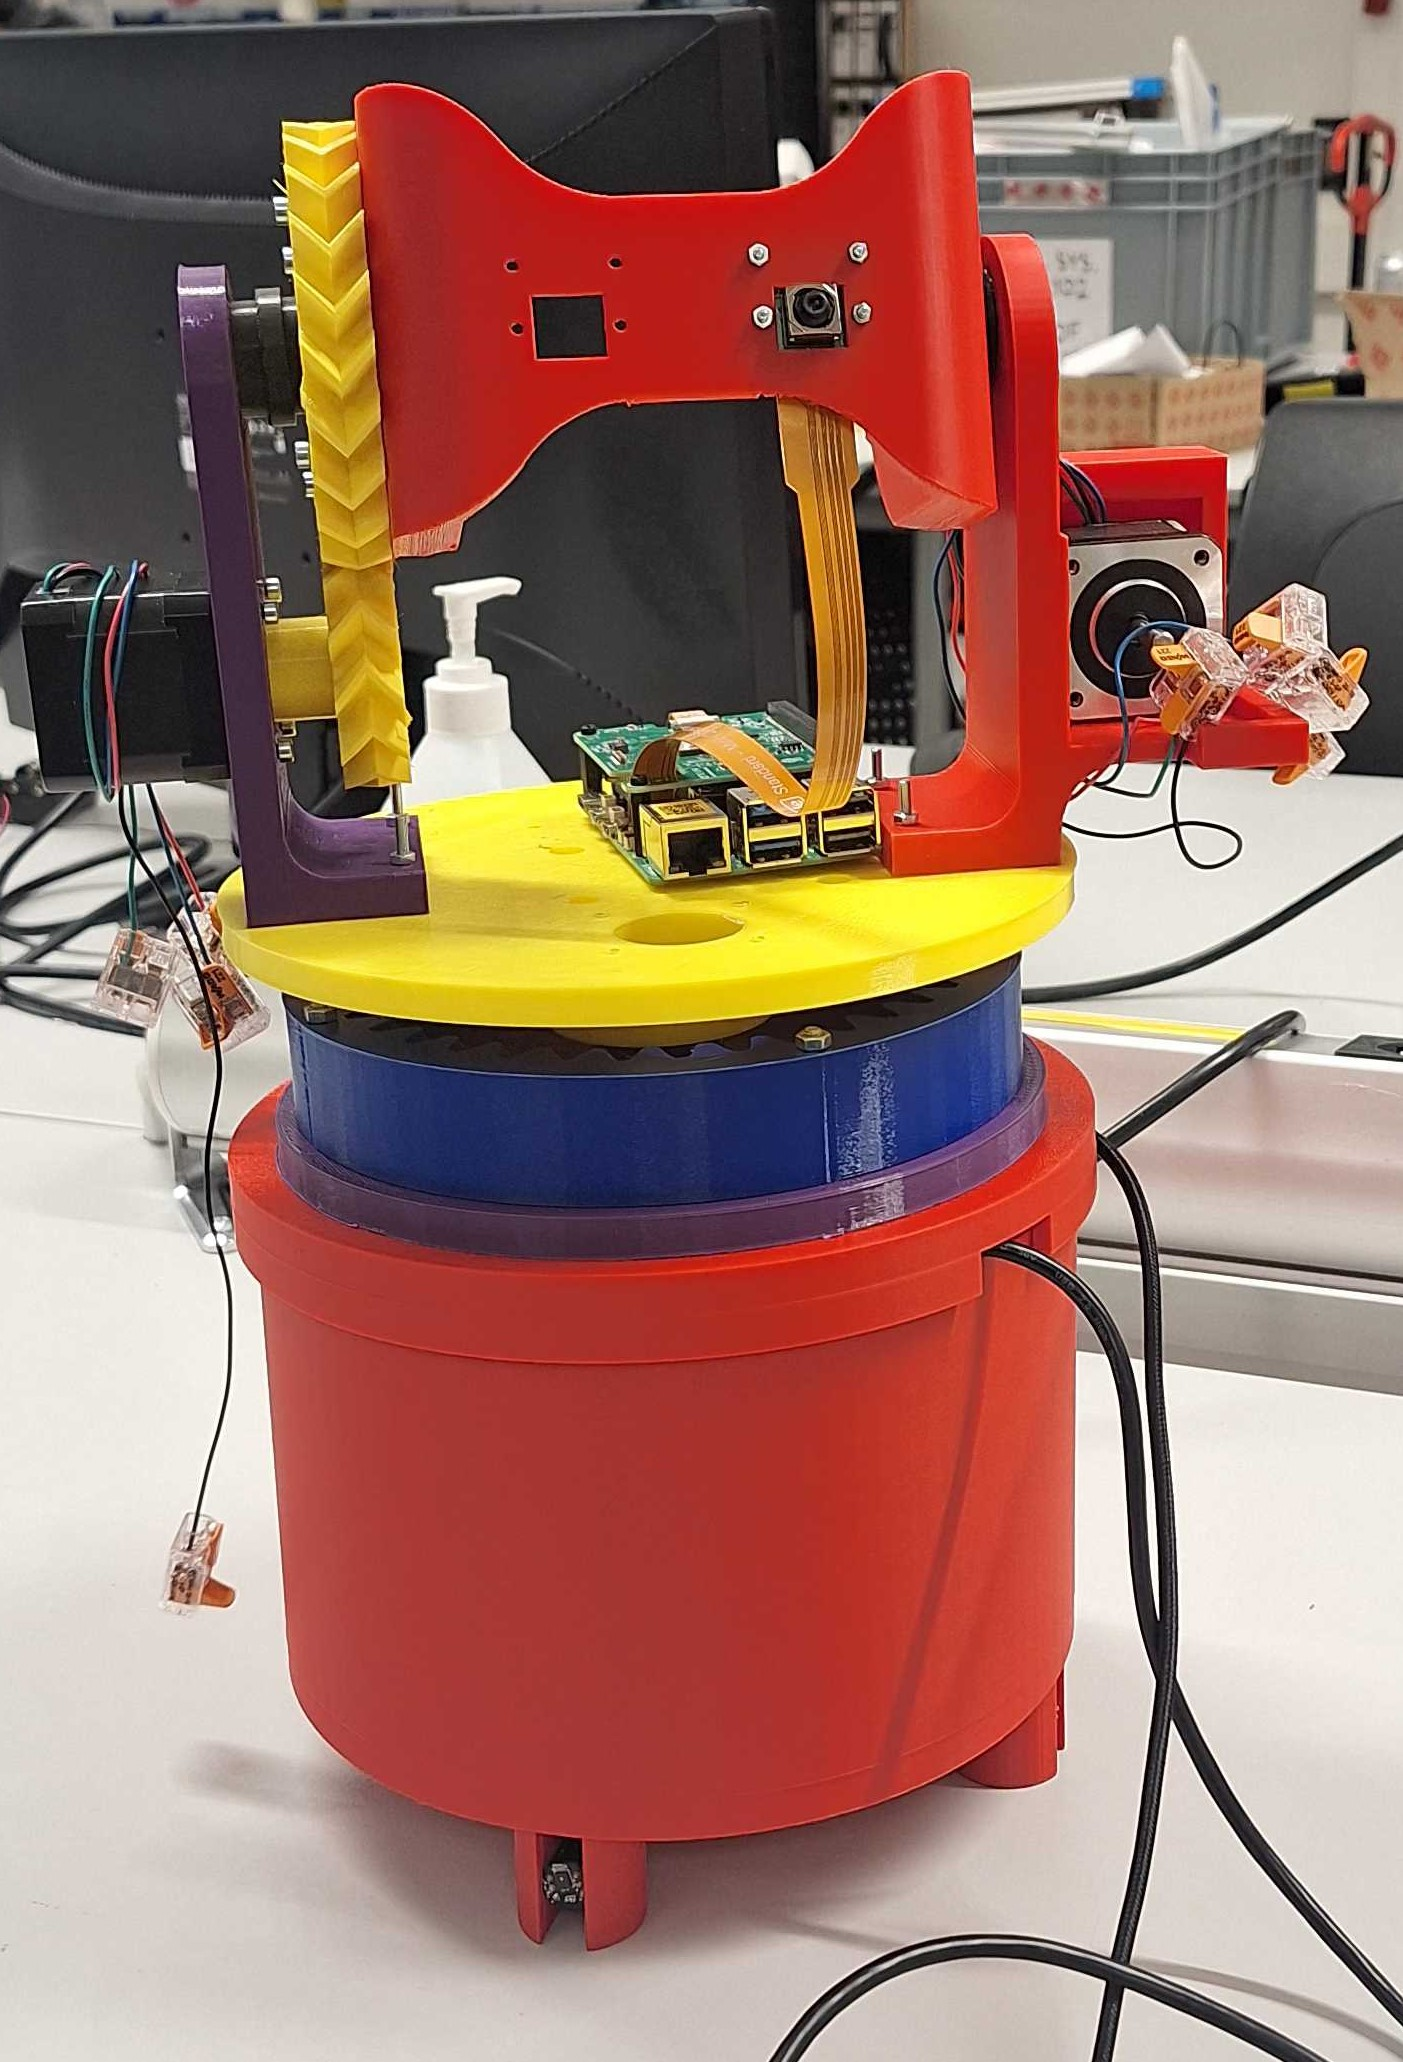
\includegraphics[width=0.5\linewidth]{Figures/Brage/FullSystem.jpg}
    \caption{Picture of the finished system}
    \label{fig:placeholder}
\end{figure}

\begin{figure}[H]
    \centering
    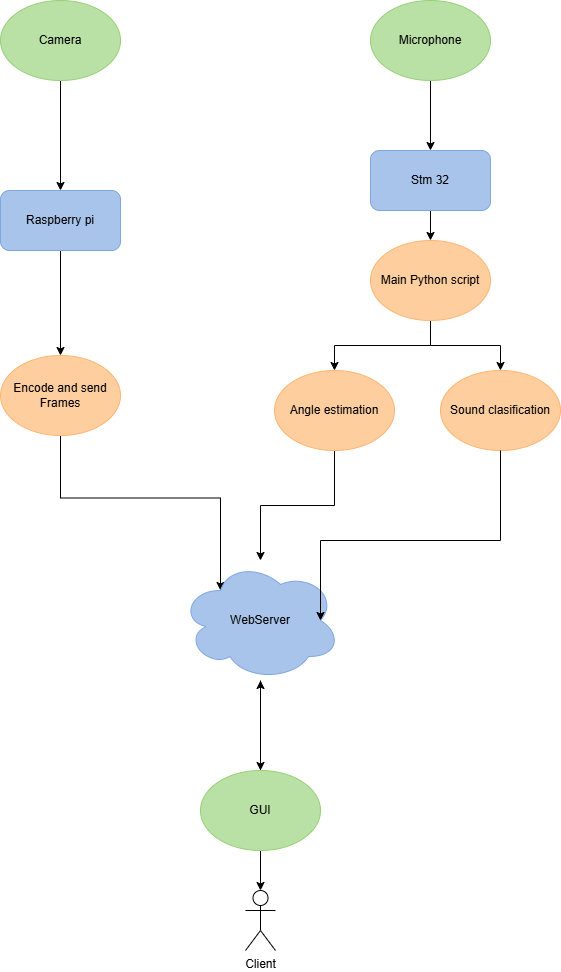
\includegraphics[width=0.5\linewidth]{Figures/Brage/FlowcahrtFullSystem.drawio.png}
    \caption{Low level flow chart of system}
    \label{fig:placeholder}
\end{figure}

\section{Sound signal acquisition results}
    \subsection{SAI acquisition test results}
    The SAI acquisition test resulted in the signal shown in Figure~\ref{fig:pcm_sai}.
    During the test, the azimuth estimation appeared random, which led to the troubleshooting of the acquisition pipeline. The troubleshooting results indicated, that the problem seamed to be related to data leakage or incorrect channel separation between the micropohones sharing the same line. This was supported by high correlation values between microphone pairs connected to the same line as shown in Figure~\ref{fig:corr_sai}. In addition, when one microphone from a pair was disconnected, the received signal still contained data in the channel representing the disconnected microphone. A more detailed explenation of this troubleshooting process is given in Section~\ref{sec:troubleshooting_sound_acquisition}.\\
    
    Despite the observed mixing between microphone channels, the signal was still sufficient to reconstruct understandable audio from the recording. The reconstructed WAV file contained a large amount of noise, but the speech produced by the student could still be understood. The signal was also still usable for MFCC extraction, althoguh Figure~\ref{fig:mel_spec_sai_test} shows that the speech-related spectral components were mixed with a considerable amount of high frequency noise. However, the signal quality was not sufficient for reliable DOA estimation, and additional filtering or correction would have beed required before using the signal for further analysis.

    \begin{figure}[h]
        \centering
        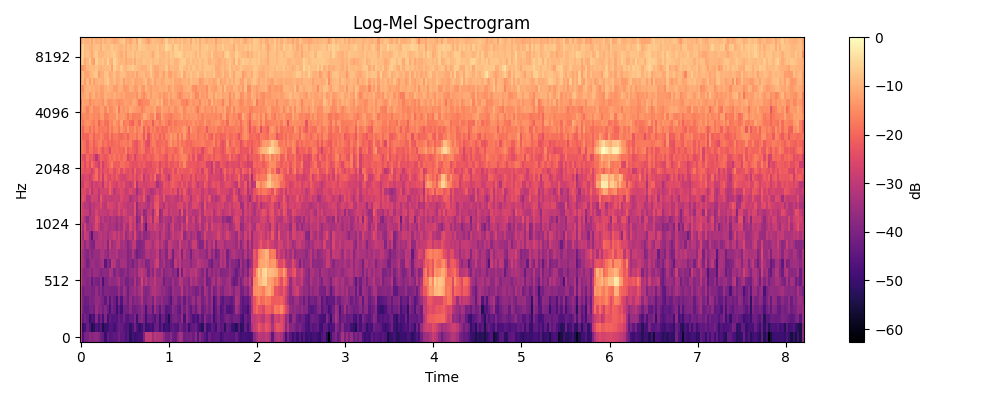
\includegraphics[width=1\linewidth]{Figures/mel-spec.png}
        \caption[Mel-spectrogram for SAI testing]{A Mel-spectrogram produced during the speech test using SAI}
        \label{fig:mel_spec_sai_test}
    \end{figure}
    
    \newpage
    \subsection{DFSDM acquisition test results}
    The resulting PCM signal acquired during the DFSDM test is shown in Figure~\ref{fig:pcm_dfsdm}. Compared with the SAI acquisition, the DFSDM signal appeared more stable and contained less visible noise. This was also reflected in the Mel-spectrogram shown in Figure~\ref{fig:mel_spec_dfsdm_test}, where the clapping-related frequency components were more clearly visible.\\

    The DFSDM signal also resulted in more consistent DOA estimation during the initial speech, and clapping-based tests. This with addition of the correlation matrix in Figure~\ref{fig:corr_dfsdm} indicates that the problem of data leakage has not occured. Based on these results, the DFSDM peripheral was selected as the final method for microphone data acquisition and was used in the lated tests involving recorded drone sound and the live drone.

\begin{figure}[h]
    \centering
    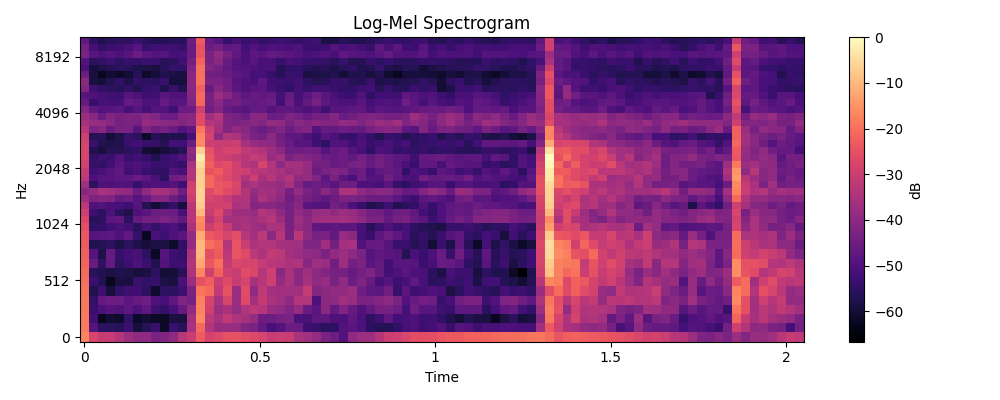
\includegraphics[width=1\linewidth]{Figures/Debug_mel_spectrogram1777801860.6435578.png}
    \caption[Mel-spectrogram for DFSDM testing]{A Mel-spectrogram produced during the clapping test using the DFSDM}
    \label{fig:mel_spec_dfsdm_test}
\end{figure}

\begin{figure}[H]
    \centering
    \begin{subfigure}[b]{0.48\textwidth}
        \centering
        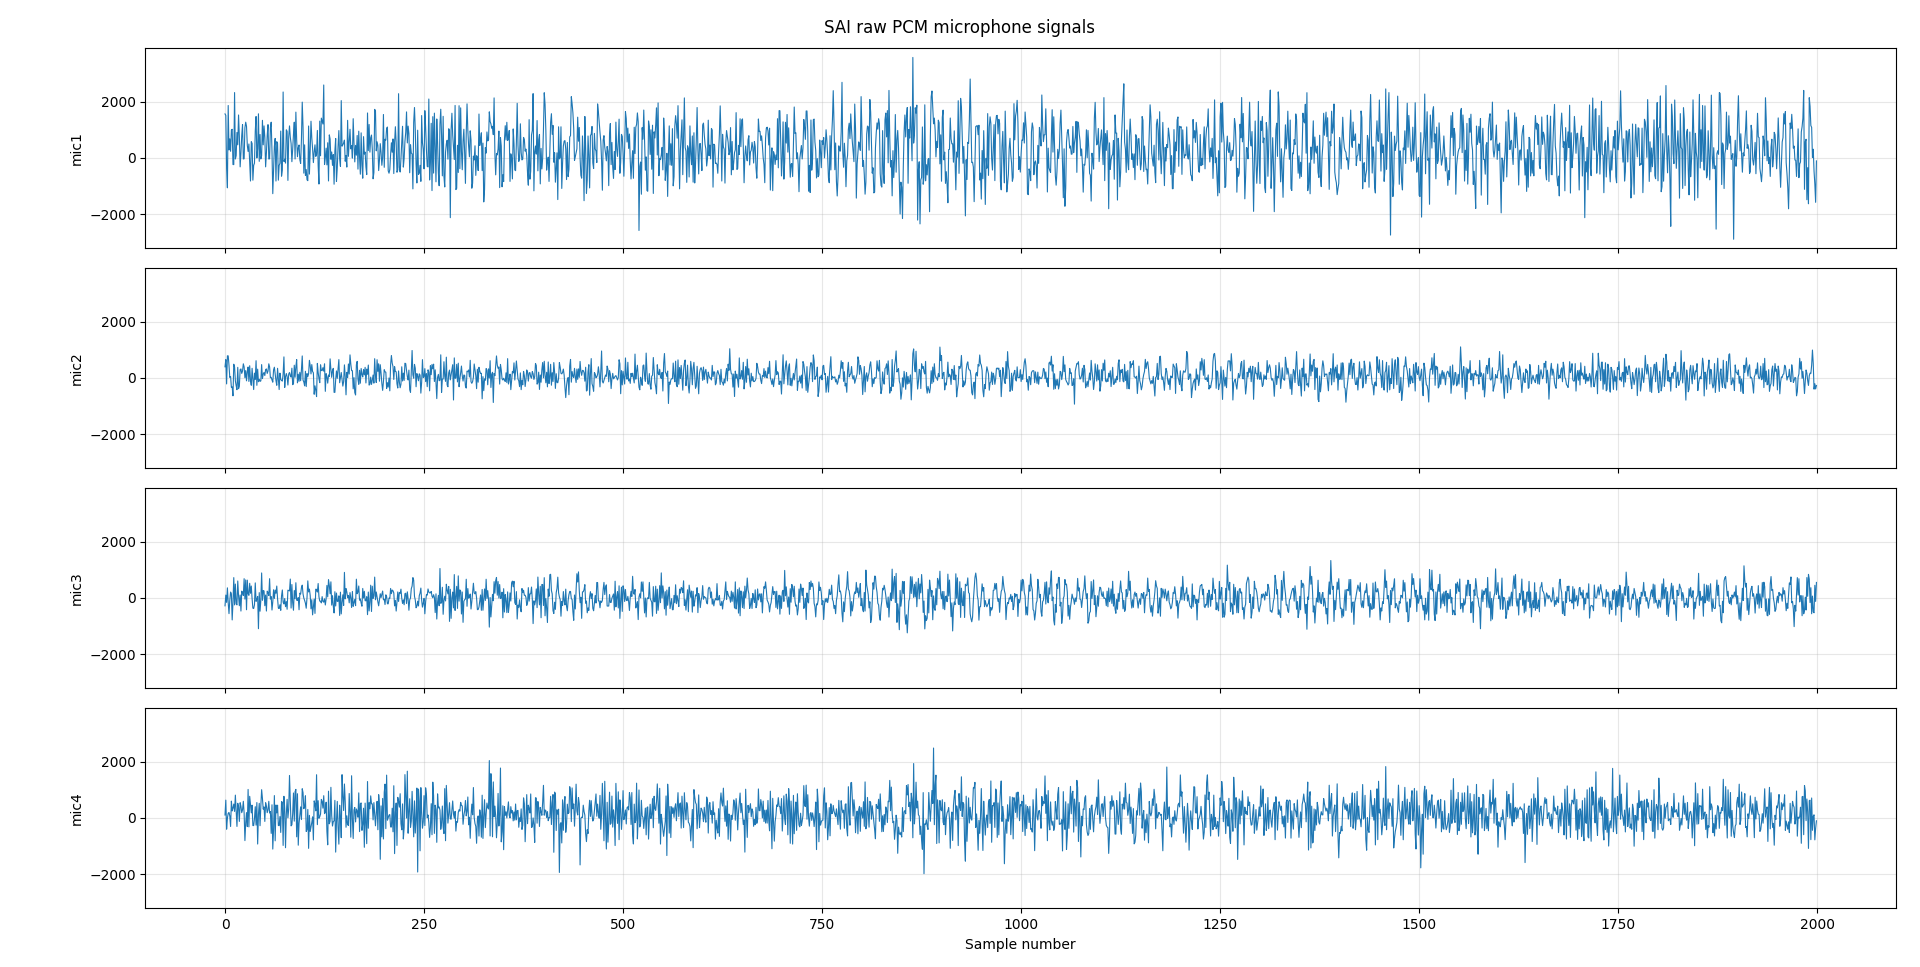
\includegraphics[width=\textwidth]{Figures/sai pcm figure.png}
        \caption[PCM when using the SAI]{PCM values transferred from MCU when acquiring PDM values through SAI }
        \label{fig:pcm_sai}
    \end{subfigure}
    \hfill
    \begin{subfigure}[b]{0.48\textwidth}
        \centering
        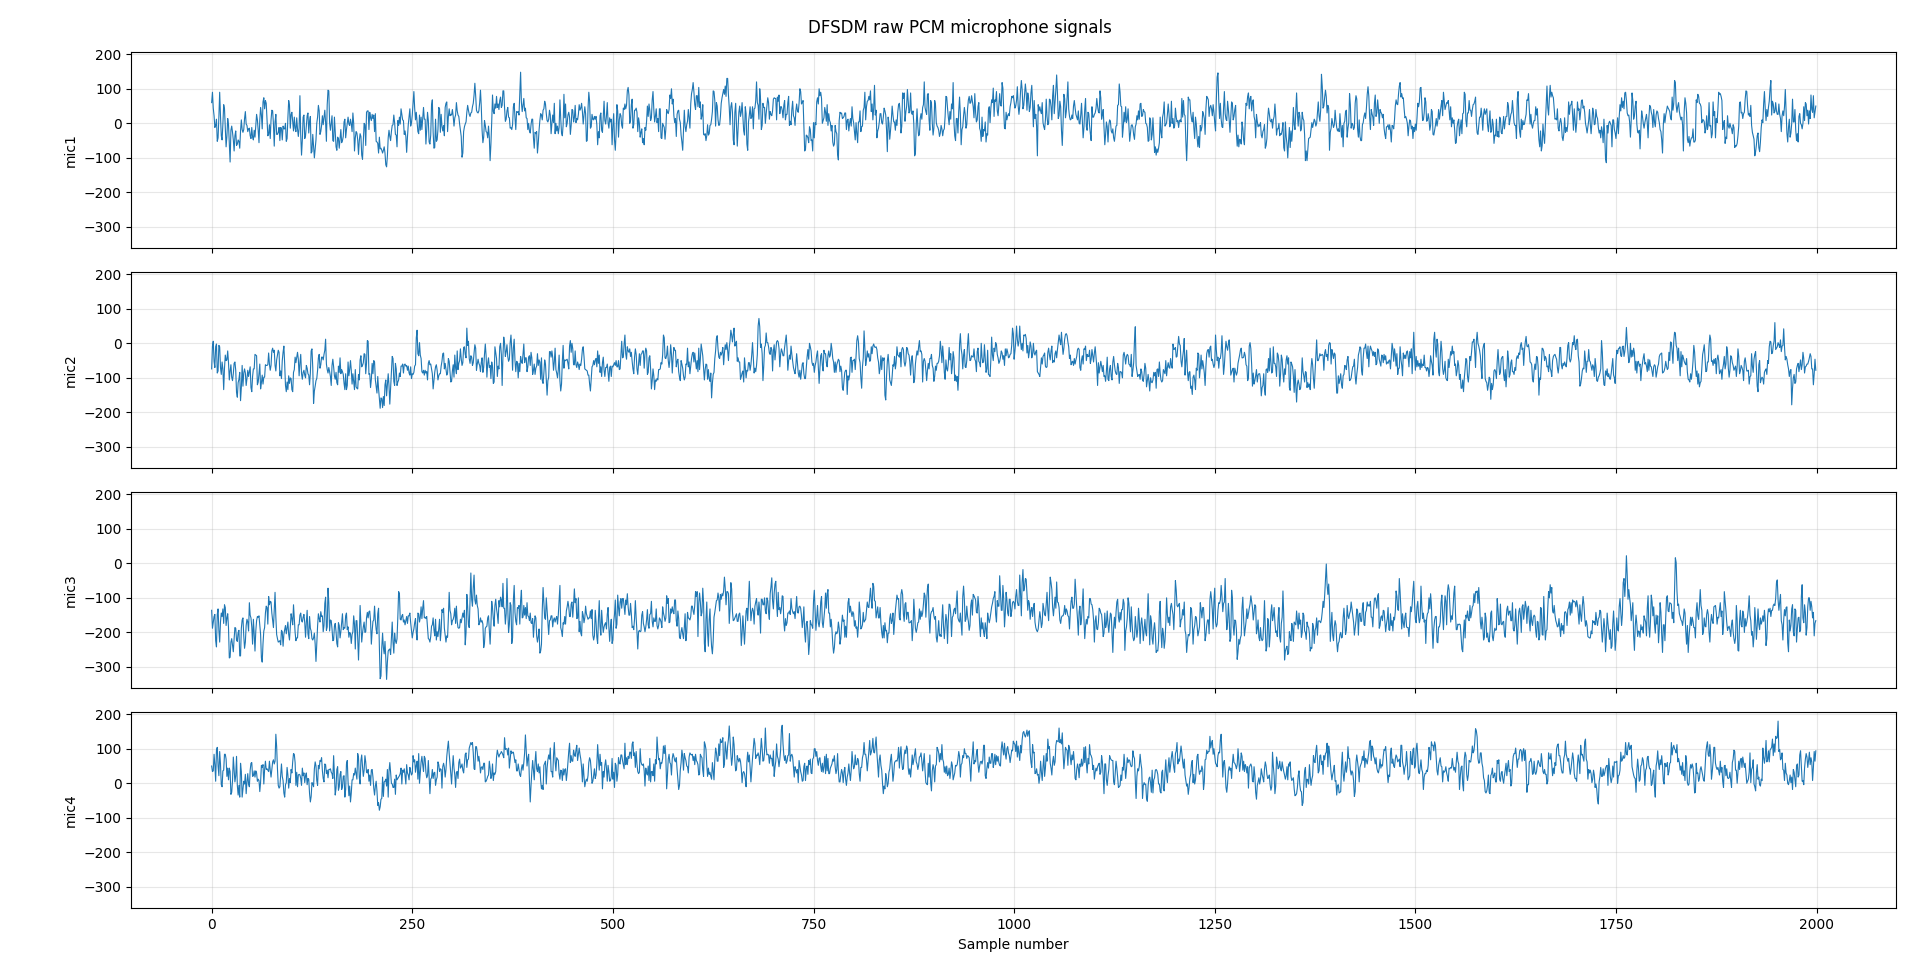
\includegraphics[width=\textwidth]{Figures/dfsdm pcm figure.png}
        \caption[PCM when using the DFSDM]{PCM values transferred from MCU when acquiring PDM values through DFSDM }
        \label{fig:pcm_dfsdm}
    \end{subfigure}
    \caption{Signals received by using the SAI amd DFSDM peripherals on STM32}
\label{fig:dfsdm_sai_signals}
\end{figure}

    \subsection{Comparison between SAI and DFSDM}
    As presented in the previous sections, the signals acquired using SAI and DFSDM differed considerably, even though the tests were performed with similair acoustic input signals. To quantify the difference between the two acquisition methods, the standard deviation was calculated for each microphone channel.\\
    
    The standard deviation was used to describe how much the measured PCM values deviated from the mean value of the signal. A higher standard deviation means that the samples vary more around the mean, which might indicate the presence of stocastic noise components in the signal, or the irregularity of the desired signal itself, assuming that the measured sound is similair between the tests. As shown in Figure~\ref{fig:std_sai_dfsdm}, the signal acquired using SAI had a significantly higher standard deviation than the signal acquired using DFSDM. Additionaly after the wav conversion has occured, it was clearly hearable that the DFSDM acquird signal contained much less noise. This supports the observation that the SAI signal contained larger irregular variations in the PCM values. \\
% move it? 
    The lower STD of the DFSDM signal is likely related to the internal filtering and decimation performed by the DFSDM peripheral. Unlike the SAI setup, the DFSDM peripheral converts the PDM stream to PCM using the configured sinc3 filter. This filter attenuates parts of the high-frequency components present in the signal before the PCM samples are produced. This likely contributed to the lower standard deviation observed in Figure~\ref{fig:std_sai_dfsdm}.\\

    \begin{figure}[h]
        \centering
        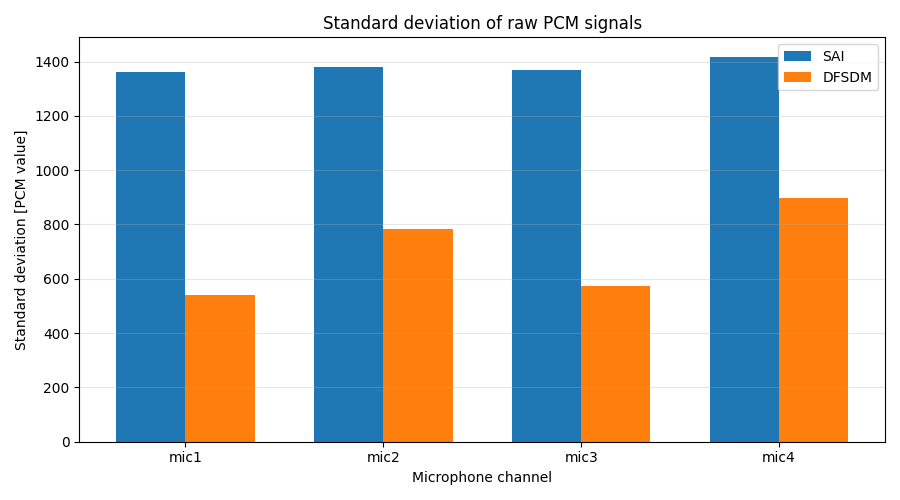
\includegraphics[width=0.5\linewidth]{Figures/std_sai_dfsdm.png}
        \caption[Std comparison of SAI and DFSDM]{Std of the signals gathered with SAI and DFSDM}
        \label{fig:std_sai_dfsdm}
    \end{figure}
    
\begin{figure}[H]
    \centering
    \begin{subfigure}[b]{0.48\textwidth}
        \centering
        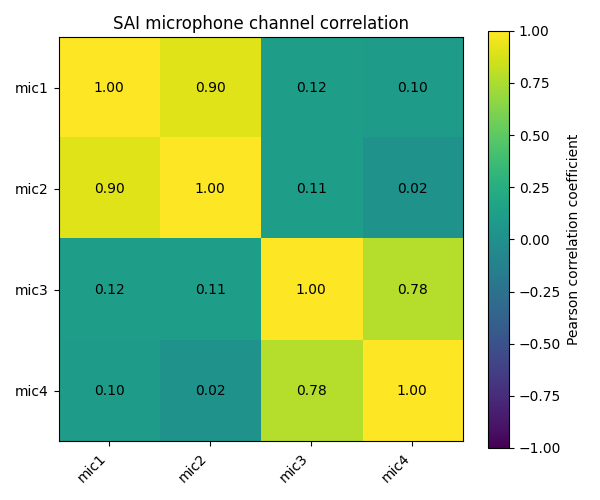
\includegraphics[width=\textwidth]{Figures/sai_correlation_matrix.png}
        \caption[Signal correlation for the SAI]{Signal correlation matrix between each microphone pair using the SAI}
        \label{fig:corr_sai}
    \end{subfigure}
    \hfill
    \begin{subfigure}[b]{0.48\textwidth}
        \centering
        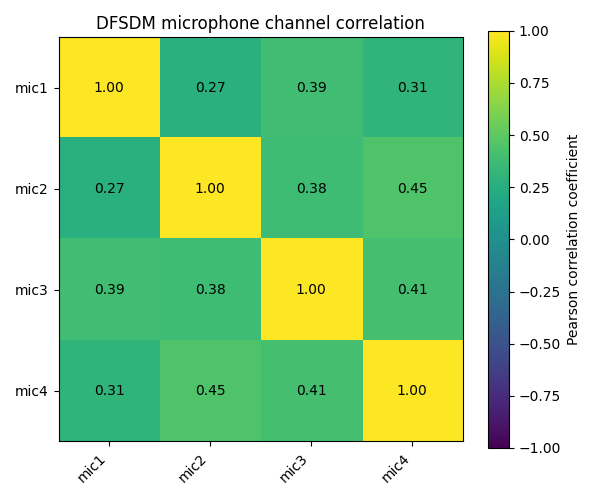
\includegraphics[width=\textwidth]{Figures/dfsdm_correlation_matrix.png}
        \caption[Signal correlation for the DFSDM]{Signal correlation matrix between each microphone pair using the DFSDM}
        \label{fig:corr_dfsdm}
    \end{subfigure}
    \caption{Comparison between the microphone pair correlations using SAI and DFSDM for sound acquisition}
\label{fig:corr_comparison}
\end{figure}

\newpage
    \subsection{DC offset removal}
    The results of the DC offset removal can be seen in Figure~\ref{fig:dc_offset_dfsdm}. As expected, the values were centered around zero.

    \begin{figure}[h]
        \centering
        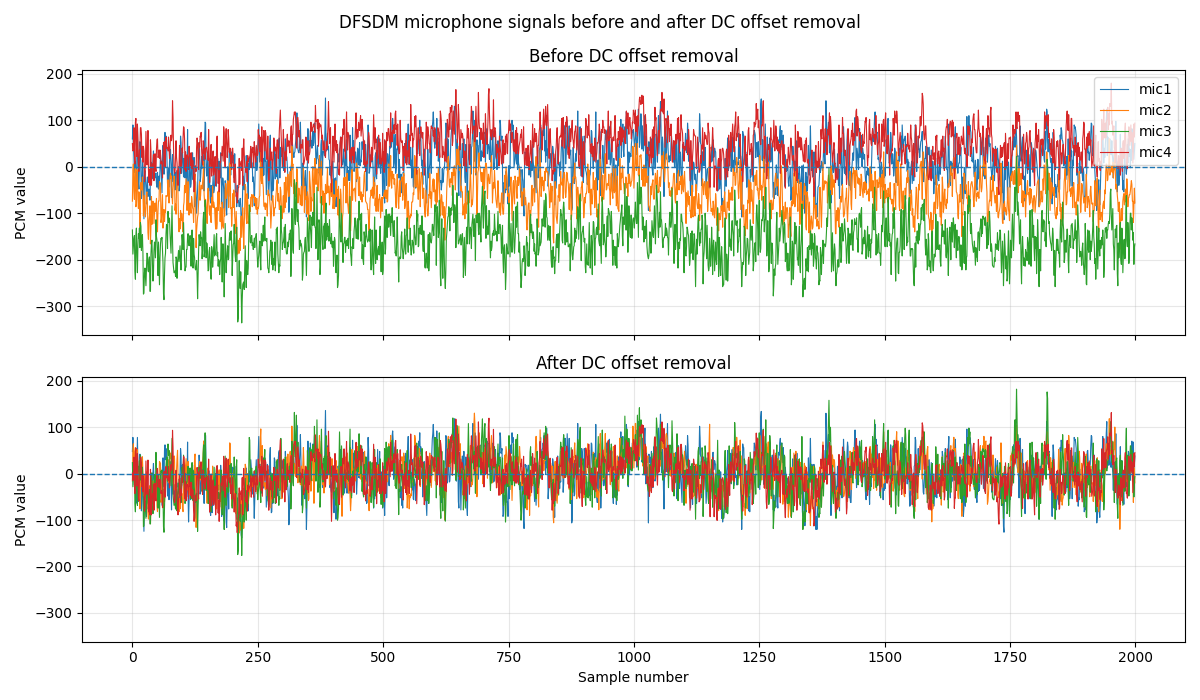
\includegraphics[width=0.65\linewidth]{Figures/DC_offset for dfsdm.png}
        \caption{Results of the DC offset for the microphone signal}
        \label{fig:dc_offset_dfsdm}
    \end{figure}
    
\section{DOA estimation testing results}
The DOA estimation results are presented in three stages: human-generated sounds, recorded drone-like sounds, and live-drone testing.

\subsection{Results of the first DOA testing stage}
In the empty classroom, the DOA estimate pointed close to the expected source direction when the student was positioned at approximately 90 degrees, as shown in Figure~\ref{fig:DOA_estimation_first_stage}.

\begin{figure}[h]
    \centering
    %\begin{subfigure}[b]{0.48\linewidth}
    %    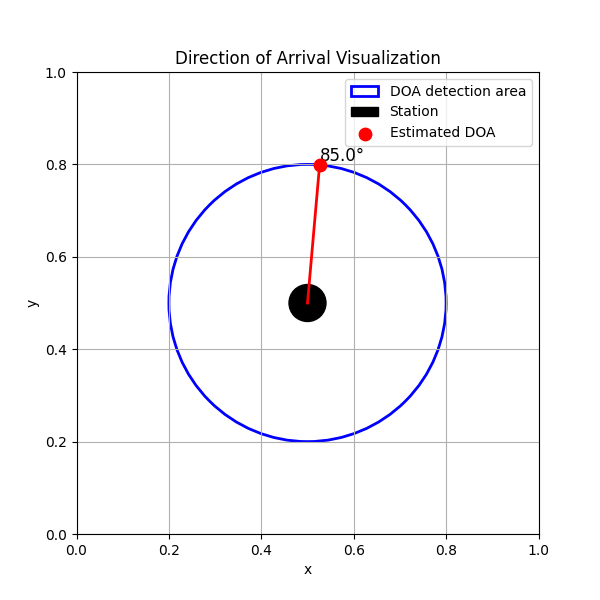
\includegraphics[width=\linewidth]{Figures/Debug_doa_estimation1777722708.9166152.png}
    %    \caption{First stage estimation nr.1 (empty classroom)}
    %    \label{fig:f_stage_est_1}
    %\end{subfigure}
    %\hfill
    %\begin{subfigure}[b]{0.48\linewidth}
    %    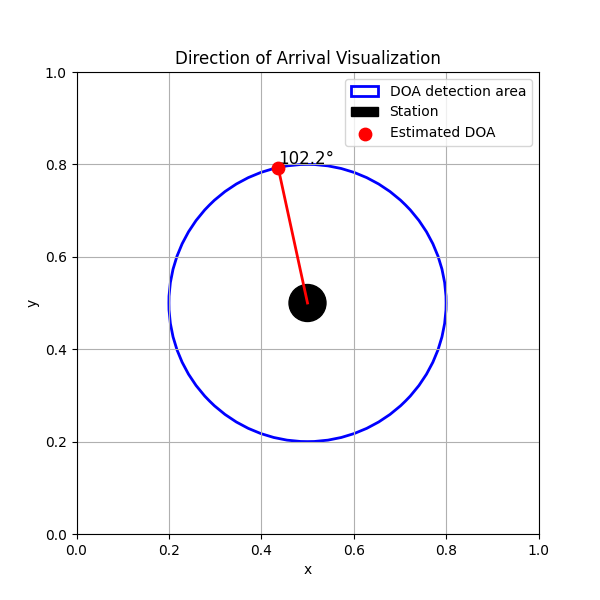
\includegraphics[width=\linewidth]{Figures/Debug_doa_estimation1777722714.2824512.png}
    %    \caption{First stage estimation nr.2 (empty classroom)}
    %    \label{fig:f_stage_est_1}
    %\end{subfigure}
    %\hfill
    \begin{subfigure}[b]{0.3\linewidth}
        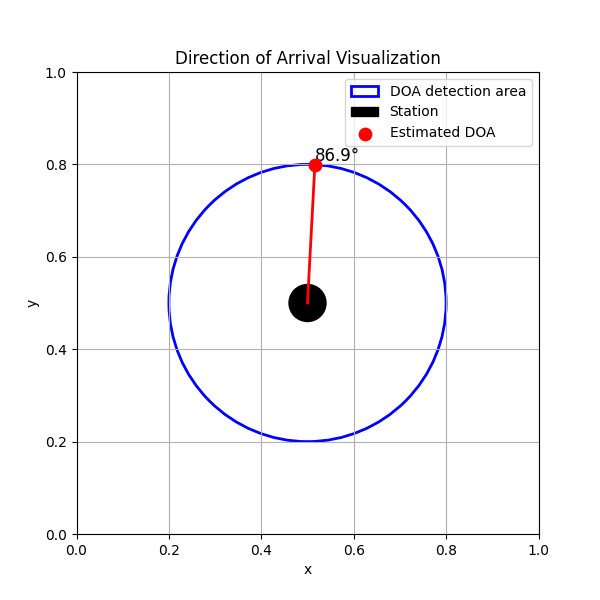
\includegraphics[width=\linewidth]{Figures/Debug_doa_estimation1777722716.9580076.png}
        \caption{First stage estimation nr.3 (empty classroom)}
        \label{fig:f_stage_est_1}
    \end{subfigure}
    \hfill
    \begin{subfigure}[b]{0.3\linewidth}
        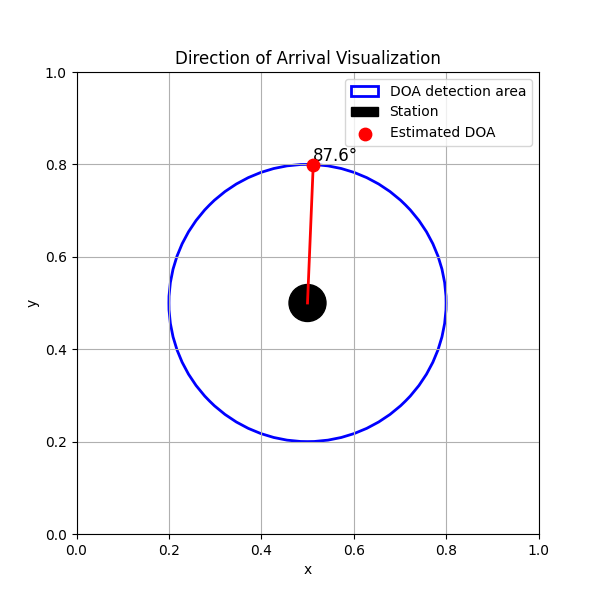
\includegraphics[width=\linewidth]{Figures/Debug_doa_estimation1777722719.6664054.png}
        \caption{First stage estimation nr.4 (empty classroom)}
        \label{fig:f_stage_est_1_2}
    \end{subfigure}
    \hfill
    \caption{DOA estimation for the first testing stage, with an empty calssroom}
    \label{fig:DOA_estimation_first_stage}
\end{figure}
\newpage

However in the occupied classroom, the results changed significantly. The DOA estimate no longer pointed consistently towards the intended test sound. Instead, the estimated direction was often towards a group of students talking in the room at angle of approximately 45 degrees from the system, as seen in Figure~\ref{fig:DOA_estimation_first_stage_full_class}. This proves that the DOA module estimated the direction of the dominant sound source rather than the desired test sound source. 

\begin{figure}[h]
    \centering
    \begin{subfigure}[b]{0.48\linewidth}
        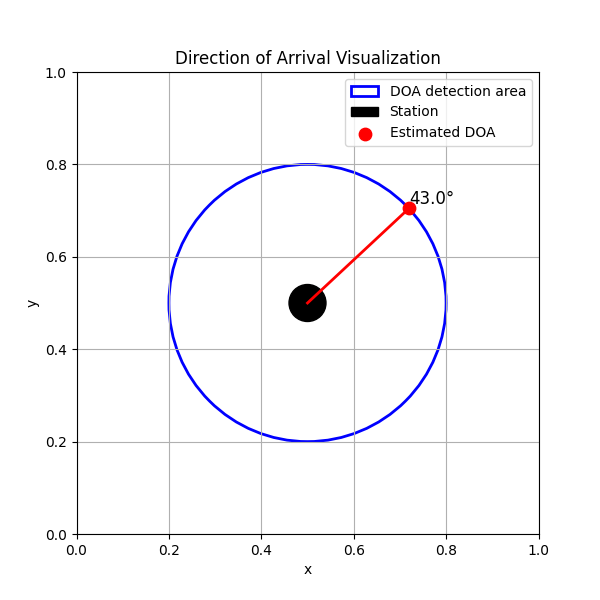
\includegraphics[width=\linewidth]{Figures/Debug_doa_estimation1777723161.8334353.png}
        \caption{First stage estimation nr.1 (full classroom)}
        \label{fig:f_stage_est_1_f}
    \end{subfigure}
    \hfill
    \begin{subfigure}[b]{0.48\linewidth}
        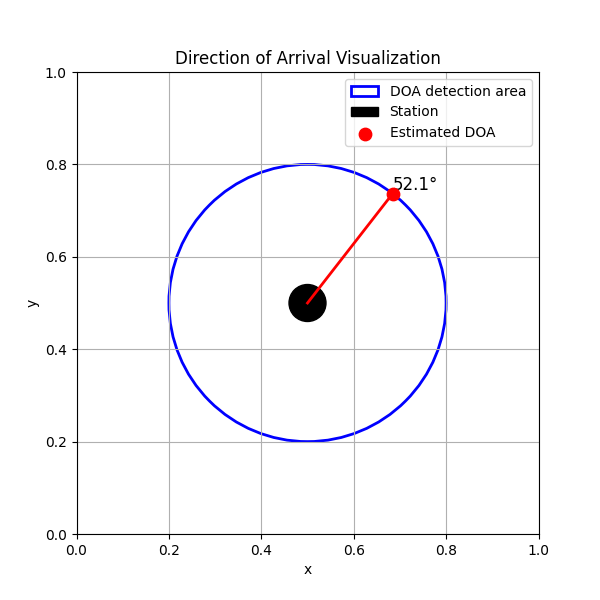
\includegraphics[width=\linewidth]{Figures/Debug_doa_estimation1777723163.390828- VIKTIG 2.png}
        \caption{First stage estimation nr.2 (full classroom)}
        \label{fig:f_stage_est_2_f}
    \end{subfigure}
   % \hfill
   % \begin{subfigure}[b]{0.48\linewidth}
   %     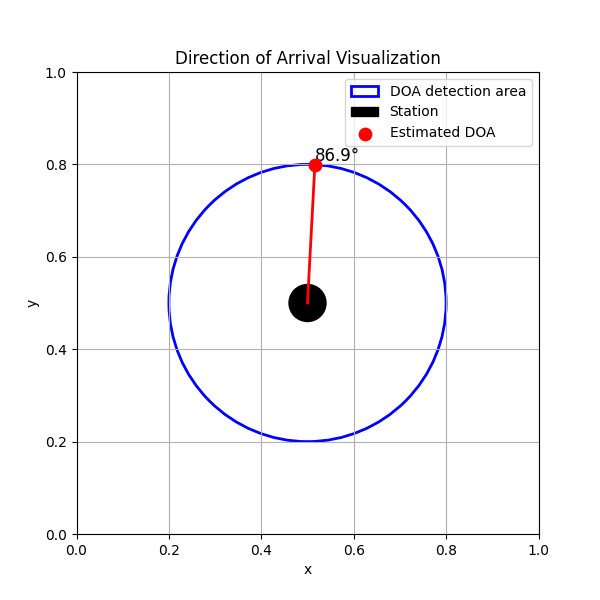
\includegraphics[width=\linewidth]{Figures/Debug_doa_estimation1777722716.9580076.png}
   %     \caption{First stage estimation nr.3 (full classroom)}
   %     \label{fig:f_stage_est_3_f}
   % \end{subfigure}
   % \hfill
   % \begin{subfigure}[b]{0.48\linewidth}
    %    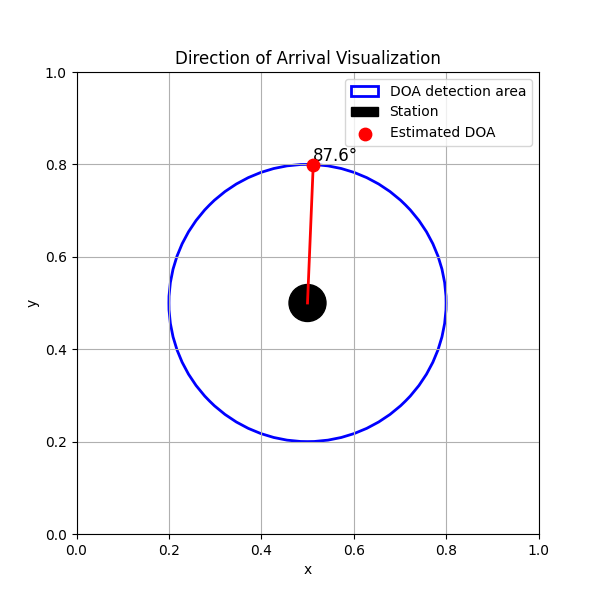
\includegraphics[width=\linewidth]{Figures/Debug_doa_estimation1777722719.6664054.png}
   %     \caption{First stage estimation nr.4 (full classroom)}
   %     \label{fig:f_stage_est_4_f}
   % \end{subfigure}
    \hfill
    \caption{DOA estimation for the first testing stage, with a full calssroom}
    \label{fig:DOA_estimation_first_stage_full_class}
\end{figure}

These results supported the need for a classification stage before the DOA result is interpreted as a drone direction. Without such classification, the DOA module may estimate the direction of other dominant sounds in the environment. 
\newpage
\subsection{The second DOA testing stage}
The DC motor test did not produce reliable DOA estimates at distances above a few centimeters. The system was unable to detect the DC-motor, which resulted in random DOA estimation. When the DC-motor was being hold around 30 cm away from the microphone platform, the DOA estimation was as accurate as for the human sound on the distance of few meters. The frequency bands present in the signal, can be seen in Figure~\ref{fig:dc_motor_mel}. 

\begin{figure}[h]
    \centering
    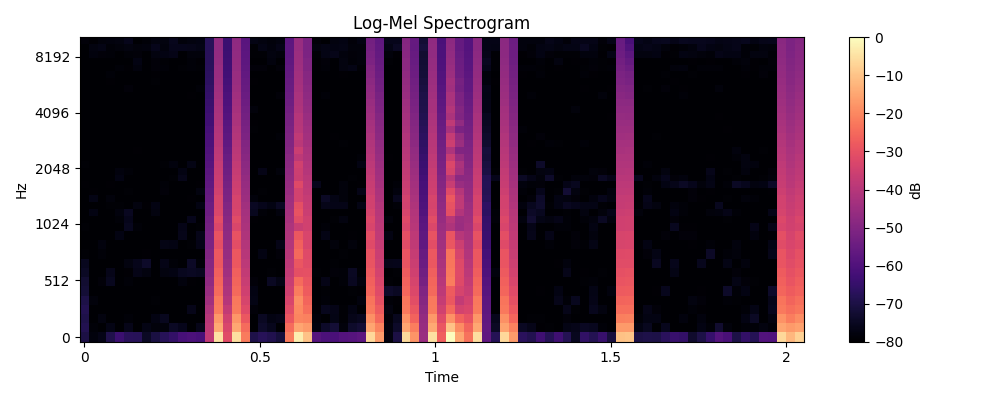
\includegraphics[width=0.5\linewidth]{Figures/Debug_mel_spectrogram1777801048.636684.png}
    \caption[DC-motor Mel-spectrogram]{The components present in the acoustic signal produced by the DC-motor}
    \label{fig:dc_motor_mel}
\end{figure}

The next test, was conducted by using the drone sound from the video, which resulted in a consistent and accurate DOA estimation on the testing distance, as can be seen in Figure~\ref{fig:DOA_estimation_second_stage}. The frequency bands present in the signal are shown in Figure~\ref{fig:mel_specs}.       

\begin{figure}[h]
    \centering
    \begin{subfigure}[b]{0.4\linewidth}
        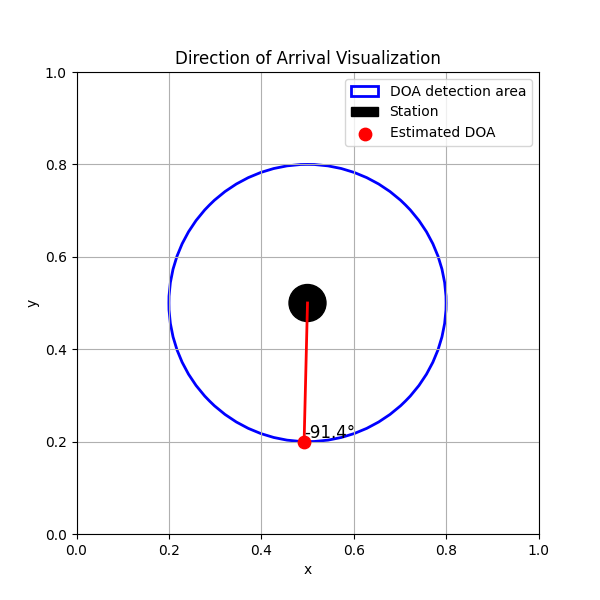
\includegraphics[width=\linewidth]{Figures/Debug_doa_estimation1777801847.8342373.png}
        \caption{Second stage estimation nr.1}
        \label{fig:f_stage_est_1_f}
    \end{subfigure}
    \hfill
    \begin{subfigure}[b]{0.4\linewidth}
        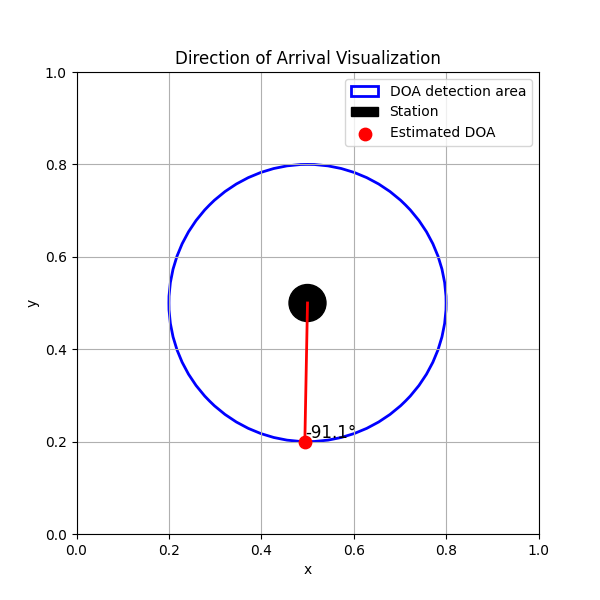
\includegraphics[width=\linewidth]{Figures/Debug_doa_estimation1777801851.314917.png}
        \caption{Second stage estimation nr.2}
        \label{fig:f_stage_est_2_f}
    \end{subfigure}
    \hfill
    \caption{DOA estimation for the second testing stage using the drone video}
    \label{fig:DOA_estimation_second_stage}
\end{figure}
\newpage
\begin{figure}[h]
    \centering
    \begin{subfigure}[b]{0.4\linewidth}
        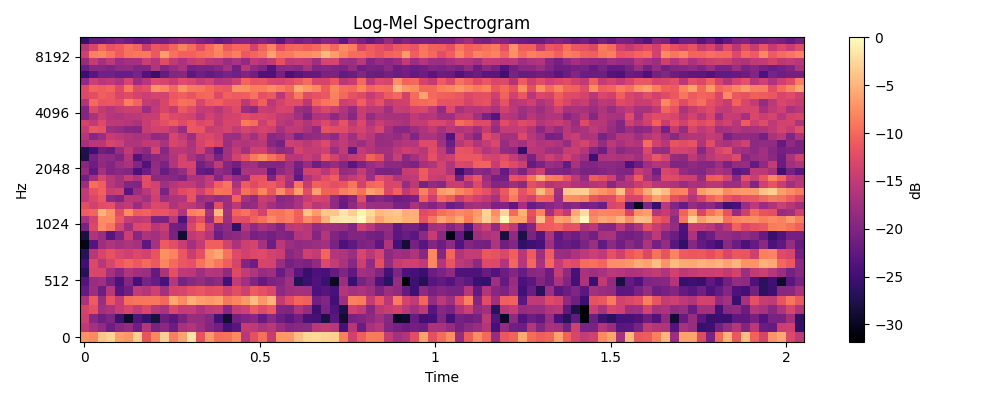
\includegraphics[width=\linewidth]{Figures/Debug_mel_spectrogram1777801847.8342373.png}
        \caption{Mel-spectrogram from the second stage DOA testing nr.1}
        \label{fig:mel_spec_1}
    \end{subfigure}
    \hfill
    \begin{subfigure}[b]{0.4\linewidth}
        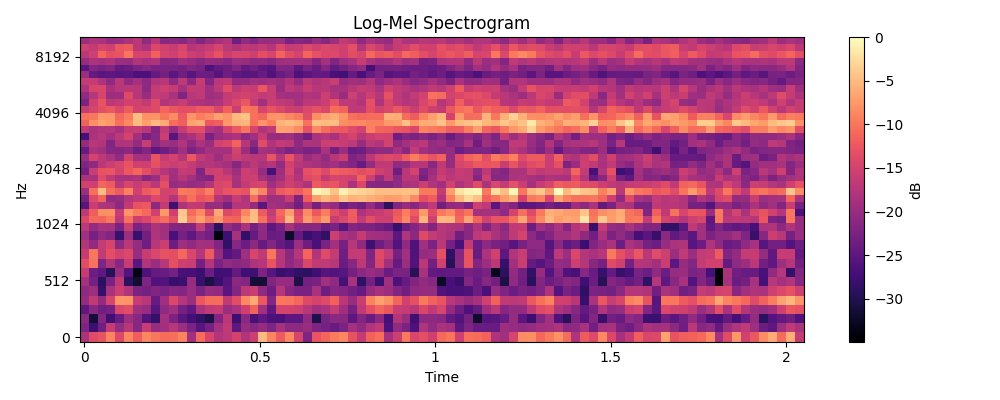
\includegraphics[width=\linewidth]{Figures/Debug_mel_spectrogram1777801851.314917.png}
        \caption{Mel-spectrogram from the second stage DOA testing nr.2}
        \label{fig:mel_spec_2}
    \end{subfigure}
    \hfill
    \caption{Mel-spectrograms produced during the second stage of DOA testing}
    \label{fig:mel_specs}
\end{figure}

The results of the test invloving the sound volume of around 50\% were mixed, as the drone signal was for the most part not recorded by the system, which resulted in less reliable DOA estimation.\\

The last test where the sound was reduced to around 5\% resulted in complete lack of drone detection, which resulted in random DOA estimation.\\

Since the drone sound was for the most part not detected, when using the phone volume of 50\% and 5\%, the received signals were compared by calculating the RMS values across the microphone channels after the DC offset removal. The 100\% phone volume test, had the highest received PCM level, while the 50\% and 5\% volume tests were approximately 9db lower as seen in Figure~\ref{fig:rms_phone_volumes}. However the 50\% and 5\% tests have produced quite similair RMS values, which may indicate that both signals were strongly influenced by the background noise. 

\begin{figure}[h]
    \centering
    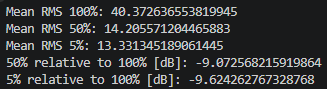
\includegraphics[width=0.5\linewidth]{Figures/image.png}
    \caption{The RMS values for the drone sound produced by the phone of varying volume levels}
    \label{fig:rms_phone_volumes}
\end{figure}

The second stage of the DOA testing, has proven that the system is capable of detecting the drone, if the sound produced by it is loud enough.\\

\subsection{The third DOA testing stage}
The result of the first no drone present test, conducted to measure the noise level in the laboratory was saved as the  Mel-spectrogram is shown in Figure~\ref{fig:stage_3_noise_present_no_drone}. Since the ML classification was not applied during the baseline test, the DOA module could still estimate the sound direction based on the dominant background noise, which proved again, that the ML has to be applied for the system to correctly estimate the DOA of the incoming drone.\\

\begin{figure}[h]
    \centering
    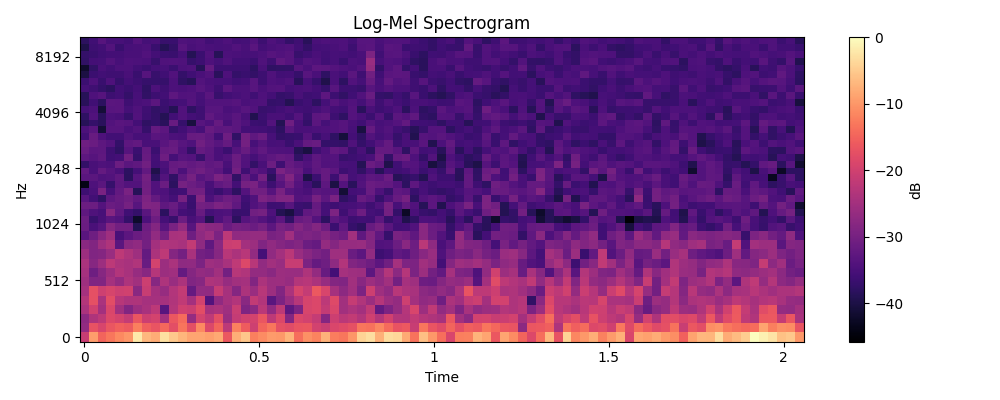
\includegraphics[width=0.5\linewidth]{Figures/Debug_mel_spectrogram1777882767.382446.png}
    \caption{Noisy frequency bands}
    \label{fig:stage_3_noise_present_no_drone}
\end{figure}
\newpage

The next test involving the use of the live-drone, which was circulating around the tower has resulted in the DOA estimation seen in Figure~\ref{fig:3_stage_no_camera-doa} and the following Mel-spectrogram seen in Figure~\ref{fig:mel_spec_present}. The resulting DOA estimation was quite accuarate, and the final test involving the ML and camera could be conducted.  \\

\begin{figure}[h]
    \centering
    \begin{subfigure}[b]{0.5\linewidth}
        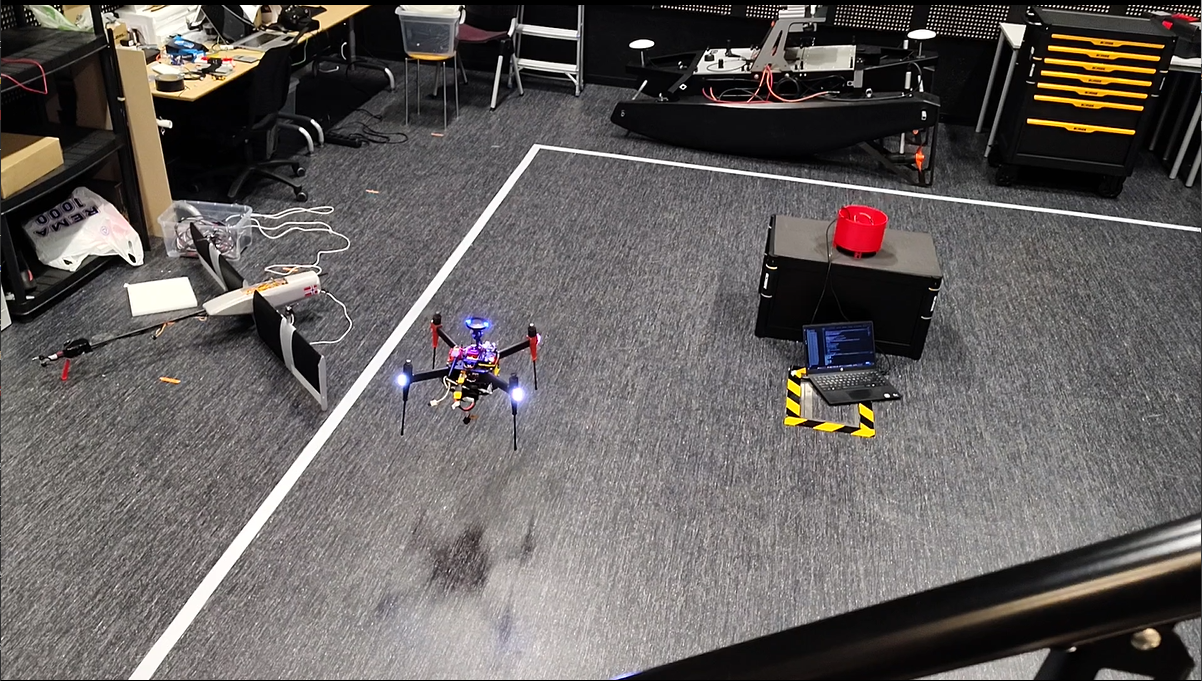
\includegraphics[width=\linewidth]{Figures/test_doa_no_camera.png}
    \caption{The actual drone position}
    \label{fig:picture_drone_position}
    \end{subfigure}
    \hfill
    %\vspace{2em}
    \begin{subfigure}[b]{0.40\linewidth}
        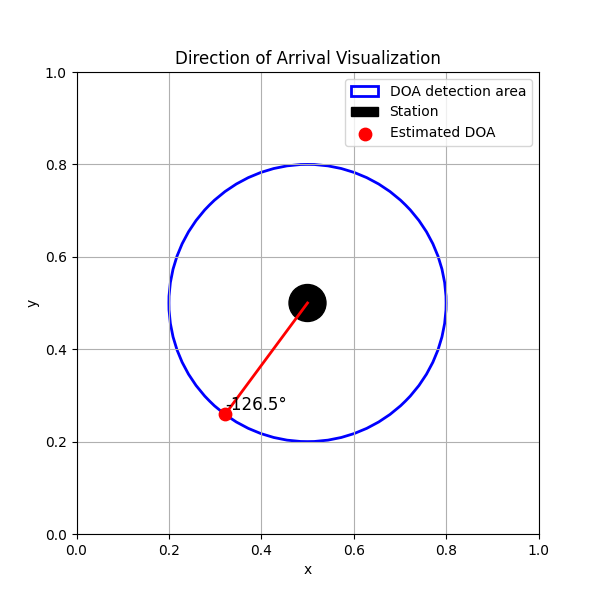
\includegraphics[width=\linewidth]{Figures/Debug_doa_estimation1777884326.4922612.png}
    \caption{The estimated DOA of the drone present}
    \label{fig:doa_estimation_3_stage_no_camera}
    \end{subfigure}
    \hfill
    \begin{subfigure}[b]{0.5\linewidth}
        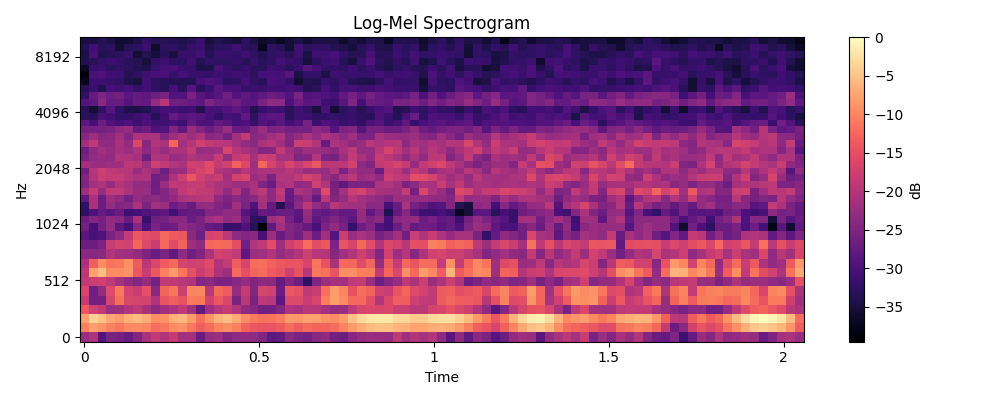
\includegraphics[width=1\linewidth]{Figures/Debug_mel_spectrogram1777884268.2983675.png}
    \caption{Mel-spectrogram for the drone present}
    \label{fig:mel_spec_present}
    \end{subfigure}
    \hfill
    \caption{The first DOA estimation using the live-drone, without the ML or the camera}
    \label{fig:3_stage_no_camera-doa}
\end{figure}
  

The results of the final DOA test, where ML and camera was implemented, can be seen in Figure~\ref{fig:doa_screenshots}.\\

\begin{figure}[H]
    \centering
    \begin{subfigure}[b]{0.48\linewidth}
        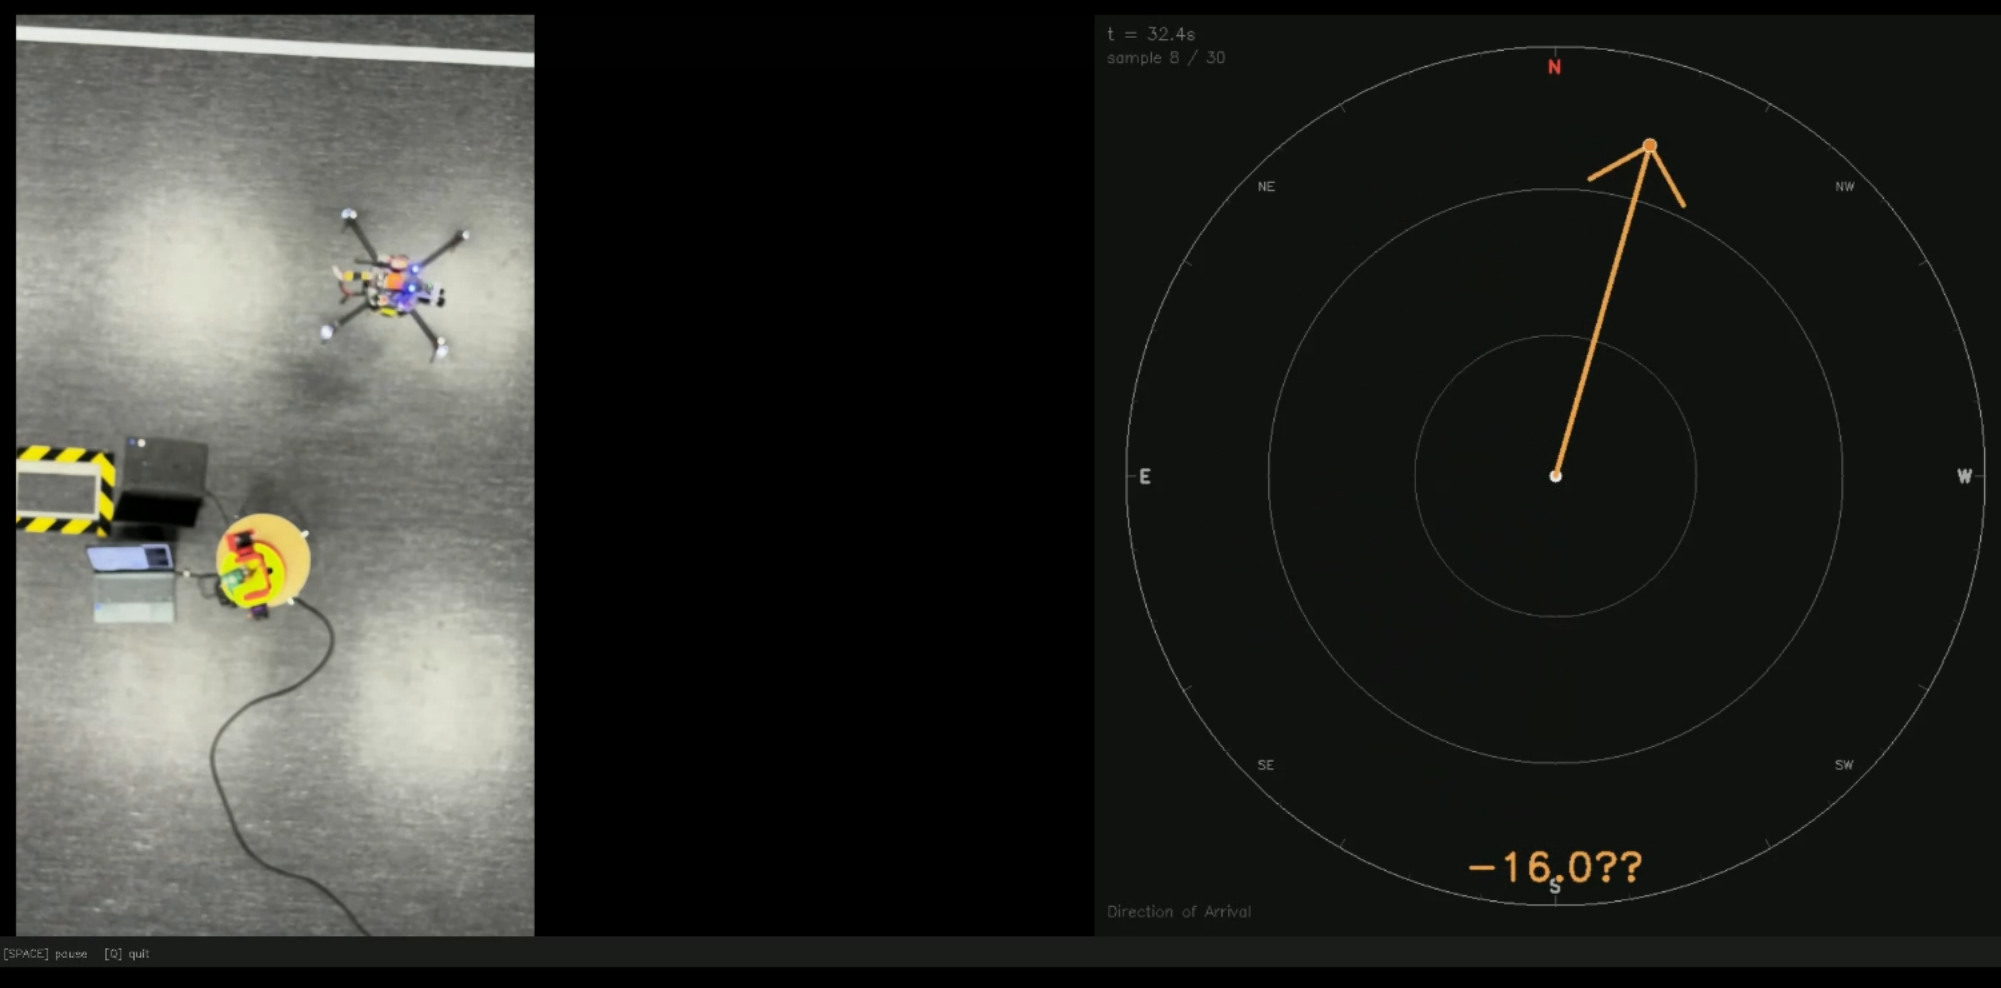
\includegraphics[width=\linewidth]{Figures/Andreas/DOA_estimation/Drone_DOA_1.png}
        \caption{}
        \label{fig:doa1}
    \end{subfigure}
    \hfill
    \begin{subfigure}[b]{0.48\linewidth}
        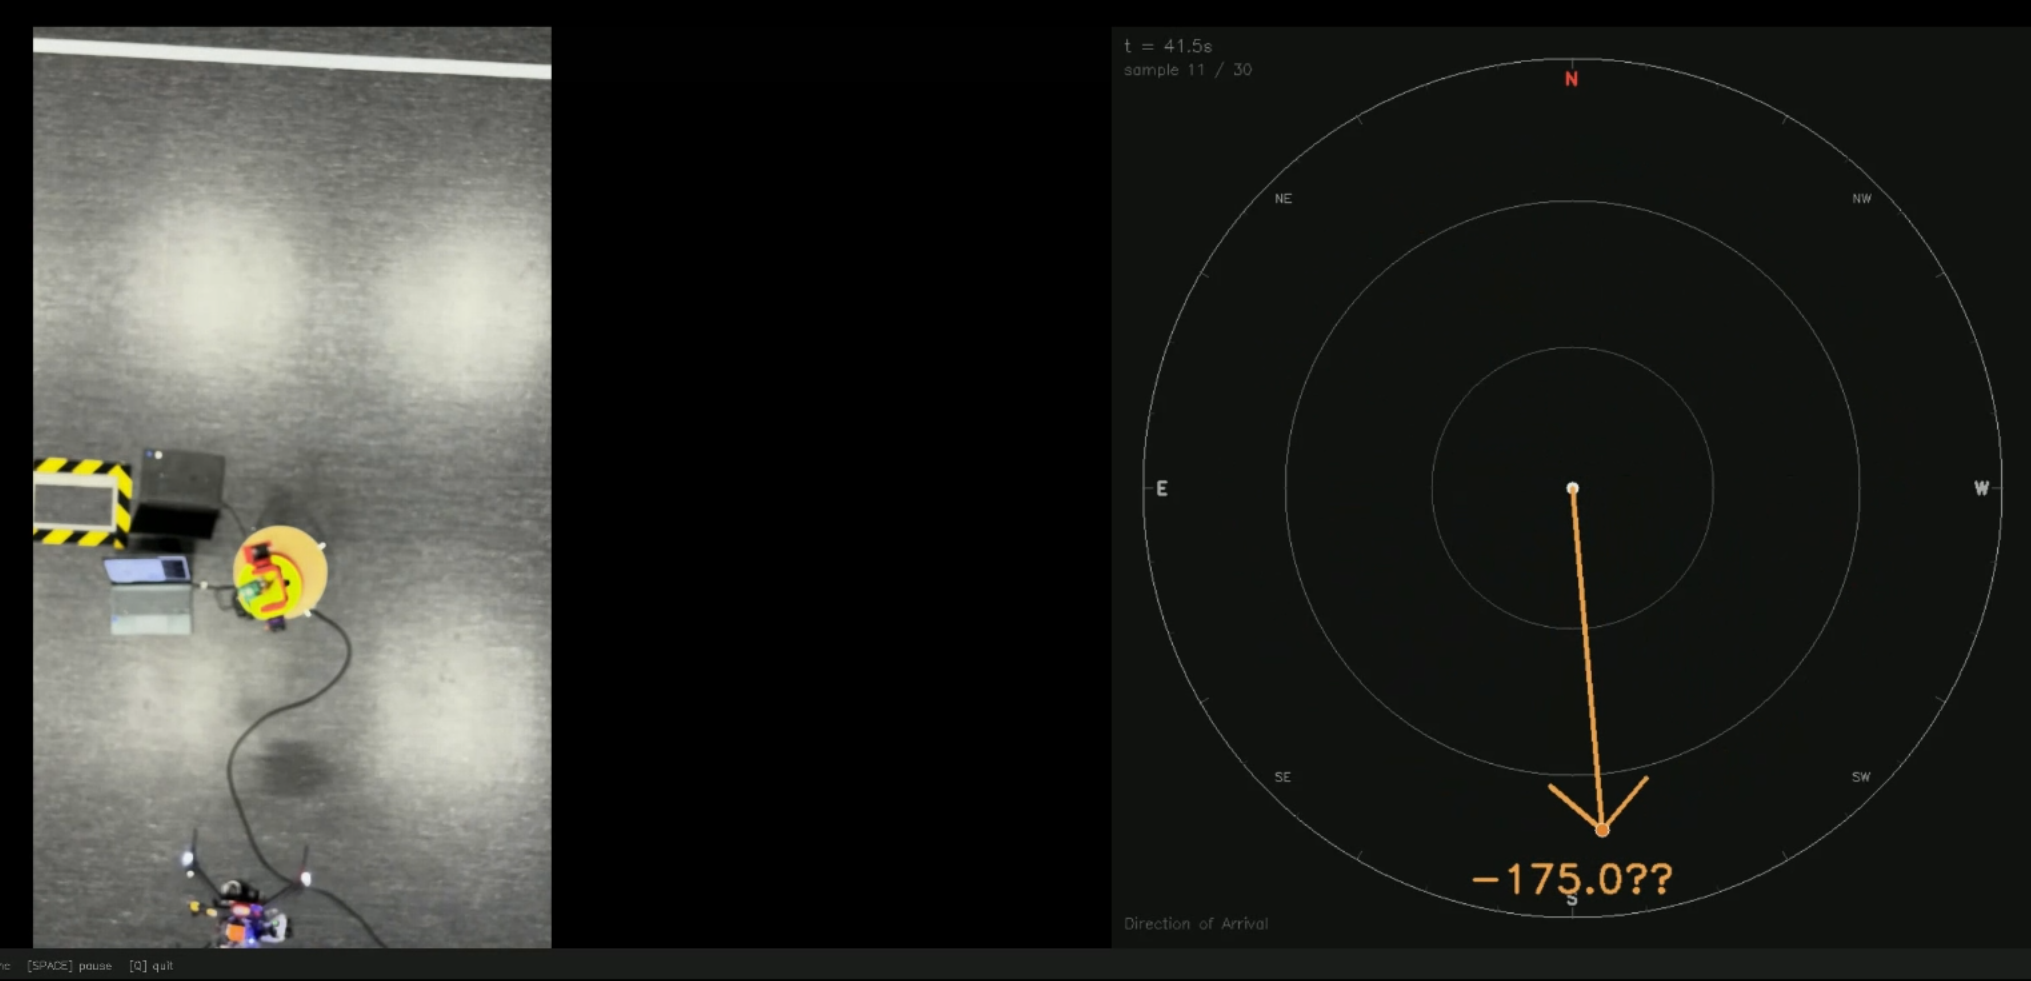
\includegraphics[width=\linewidth]{Figures/Andreas/DOA_estimation/Drone_DOA_2.png}
        \caption{}
        \label{fig:doa2}
    \end{subfigure}

    \vspace{0.5em}

    \begin{subfigure}[b]{0.48\linewidth}
        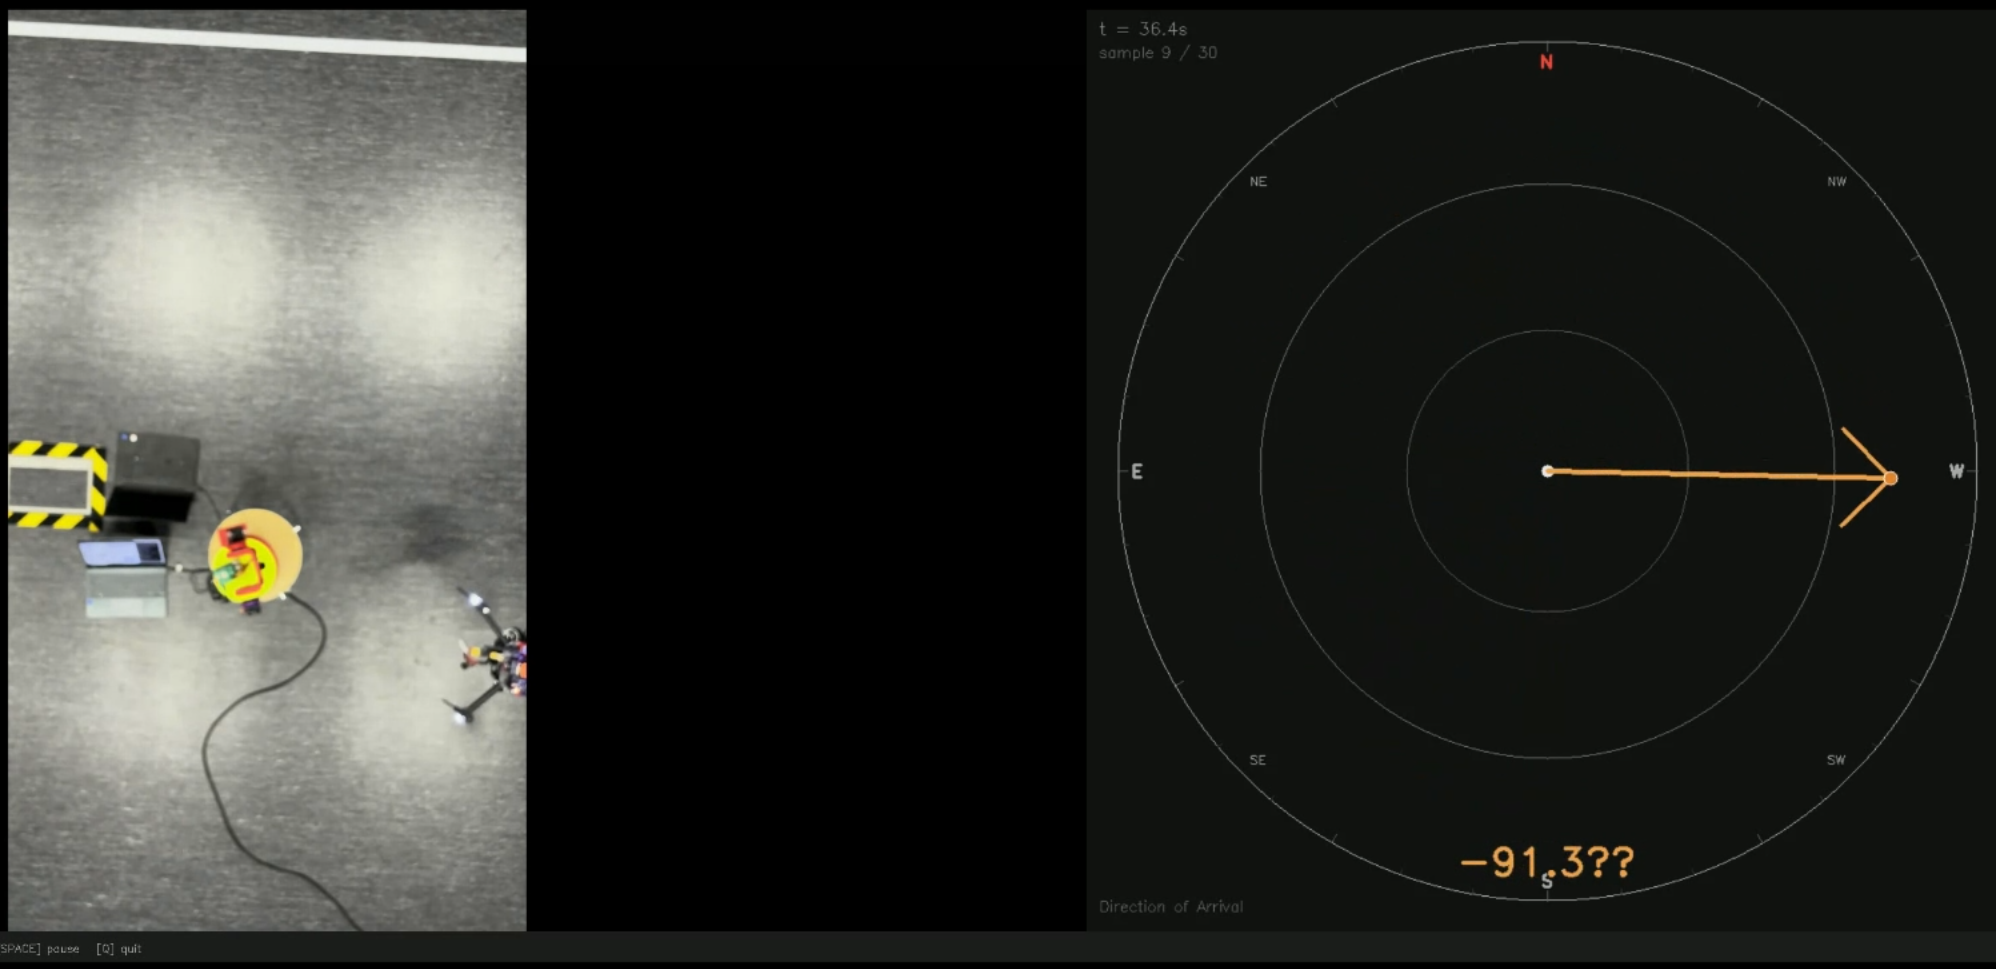
\includegraphics[width=\linewidth]{Figures/Andreas/DOA_estimation/Drone_DOA_3.png}
        \caption{}
        \label{fig:doa3}
    \end{subfigure}
    \hfill
    \begin{subfigure}[b]{0.48\linewidth}
        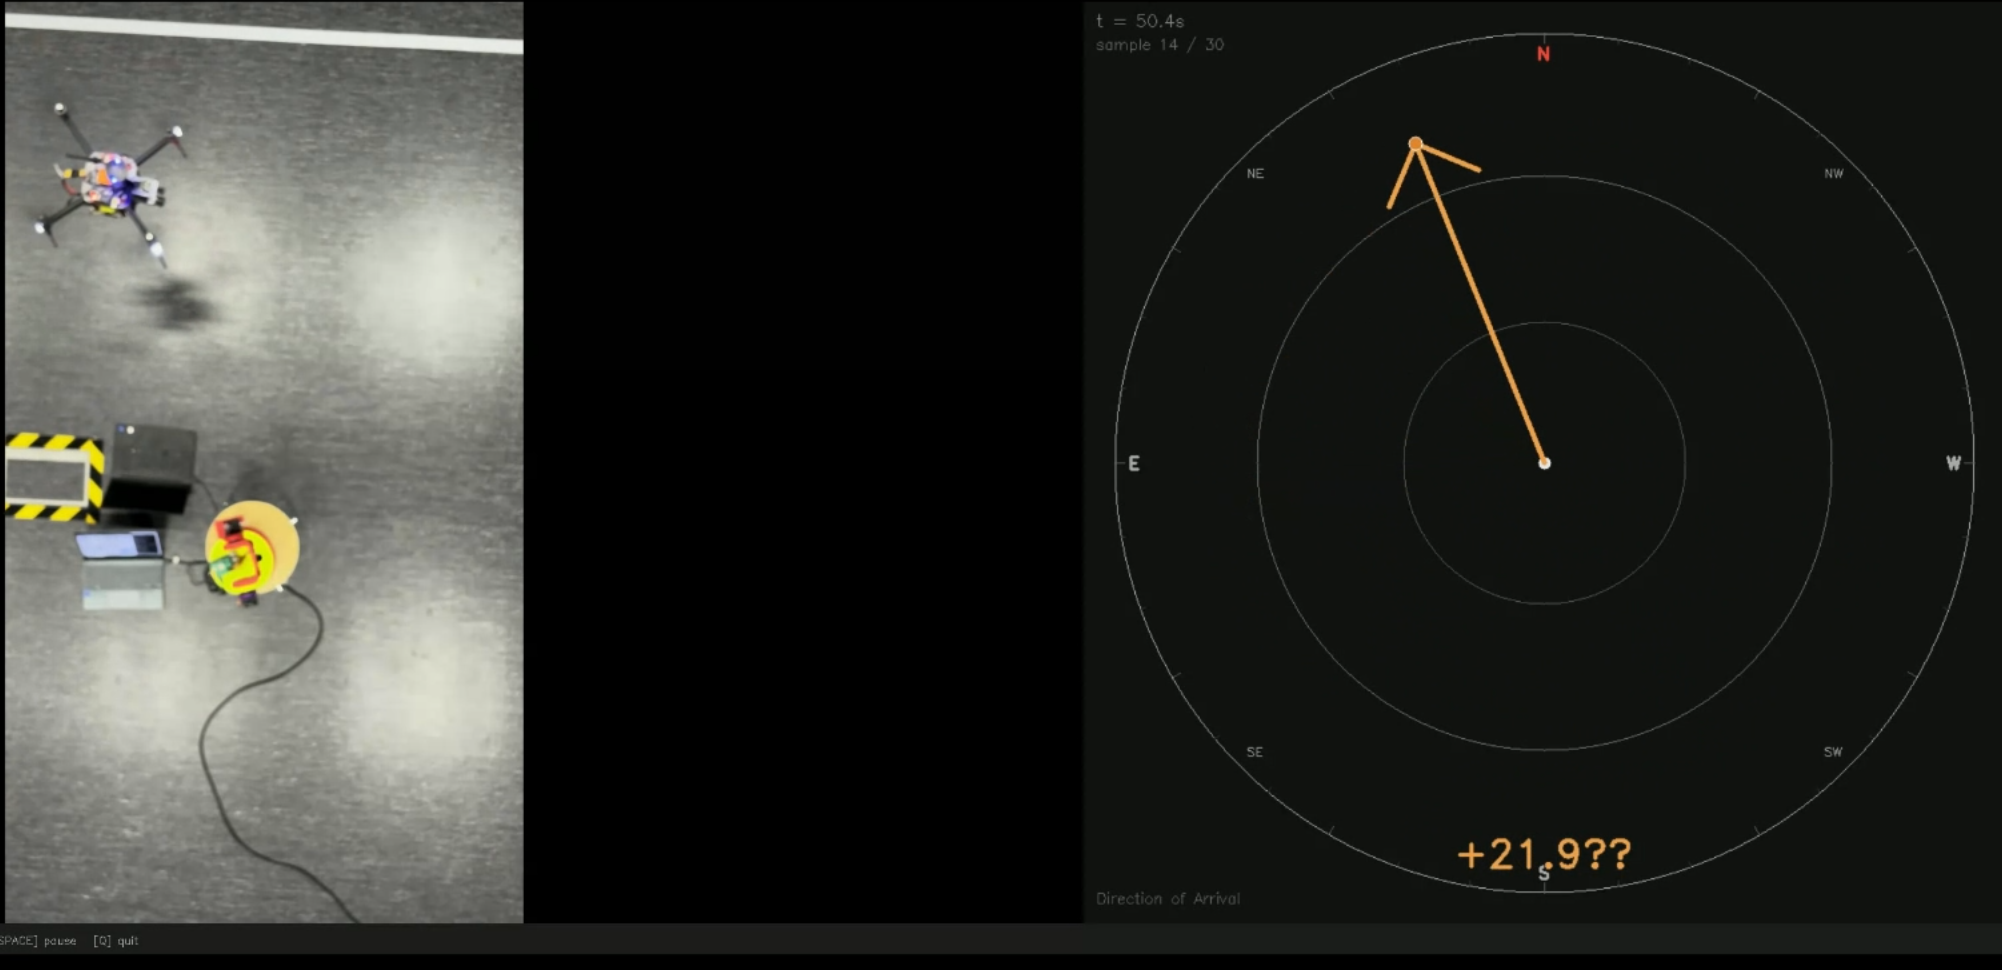
\includegraphics[width=\linewidth]{Figures/Andreas/DOA_estimation/Drone_DOA_4.png}
        \caption{}
        \label{fig:doa4}
    \end{subfigure}

    \caption{DOA estimation of the drone circulating around the tower.}
    \label{fig:doa_screenshots}
\end{figure}

The results of the Ml classification and the DOA estimation were consistent and accurate. However, it turned out during the testing process, that the lag produced by the system was more significant then expected as seen in Figure~\ref{fig:time_between_each_iteration}. The second DOA estimate was produced after around 9 seconds after the first estimation, which might be caused by the system startup. The other consecutive estimations were generated in 3.24 seconds on average. The main reason for doubling of the expected time needed for DOA estimation, might be the generation of the DOA visualization and Mel-spectrogram figures used for debuging.    

\begin{figure}[h]
    \centering
    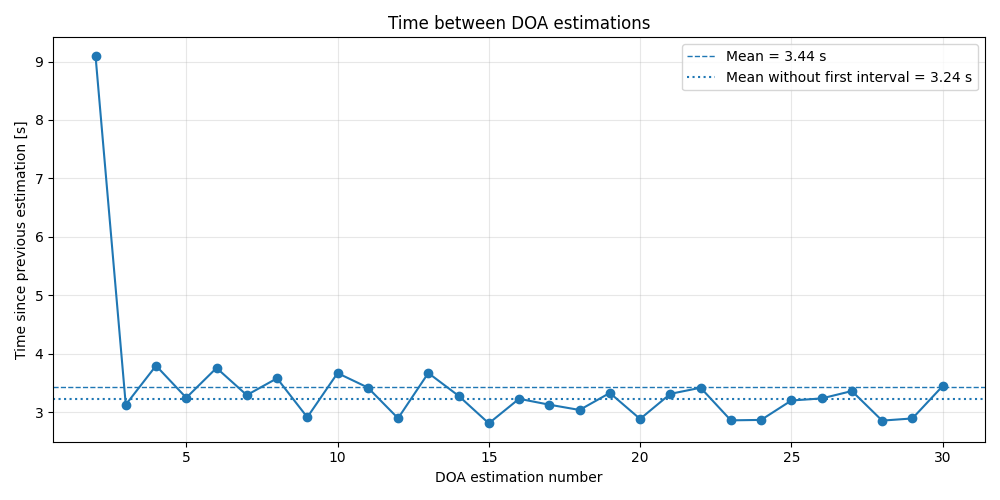
\includegraphics[width=0.5\linewidth]{Figures/time_between_each_estimation.png}
    \caption{Time between each iteration produced during the final test}
    \label{fig:time_between_each_iteration}
\end{figure}

The system lag, was later tested without the figure generation modules, which resulted in Figure~\ref{fig:time_lag_no_figure}, which shows that the lag time was indeed caused by the figure generation. The test was also conducted without the ML, which is expected to produce approx.25 ms of lag per iteration and around 250 ms during the initialization period, as seen in Figure~\ref{fig:ml_time}.

\begin{figure}[h]
    \centering
    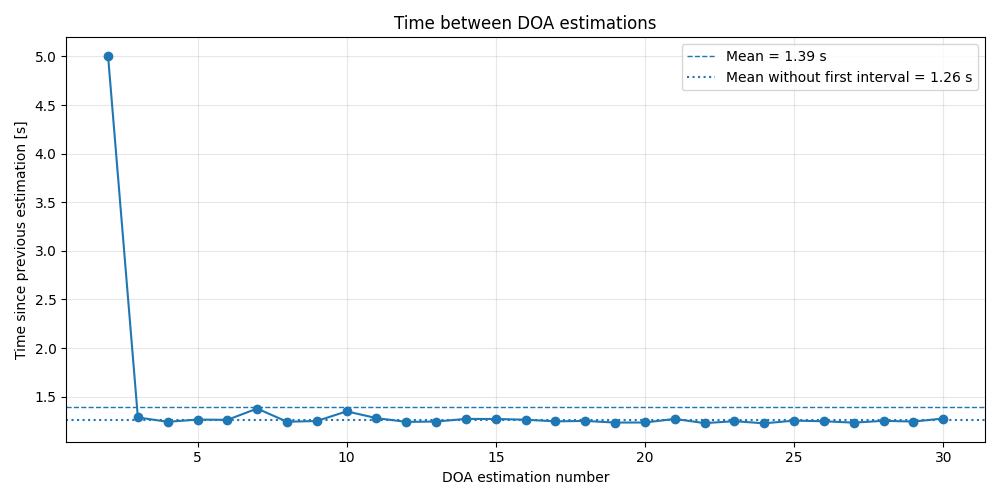
\includegraphics[width=0.5\linewidth]{Figures/time_test_without_figure_production_no_ML.png}
    \caption{Time between each iteration produced without the figure generation methods}
    \label{fig:time_lag_no_figure}
\end{figure}

\begin{figure}[h]
    \centering
    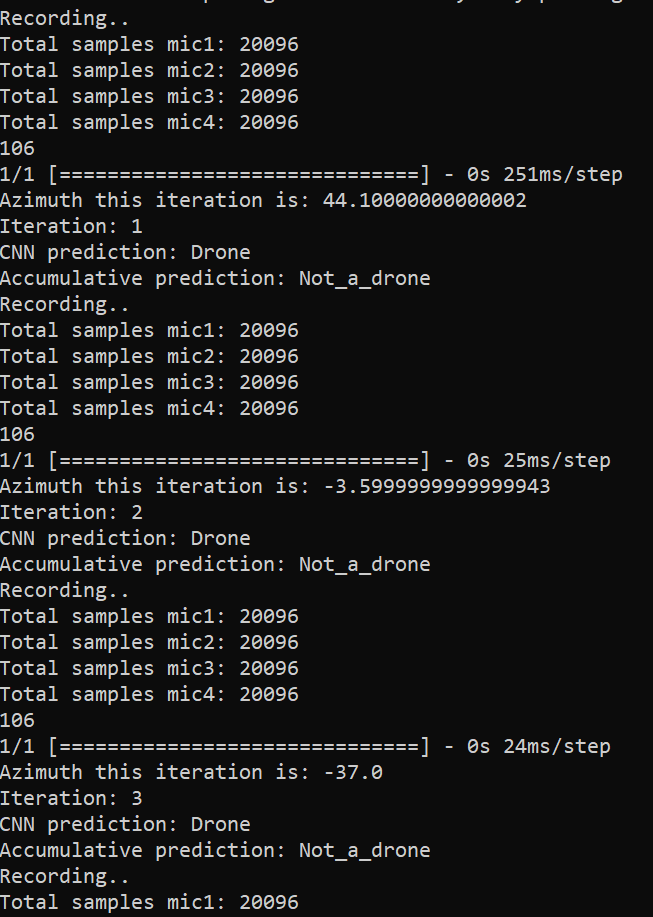
\includegraphics[width=0.3\linewidth]{Figures/times ml.png}
    \caption{Time duration needed for ML classification}
    \label{fig:ml_time}
\end{figure}

So by adding the time needed for ML to classify the sound source, the total time needed for one iteration is around 1.285 s.  

\newpage

\section{MFCC extraction}

    \subsection{Spectrogram and Mel-spectrogram representation}
    In the early stages of the signal acquisition testing, both the spectrograms and the Mel-spectrograms were generated to visualize the frequency bands present in the acquired signal. As seen in Figure~\ref{fig:spectrograms}, the Mel-spectrogram is able to represent the available frequency bands with more detail then the "normal" spectrogram. 
    
    \begin{figure}[H]
    \centering
    \begin{subfigure}[b]{0.48\textwidth}
        \centering
        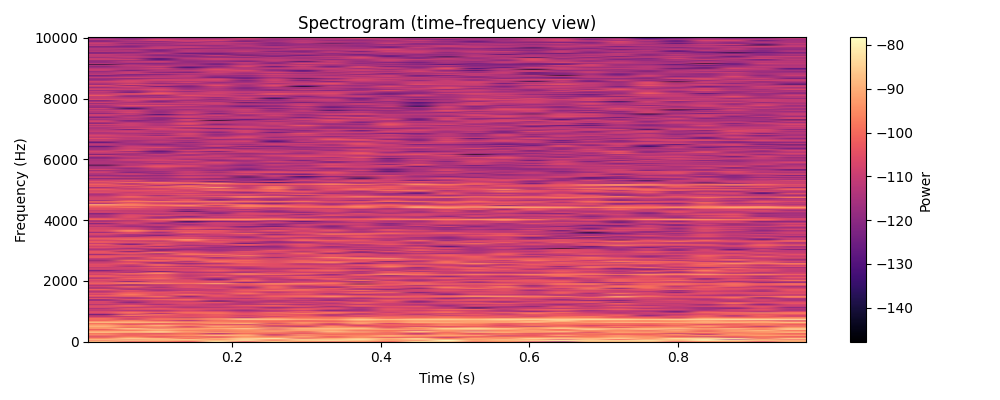
\includegraphics[width=\textwidth]{Figures/Debug_spectrogram1777884217.5826006.png}
        \caption{Spectrogram}
        \label{fig:spectrogram}
    \end{subfigure}
    \hfill
    \begin{subfigure}[b]{0.48\textwidth}
        \centering
        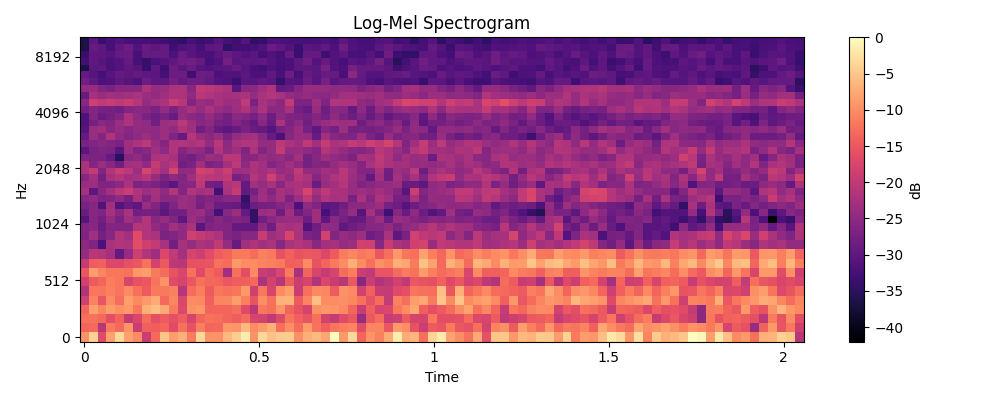
\includegraphics[width=\textwidth]{Figures/Debug_mel_spectrogram1777884217.5826006.png}
        \caption{Mel-spectrogram}
        \label{fig:mel_spectrogram}
    \end{subfigure}
    \caption{Spectrogram types generated during the testing process}
\label{fig:spectrograms}
\end{figure}

   \subsection{Mel-spectrograms from DOA testing}
    During the testing process, the system has produced different Mel-spectrograms, where each was representing unique frequency bands present in the signal. 
    
        \subsubsection{First stage: human-generated sounds}

        The behaviour of the signal representing the calpping sound can be seen in Figure~\ref{fig:clapping_mel_spec}. During the recording period, the student clapped three times, which produced three short high-energy regions in the Mel-spectrogram. The clapping sound excited a broad range of recorded frequency bands, while the strongest visible energy appears to be concentrated around approximately 3000 Hz. 

        \begin{figure}[h]
            \centering
            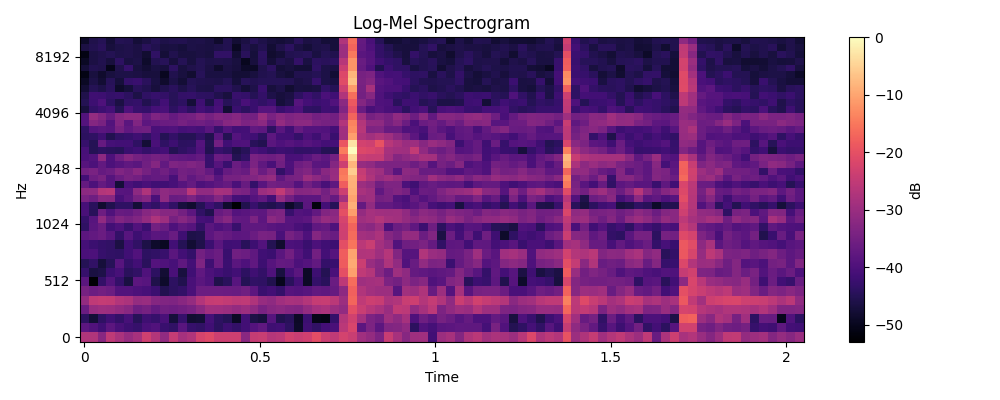
\includegraphics[width=0.75\linewidth]{Figures/Debug_mel_spectrogram1777802028.6846912.png}
            \caption{Mel-spectrogram representing the clapping sound produced during the first testing stage.}
            \label{fig:clapping_mel_spec}
        \end{figure}
\newpage
        \subsubsection{Second stage: drone-like and recorded drone sounds}

        The behaviour of the DC-motor signal. which was meant to imitate the drone sound can be seen in Figure~\ref{fig:mel_spec_dc_motor}. The signal produced several short high-energy regions, mostly concentrated around the lower frequency bands. The DC-sound compared to the clapping sound, seamed to be less consistent over time, and wasn't at all hearable by the system at the distance greater then 30 cm.

        \begin{figure}[h]
            \centering
            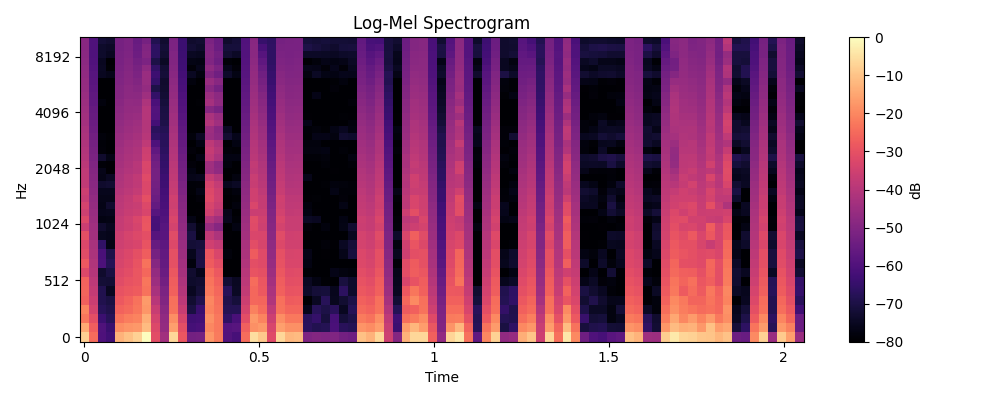
\includegraphics[width=0.75\linewidth]{Figures/Debug_mel_spectrogram1777725034.3948312.png}
            \caption{Mel-spectrogram representing the sound produced by the DC-motor}
            \label{fig:mel_spec_dc_motor}
        \end{figure}
\newpage
        The drone sound produced by the youtube video can be seen in Figure~\ref{fig:mel_spec_youtube}. Compared with the DC-motor signal, the recorded drone sound produced more continuous and stable frequency components over time. Several horizontal bands are visible in the Mel-spectrogram, especially in the lower and middle frequency range. This indicates, that the drone recording contained some harmonic components, which allowed for accurate and consistent DOA estimation of the sound source, when the phone volume was set to maximum. 

        \begin{figure}[h]
            \centering
            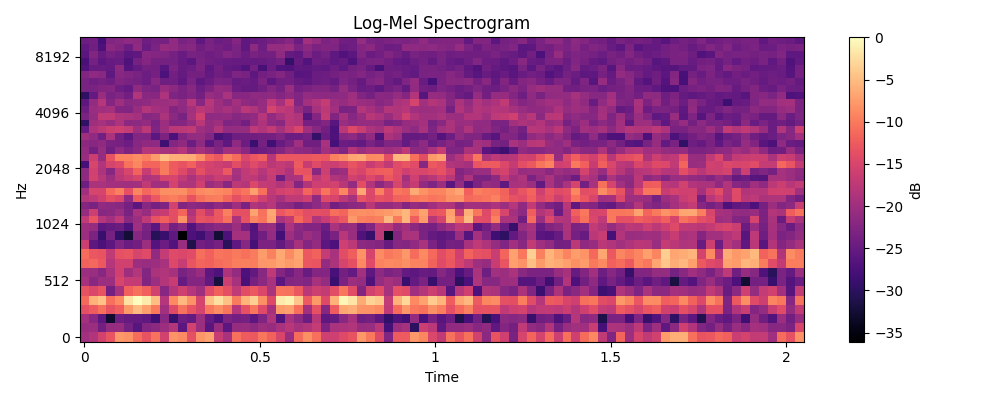
\includegraphics[width=0.75\linewidth]{Figures/Debug_mel_spectrogram1777804261.3530798.png}
            \caption{Mel-spectrogram representing the drone sound produced by the youtube video}
            \label{fig:mel_spec_youtube}
        \end{figure}
        
        \subsubsection{Third stage: live drone sound}

        The sound produced by the live drone showed similar horizontal bands to the drone sound played from the video, especially in the lower frequency range. However, the live-drone spectrogram appeared to contain less high-frequency content, as seen in Figure~\ref{fig:mel_spec_live_drone}. This difference may be related to the different test conditions. The live-drone test was conducted in the laboratory, where room reflections, background noise, and the shorter distance between the drone and the tower may have affected the recorded frequency content. In addition, the live drone produced a significantly louder acoustic signal than the phone playback, which likely made the lower-frequency drone components more dominant in the recording.

        \begin{figure}[h]
            \centering
            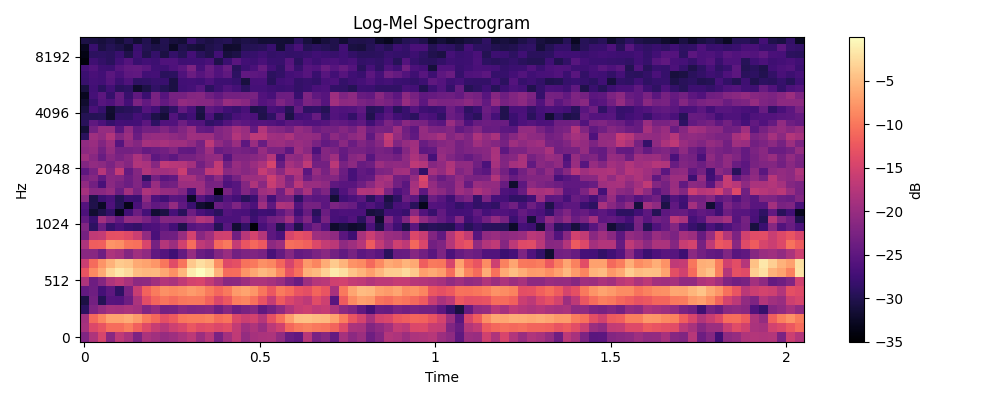
\includegraphics[width=0.75\linewidth]{Figures/Debug_mel_spectrogram1778753123.3731422.png}
            \caption{Mel-spectrogram representing the sound produced by the live-drone}
            \label{fig:mel_spec_live_drone}
        \end{figure}
        \newpage

        The Mel-spectrograms used during the system testing showed clear differnces between the tested sound sources. The clapping sound produced short boradband energy source, while the sound produced by drone, either from the youtube video, or the live-drone, produced the continous horizontal frequency bands. The visual comparison between the signals, has also shown how big of an influnece the testing enviroment can have on the noise present in the deteced signal. Therefore, the Mel-spectrograms privided useful support for system testing and training of the ML algorithm. 
          
    %mention the need of redesigning the pcb, to use another motor drive

\section{YOLO Hardware test}
The average intereference time with the HAILO chip was found to be 9.2ms whereas with CPU only it was 235.6ms. (\ref{fig:Interference_comp}) The Raspberry PI 5 was therefore found to be able to run the YOLO detection model at around 108 intereferences pr second, whereas for CPU only it was around 3.75. 

\begin{figure}[H]
    \centering
    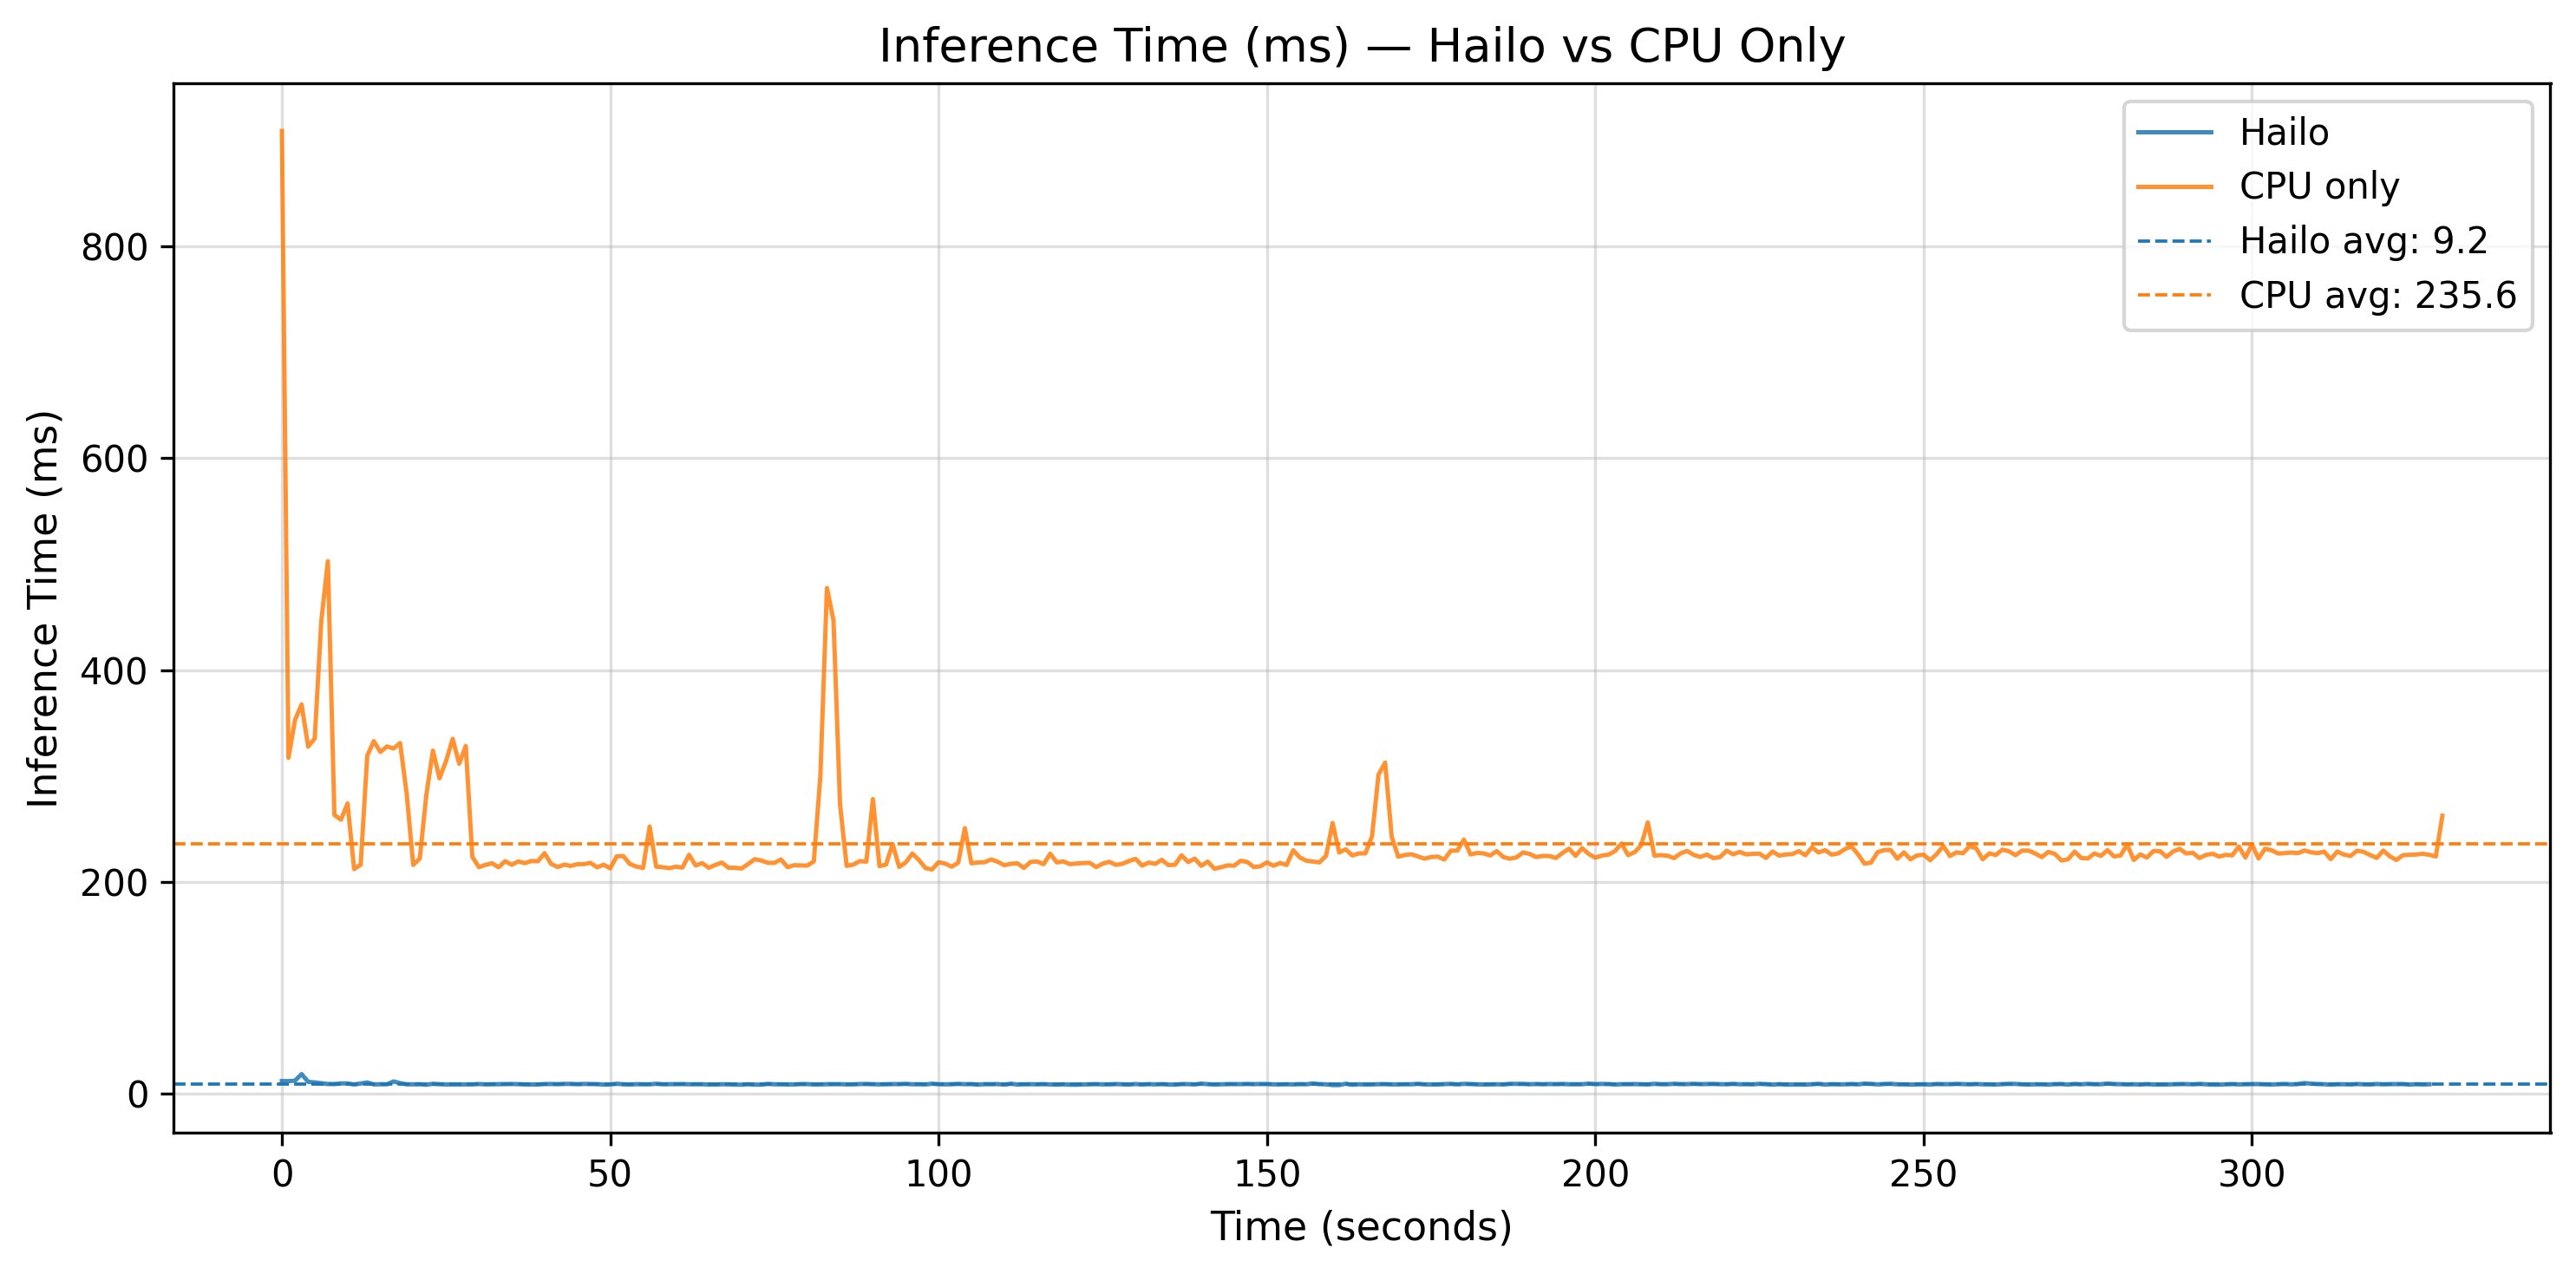
\includegraphics[width=0.95\linewidth]{Figures/Andreas/Hardware/avg_inference_ms_comparison.png}
    \caption[Interference Comparison]{Interference comparison between using the HAILO chip and CPU only, with the HAILO average interefence time being 9.2ms and with CPU only being 235.6ms.}
    \label{fig:Interference_comp}
\end{figure}

It was found that the CPU usage with the HAILO chip was at 29.7\% on average, where as without the CPU usage was found to be 92.5\% on average.(\ref{fig:cpu_usage_comparison}) Similarily the average CPU temperature with the HAILO chip was found to be 54.1 $C\degree$ where as with CPU only the average temperature rose to an average of 71 $C\degree$ (\ref{fig:cpu_temp_comparison})

\begin{figure}[H]
    \centering
    \begin{subfigure}[b]{0.48\textwidth}
        \centering
        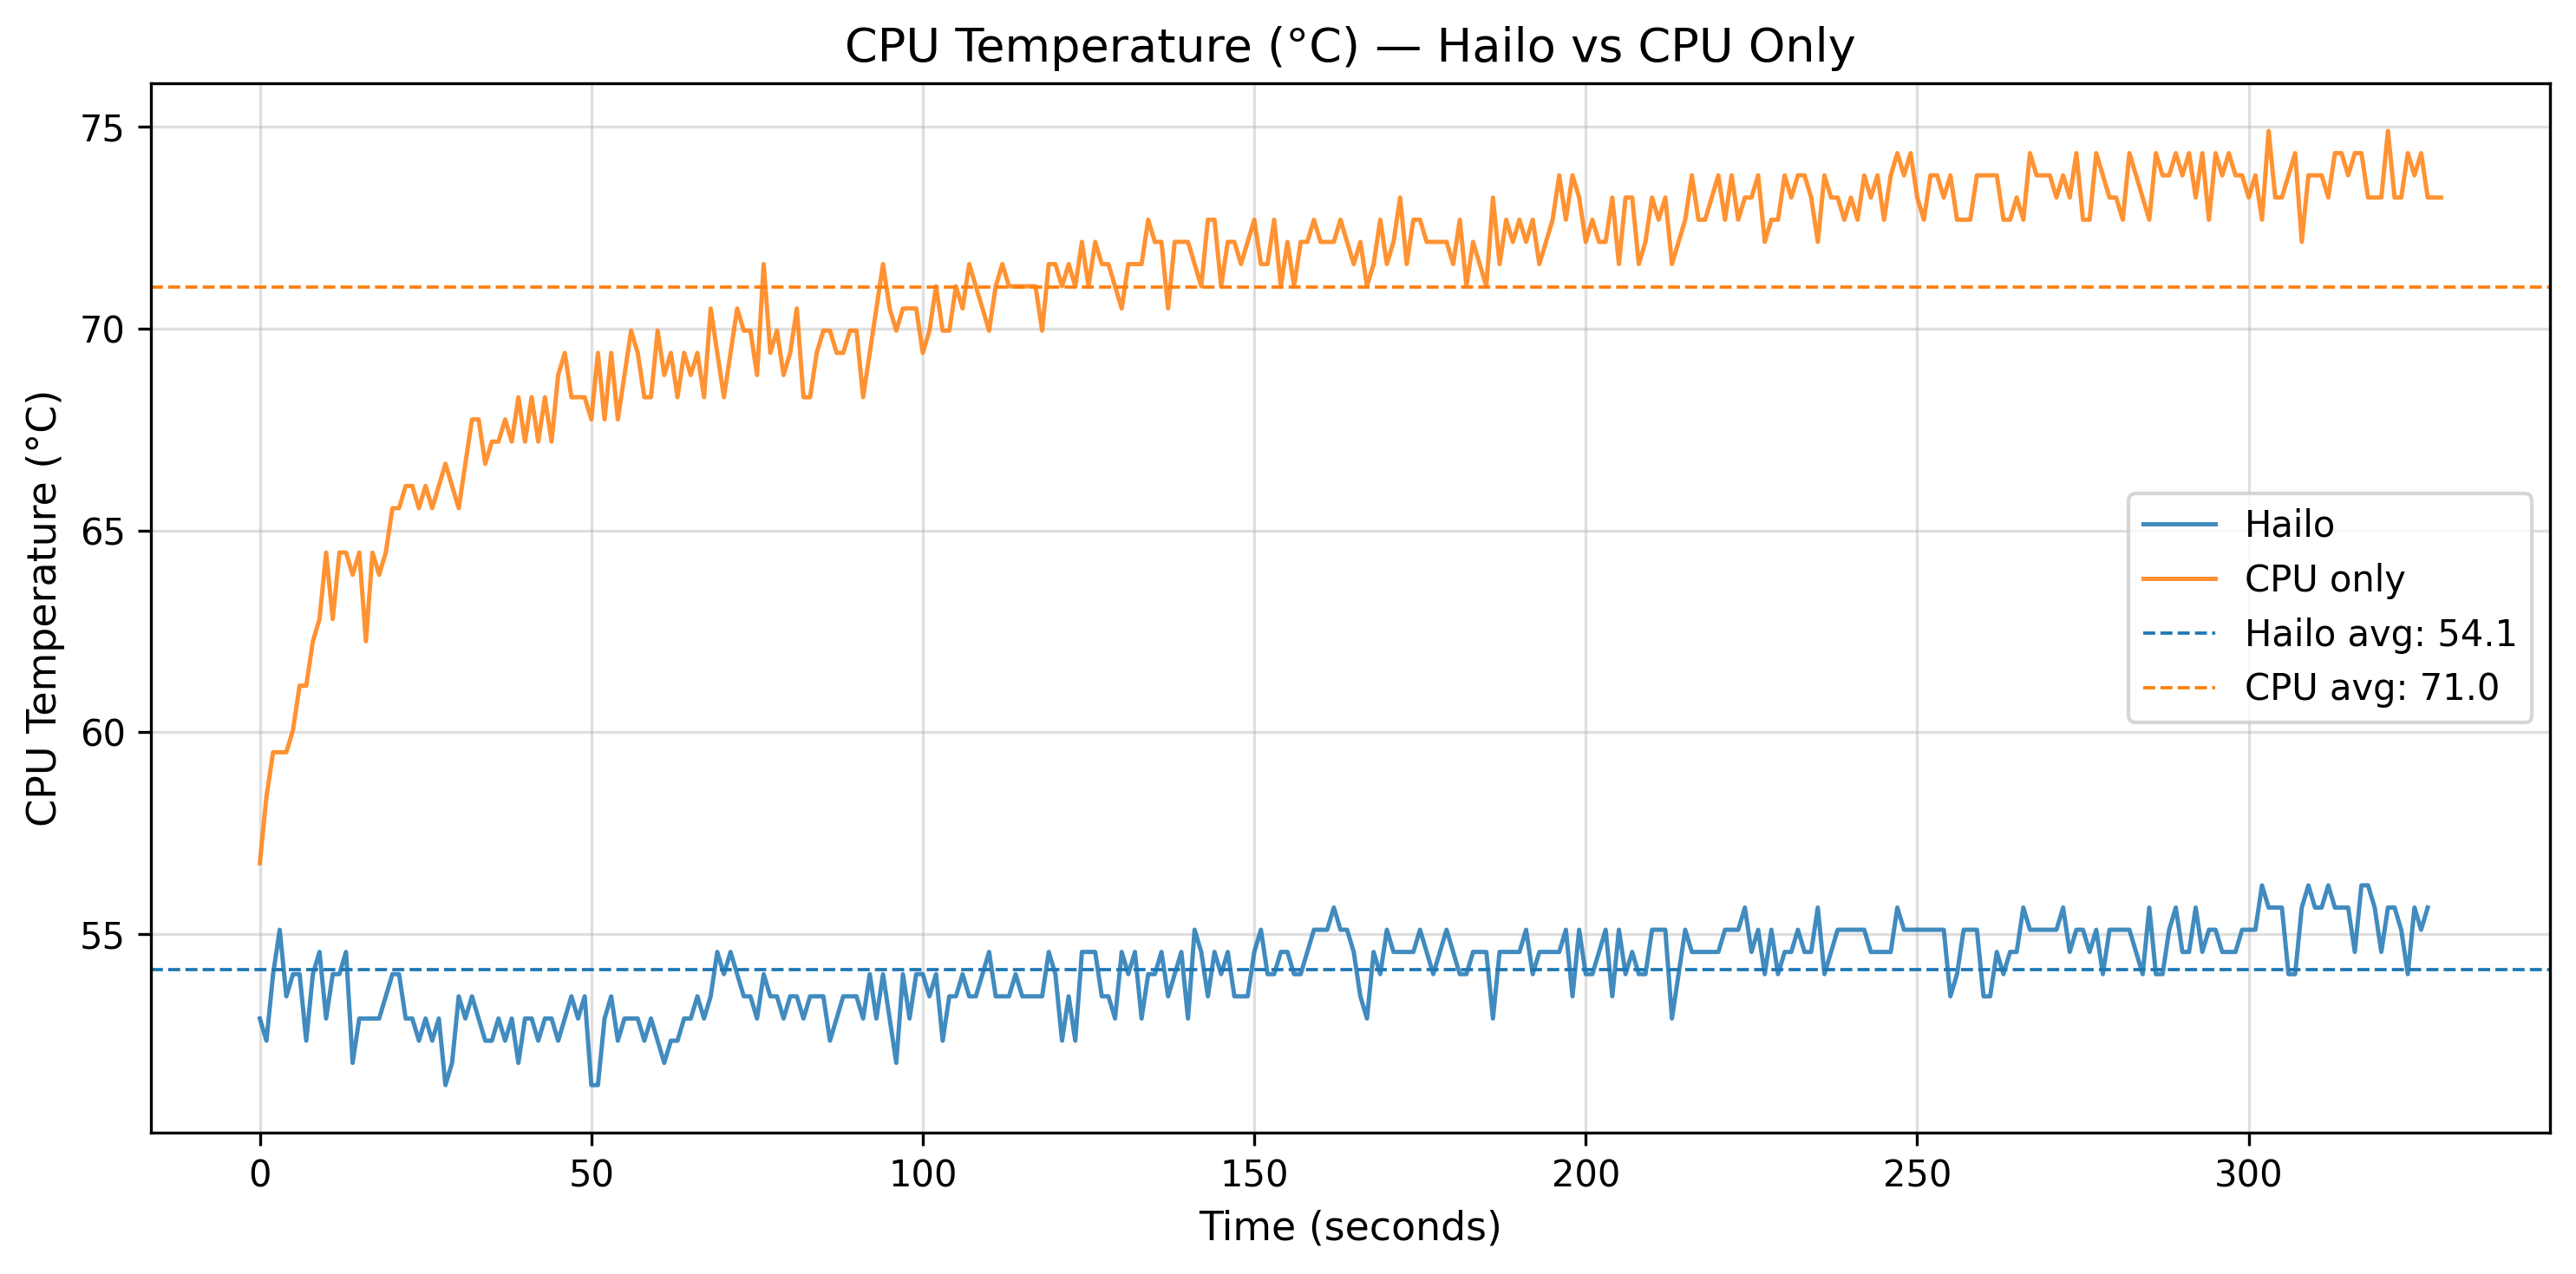
\includegraphics[width=\textwidth]{Figures/Andreas/Hardware/cpu_temp_c_comparison.png}
        \caption{CPU temperature comparison}
        \label{fig:cpu_temp_comparison}
    \end{subfigure}
    \hfill
    \begin{subfigure}[b]{0.48\textwidth}
        \centering
        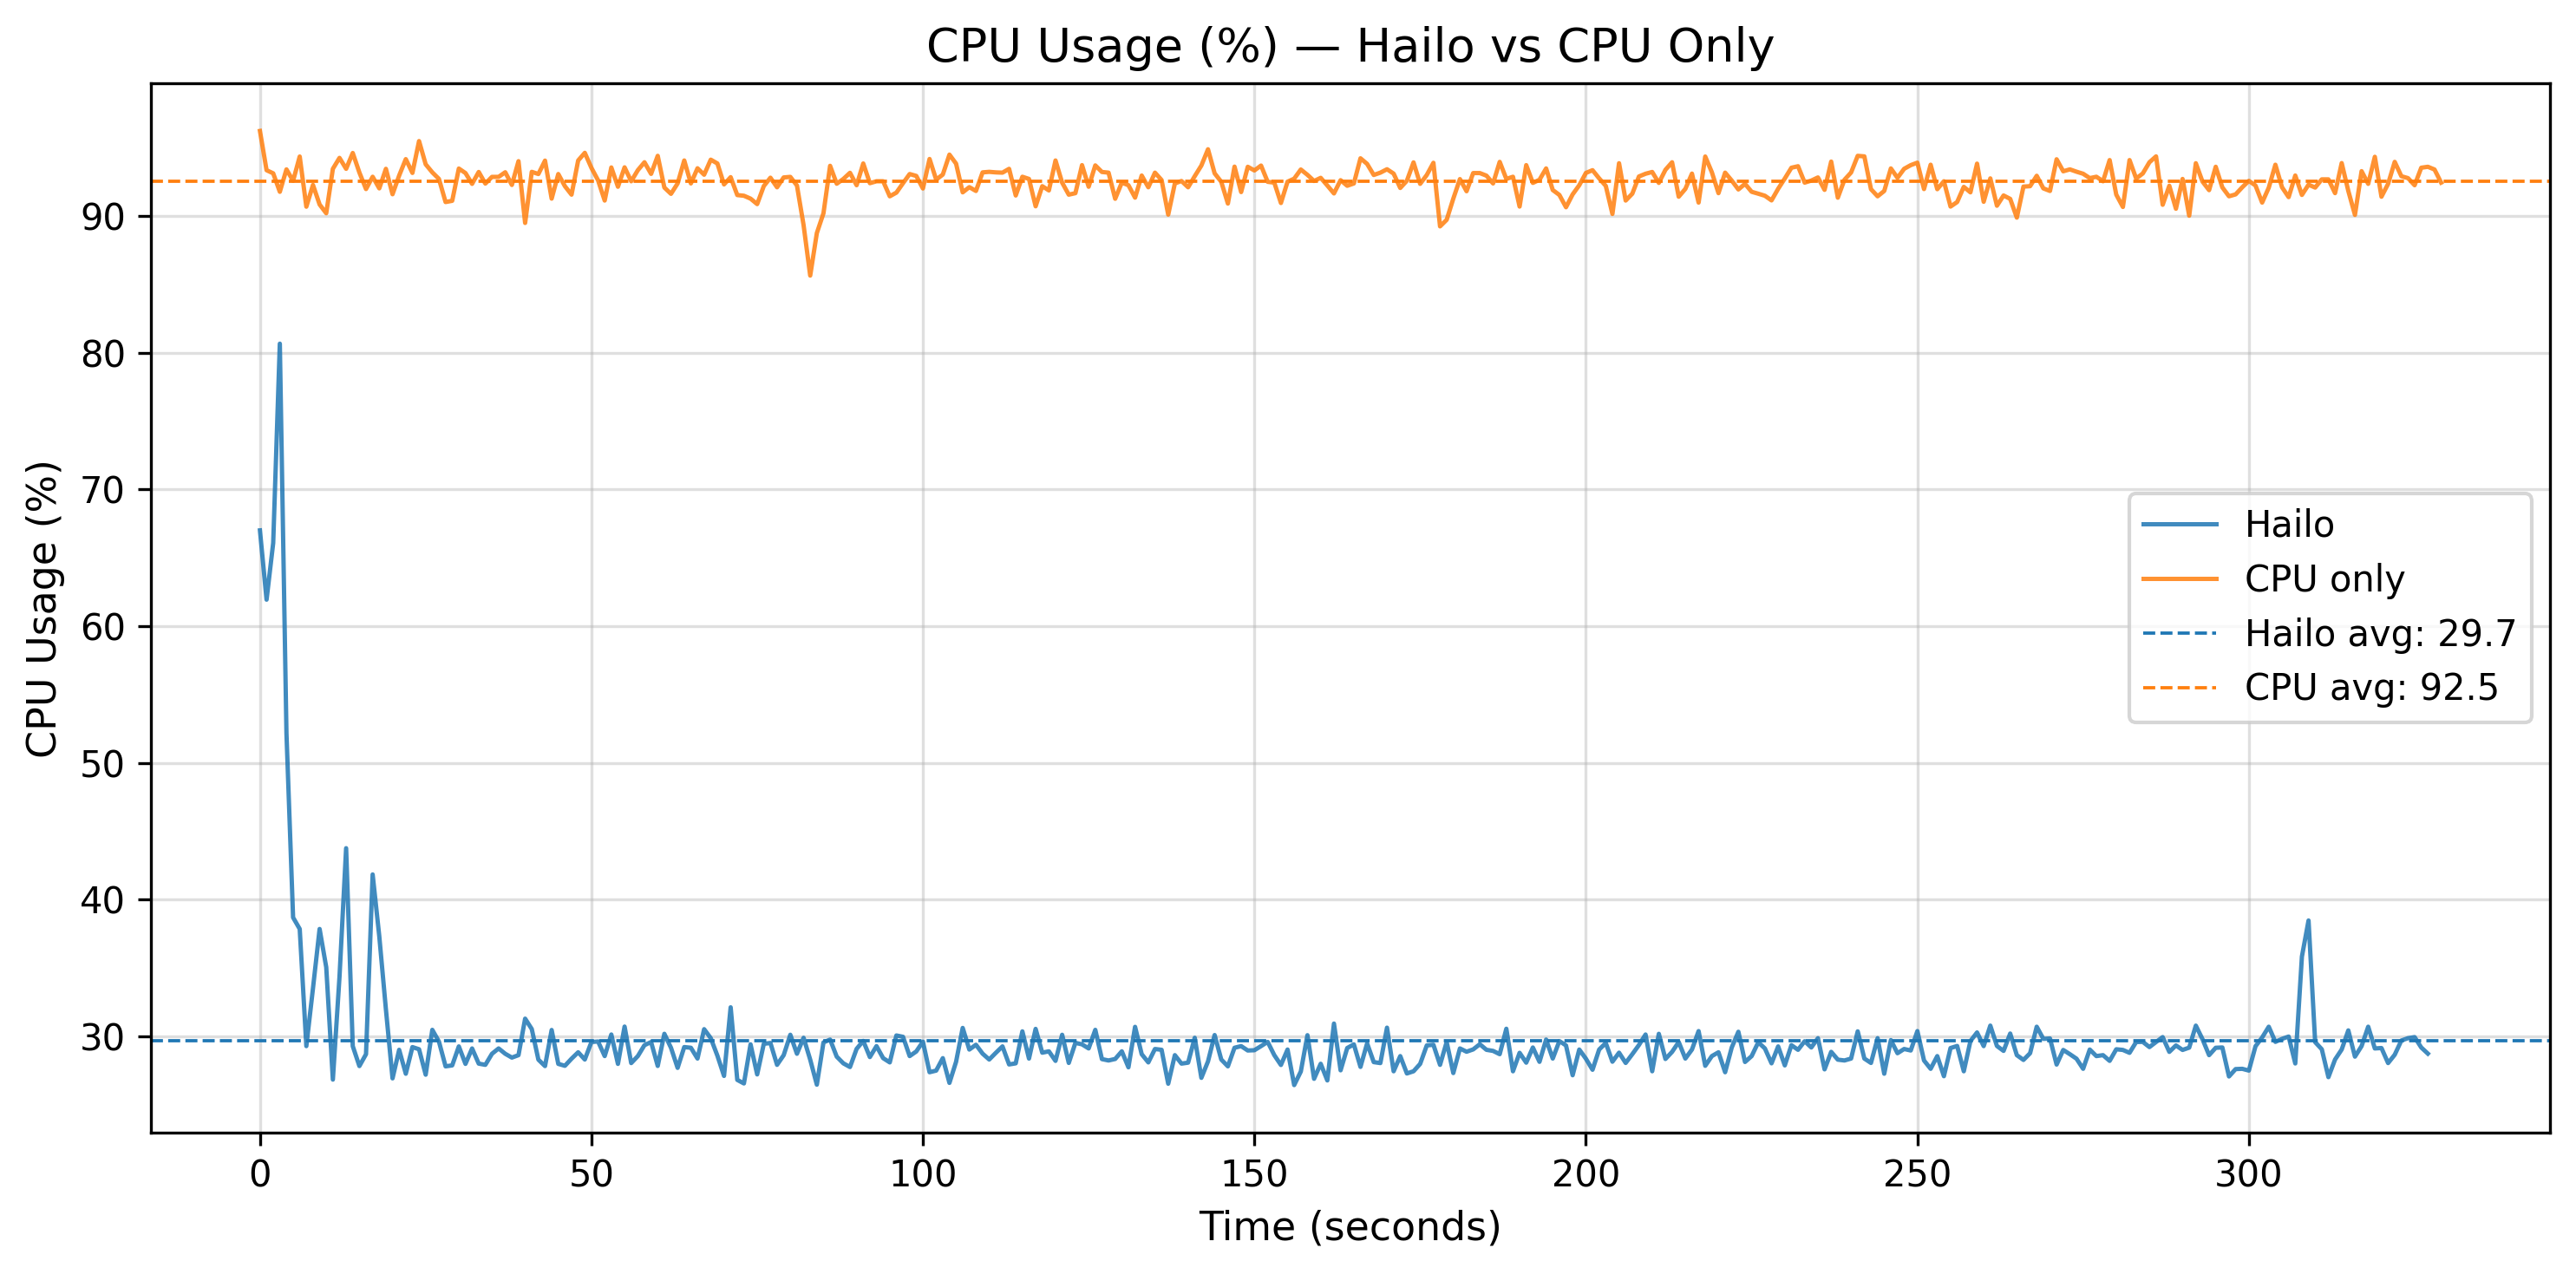
\includegraphics[width=\textwidth]{Figures/Andreas/Hardware/cpu_usage_pct_comparison.png}
        \caption{CPU usage comparison}
        \label{fig:cpu_usage_comparison}
    \end{subfigure}
    \caption{CPU temperature and usage during Hailo and CPU-only inference pipelines. The average CPU temperature and usage with the HAILO chip were 54.1 C$\degree$   and 29.7 \% respectively}
    \label{fig:cpu_comparison}
\end{figure}

The RAM usage was found to be similar both with and without the HAILO chip (\ref{fig:RAM Usage})

\begin{figure}[H]
    \centering
    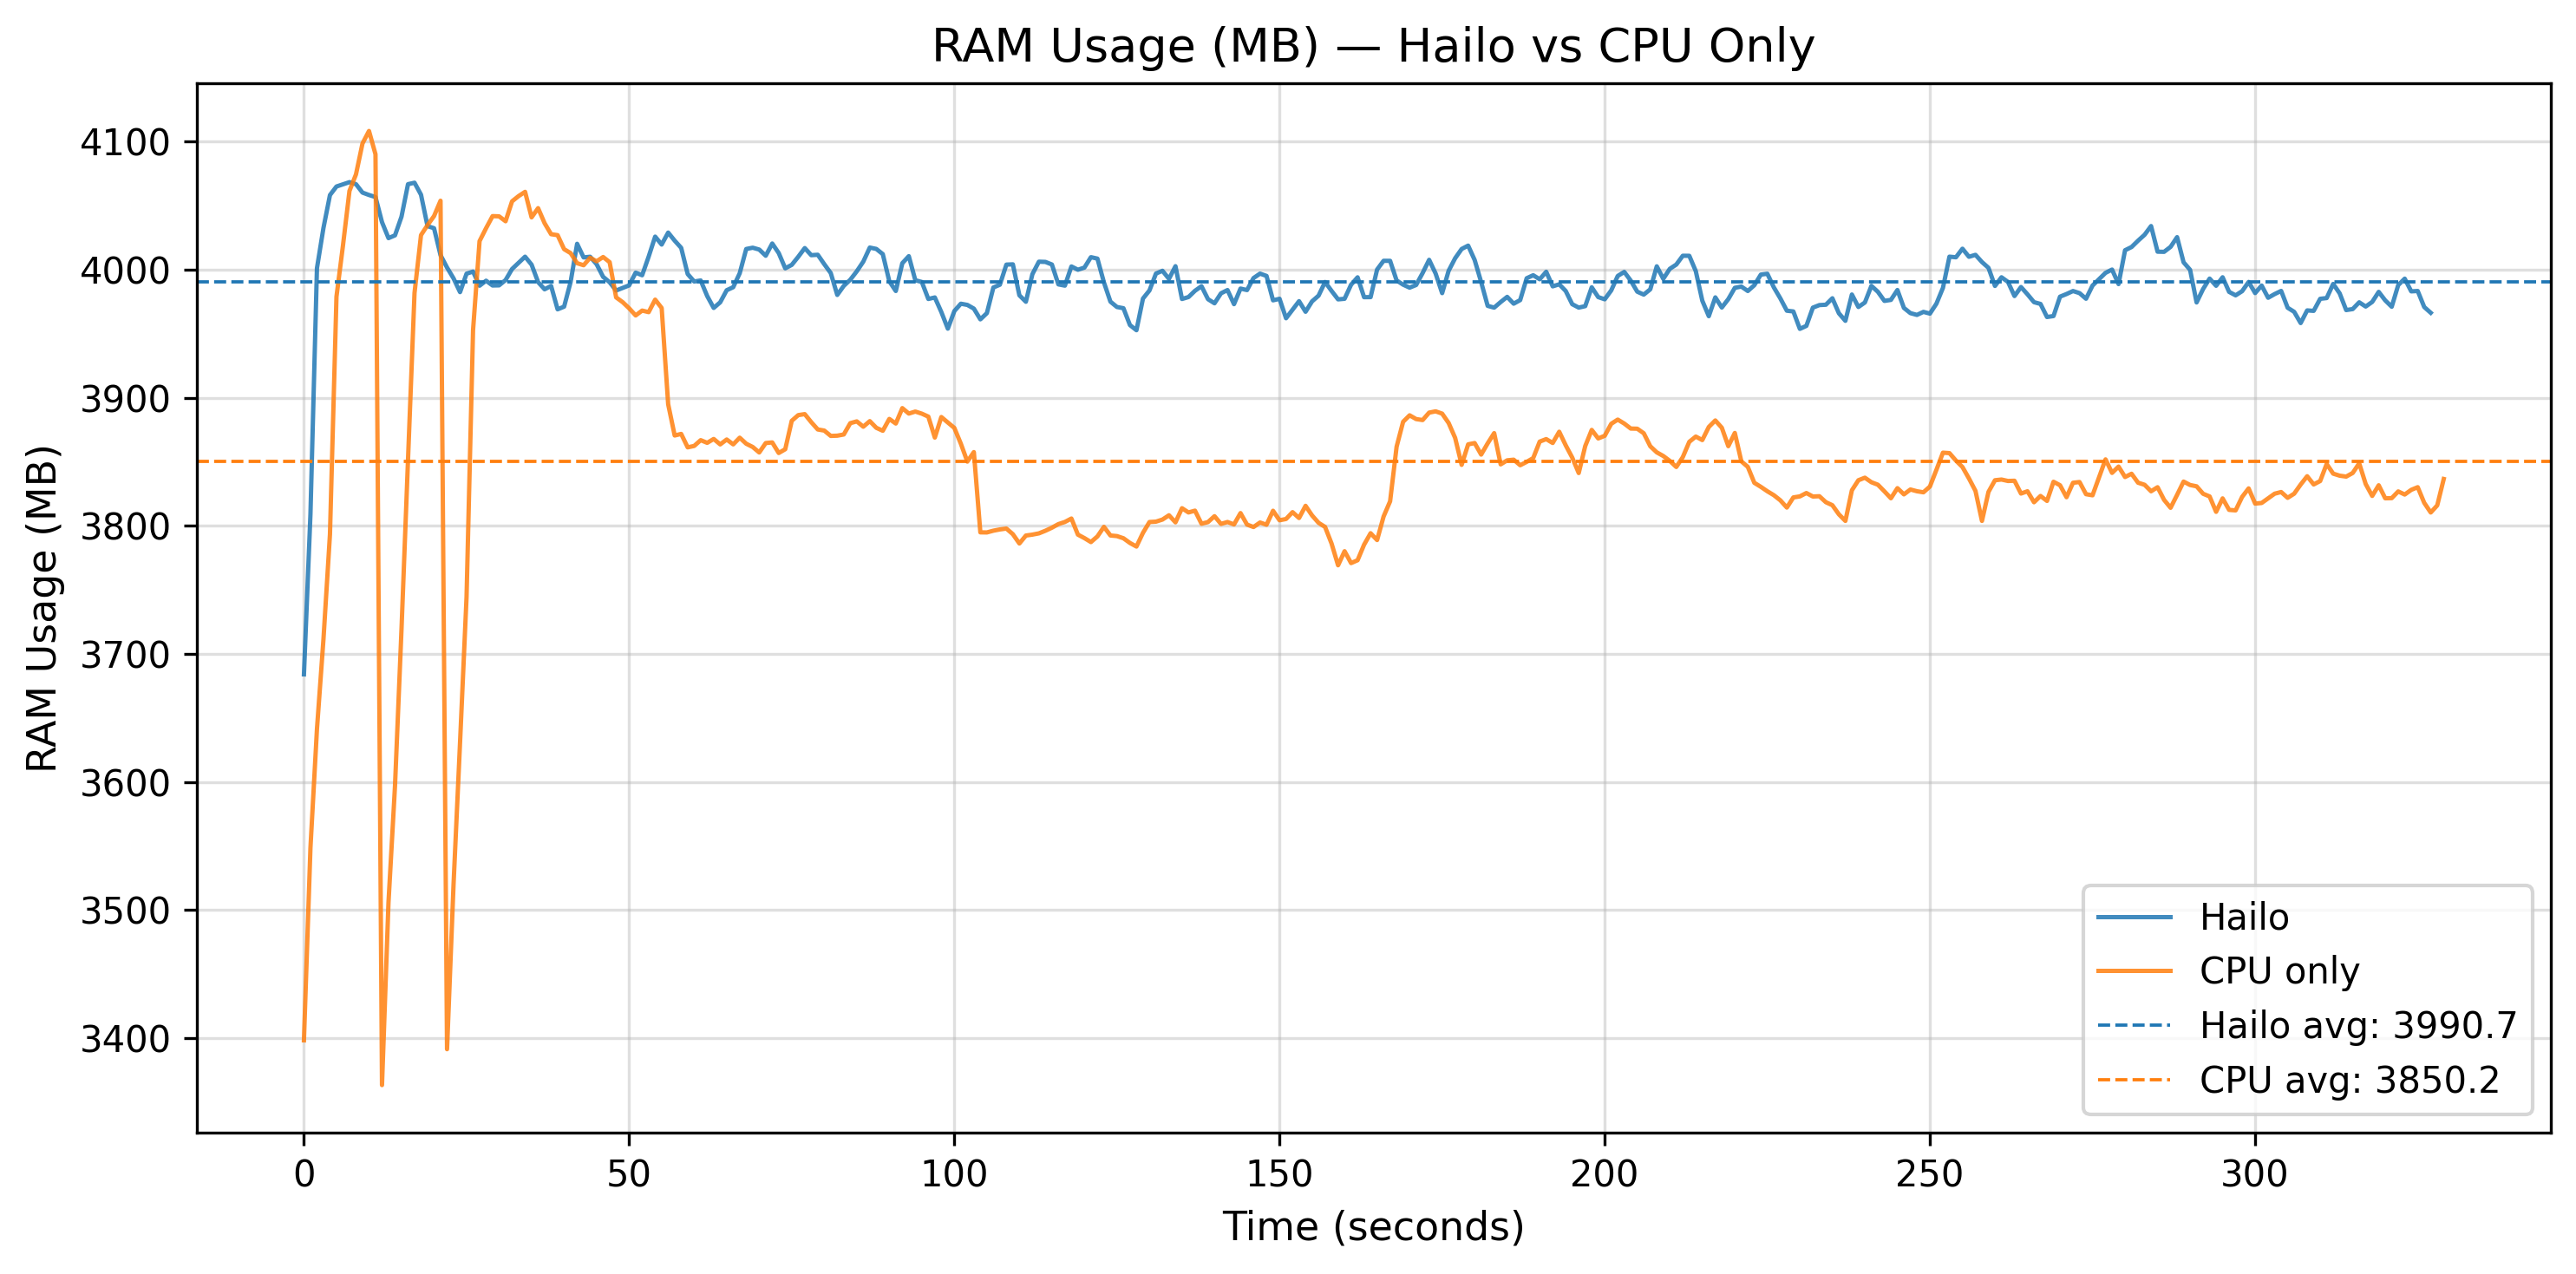
\includegraphics[width=0.95\linewidth]{Figures/Andreas/Hardware/ram_used_mb_comparison.png}
    \caption[RAM usage]{RAM usage on the RPI with and without the HAILO AI chip. }
    \label{fig:RAM Usage}
\end{figure}



\section{YOLO results}
\subsection{Training results}
The training on the final YOLO model lasted for about 11.5 hours with the model converging on 43 epochs with each epoch taking around 16 minutes to complete. The three main training losses, box, classification and DFL declined consistently throughout the training (fig: \ref{fig:pYolo_results}). The val box loss has a slight increase after epoct 25 (0.02), indicating some overfitting on the bounding box regression (fig: \ref{fig:pYolo_results}). The val classification loss has a high scale compared to the training classification loss (fig: \ref{fig:pYolo_results}).

\begin{figure}[H]
    \centering
    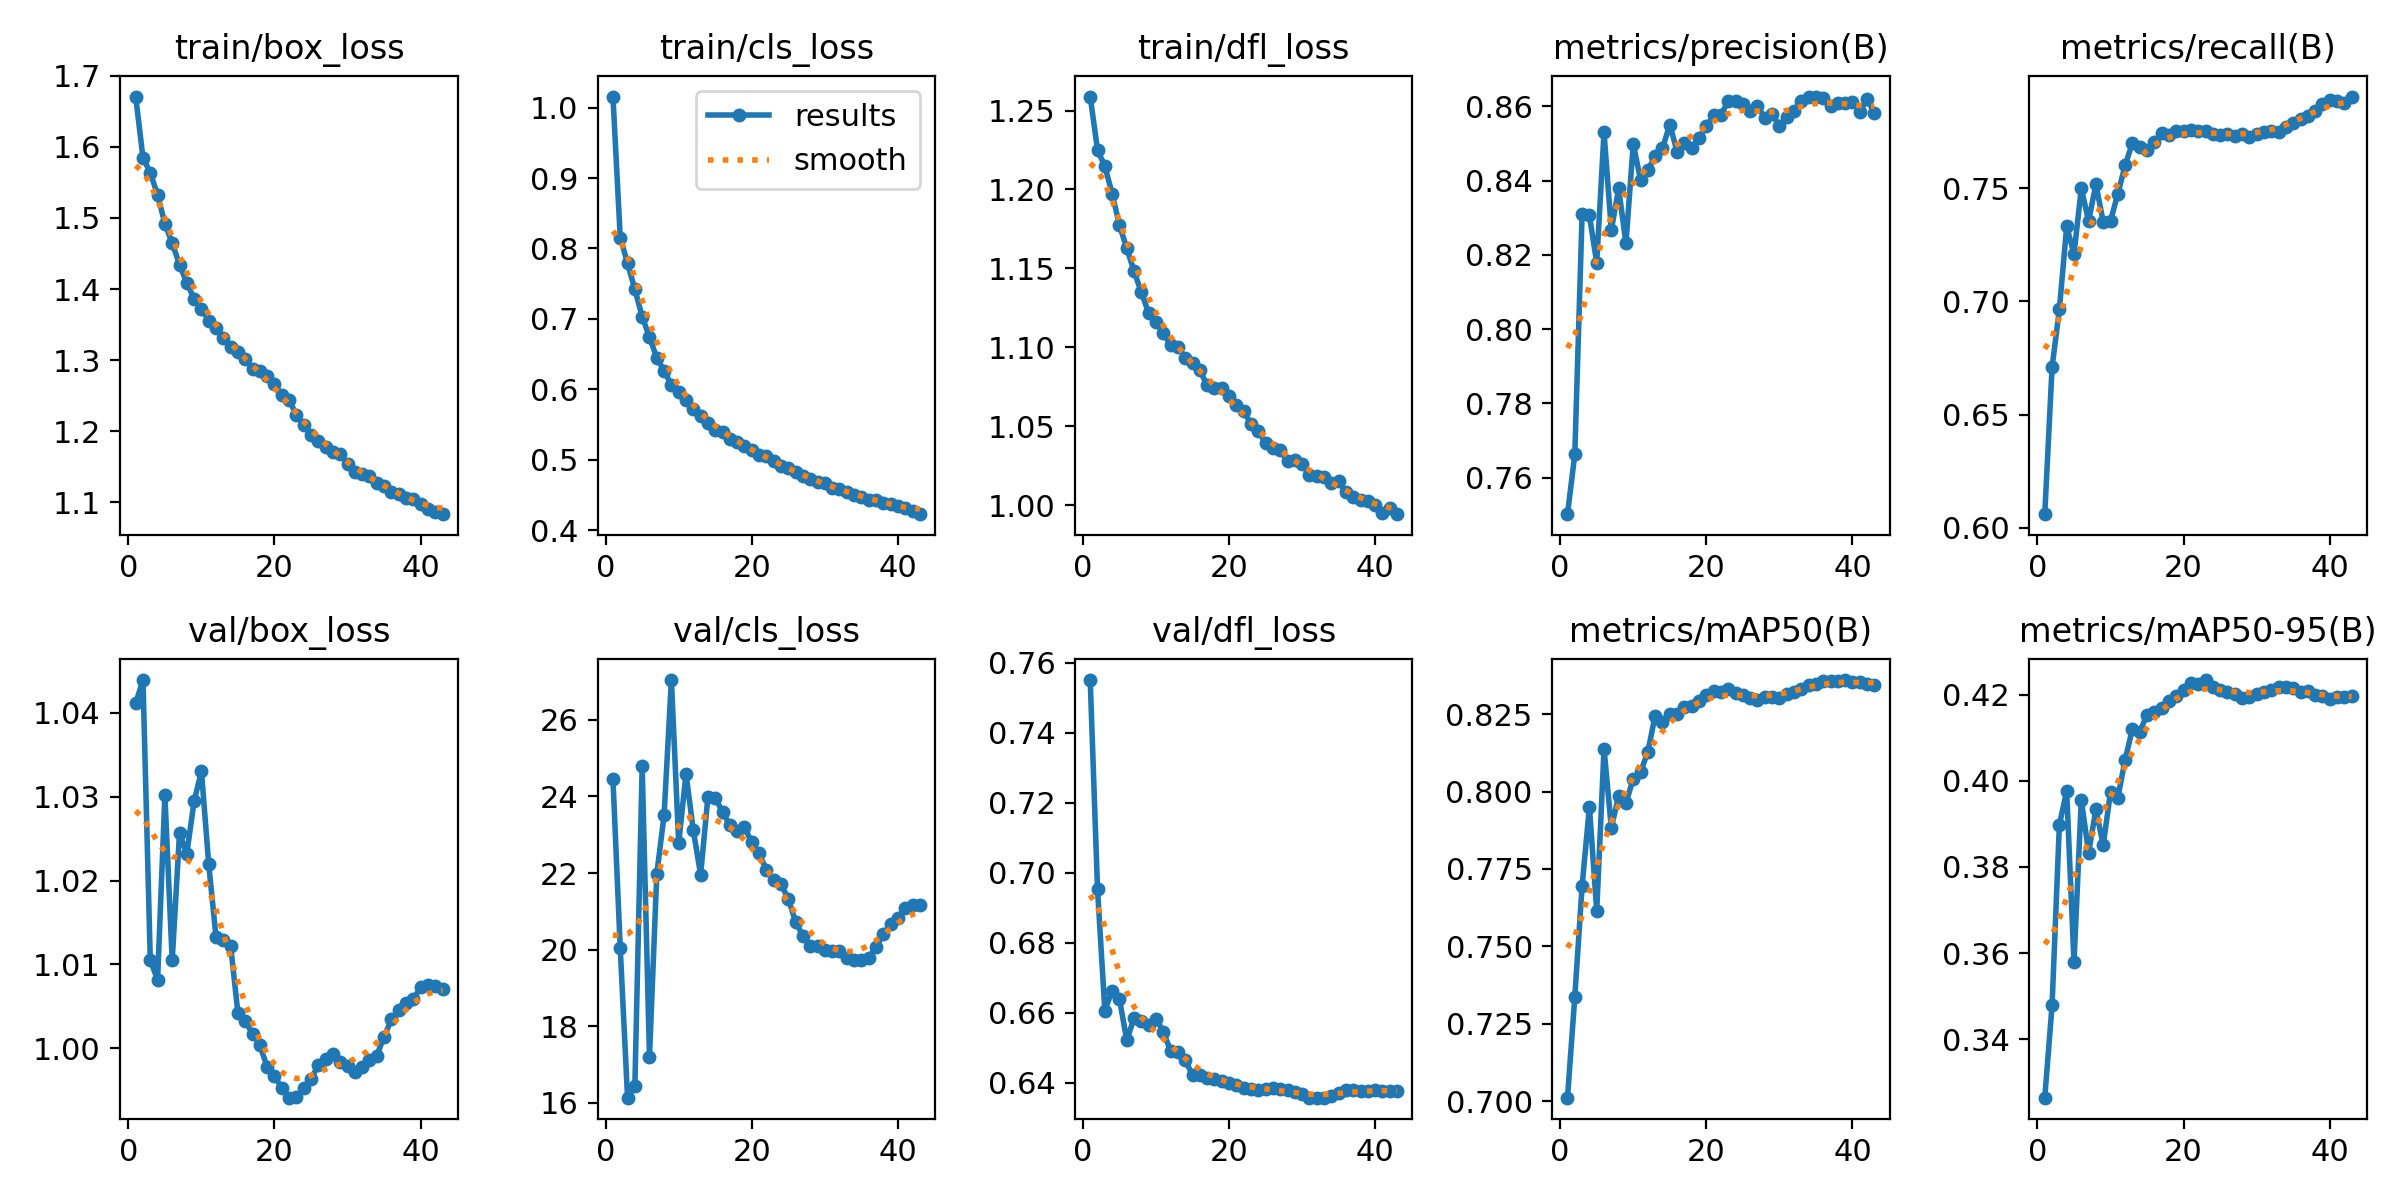
\includegraphics[width=0.95\linewidth]{Figures/Andreas/YOLO/results.png}
    \caption[YOLO results]{YOLOv8n training and validation loss curves over 43 epochs. The box, classification, and distribution focal loss (DFL) all decline consistently during training. A slight increase in validation box loss after epoch 25 indicates marginal overfitting on bounding box regression. The validation classification loss operates at a higher scale than the training classification loss, attributable to the 2,750 background-only images in the validation set actively penalising false detections. The best mAP@0.50 and mAP@0.50:0.95 scores were 0.835 and 0.420 respectively.}
    \label{fig:pYolo_results}
\end{figure}

The best $mAP_{50}$ score was at 0.835 and the $mAP_{50:95}$ was at 0.420 (fig: \ref{tab:yolo_detection_performance}). 

\begin{table}[H]
    \centering
    \caption{YOLOv8N detection performance on the DroneDetectionDataset validation set.}
    \label{tab:yolo_detection_performance}
    \begin{tabular}{lc}
        \toprule
        \textbf{Metric} & \textbf{Value} \\
        \midrule
        Precision           & 0.862 \\
        Recall              & 0.790 \\
        F1 Score            & 0.810 \\
        mAP@0.50            & 0.835 \\
        mAP@0.50:0.95       & 0.420 \\
        Optimal confidence threshold & 0.571 \\
        \bottomrule
    \end{tabular}
\end{table}

The confusion matrix shows a true positive rate of $88\%$ (fig: \ref{fig:Yolo_confusion_matrix}).

\begin{figure}[H]
    \centering
    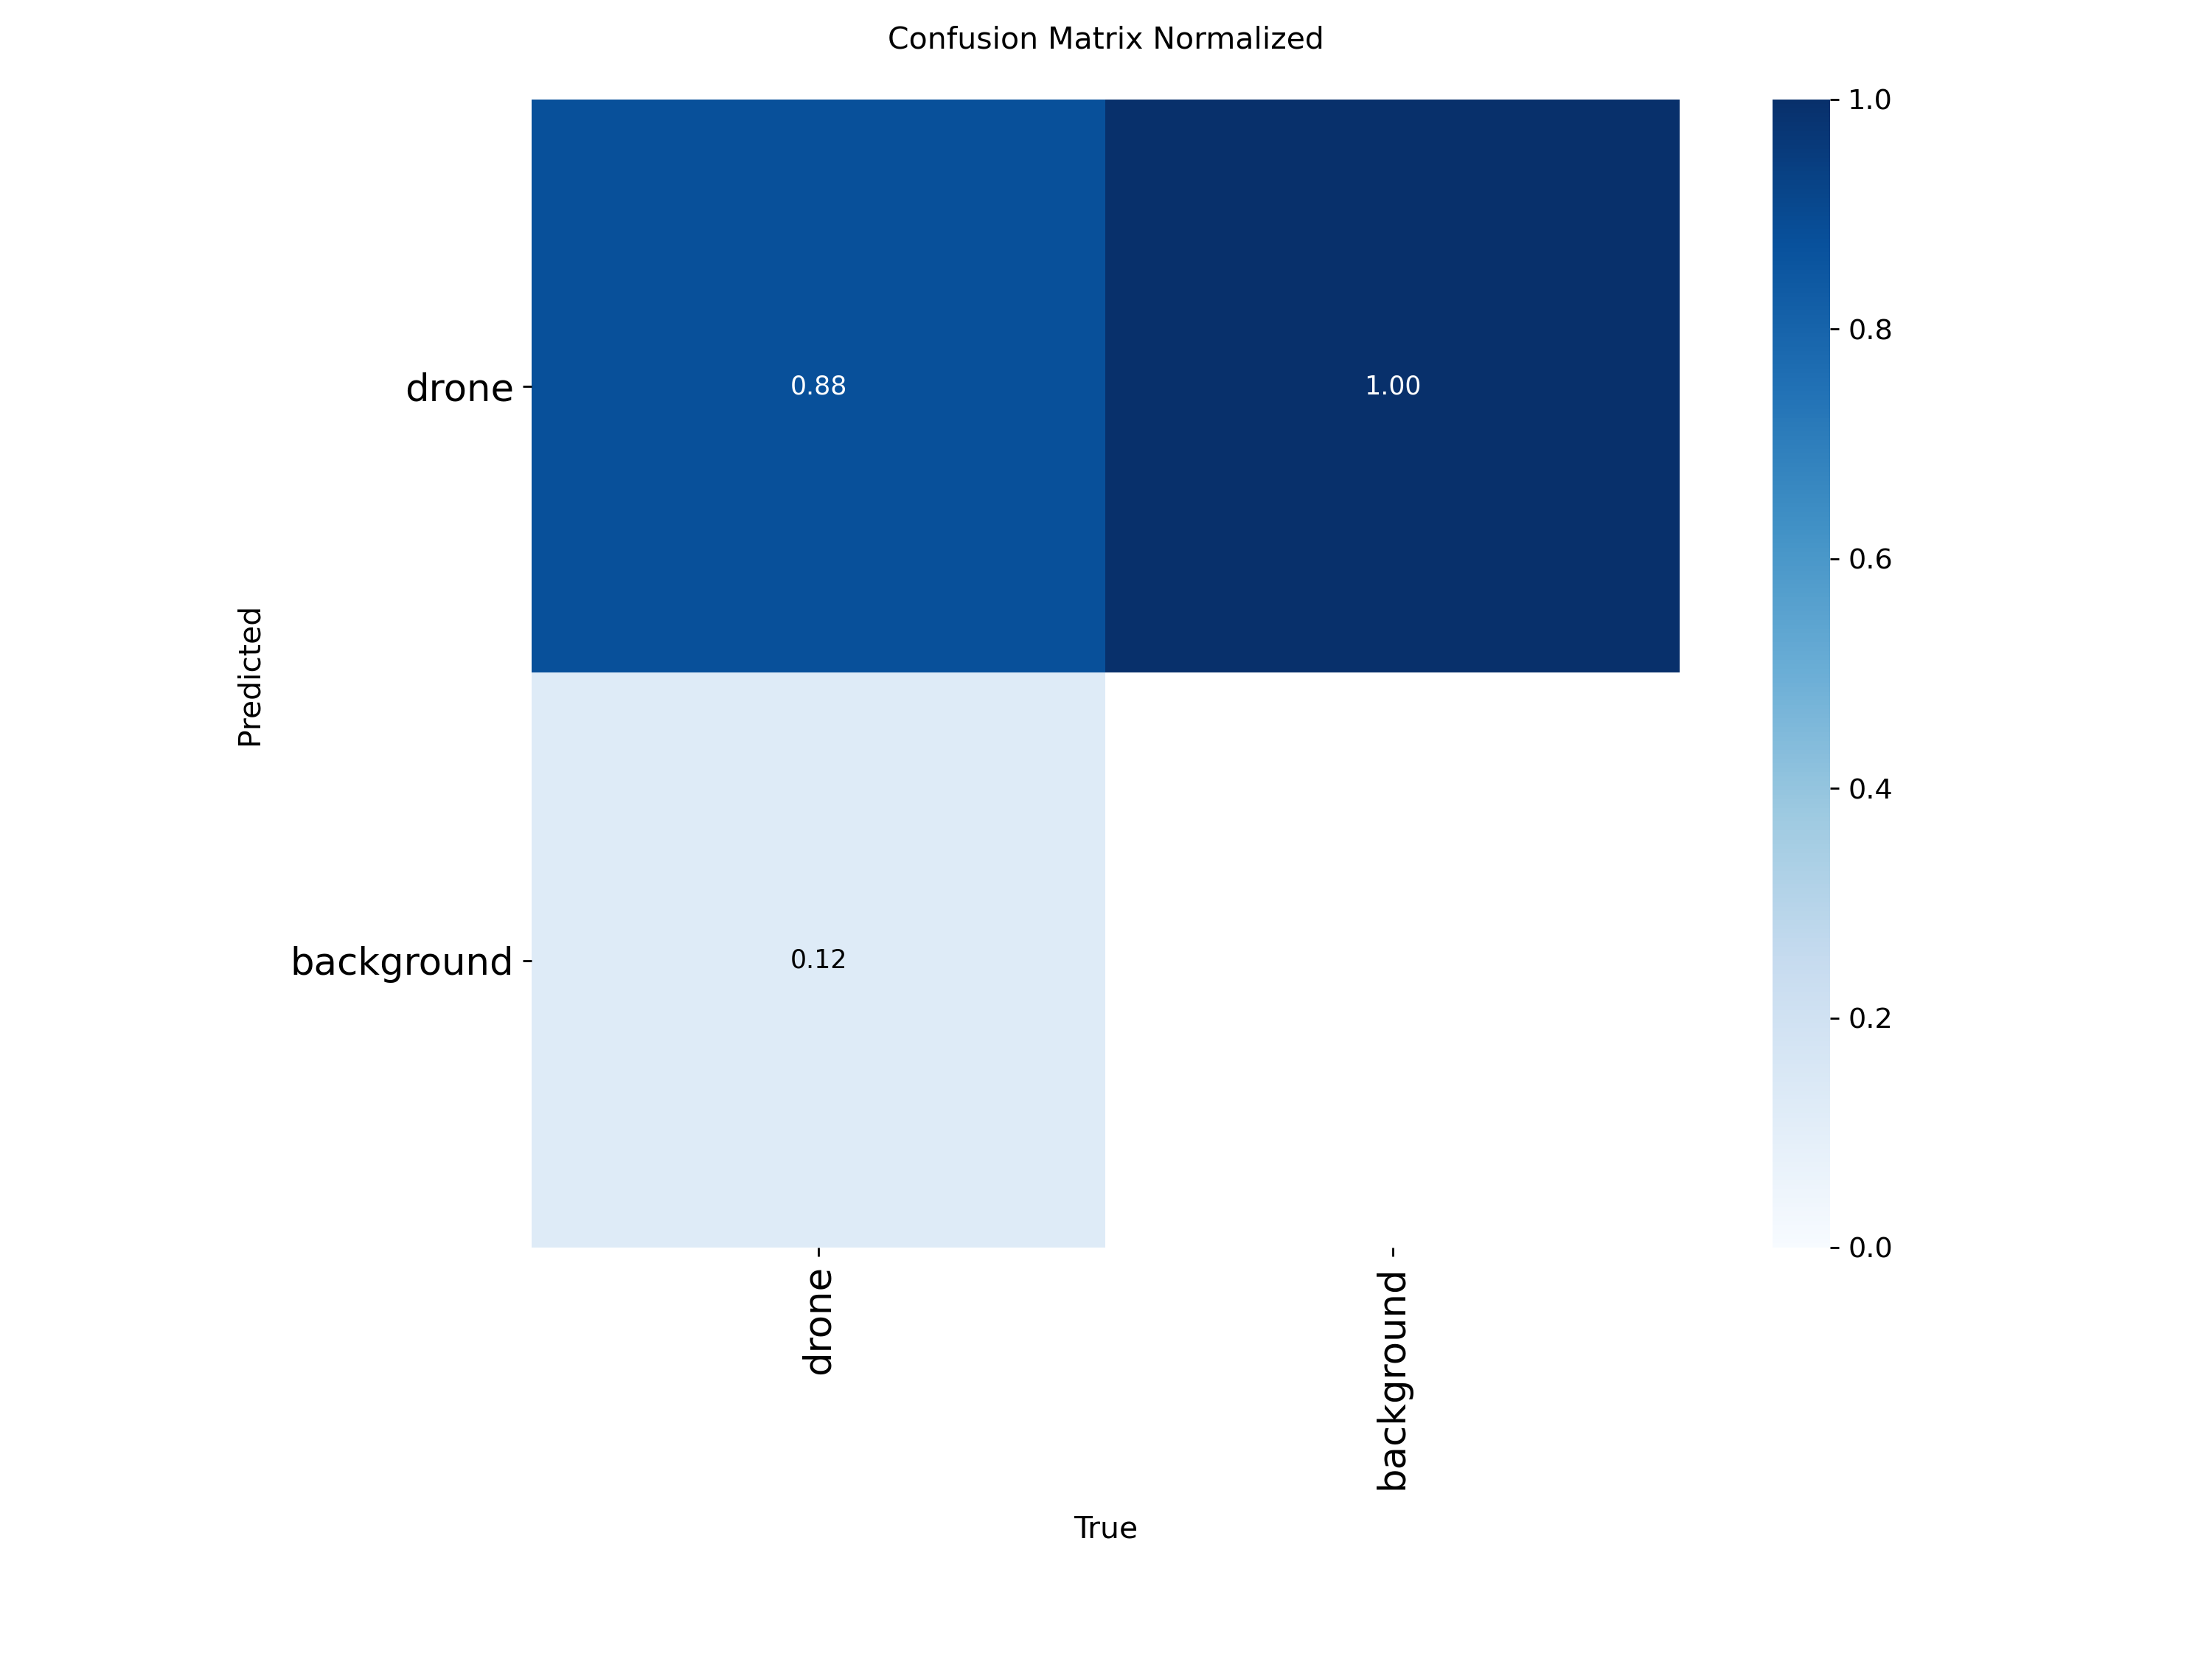
\includegraphics[width=0.95\linewidth]{Figures/Andreas/YOLO/confusion_matrix_normalized.png}
    \caption[YOLO confusion matrix normalized]{Normalised confusion matrix for the YOLOv8n model evaluated on the DroneDetectionDataset validation set. The model achieves a true positive rate of 88\%, with the remaining 12\% of drone instances going undetected. All background instances received a non-zero detection at some confidence level, indicating some false positives, though these are well-controlled at the recommended operating threshold of 0.571}
    \label{fig:Yolo_confusion_matrix}
\end{figure}

The PR curve shows an mAP@0.5 of 0.832. The curve maintains near-perfect precision (>0.95) up to a recall of approximately 0.65, after which precision drops steeply. This indicates the model is highly reliable at moderate recall thresholds but begins trading precision for recall aggressively beyond 0.75 recall. The area under the curve (0.832) confirms strong overall detection performance on a challenging real-world benchmark.(fig: \ref{fig:f1_curve})

The F1 curve peaks at 0.81 at a confidence threshold of 0.571. This is the recommended operating threshold for deployment — detections below this confidence should be discarded. The curve is broad and relatively flat between confidence values of 0.35 and 0.70, meaning the model is robust to moderate threshold adjustments without significant performance loss. Beyond 0.75 confidence the F1 score drops sharply as the model becomes too conservative and misses genuine drones. (fig: \ref{fig:pr_curve}).


\begin{figure}[H]
    \centering
    \begin{subfigure}[b]{0.48\textwidth}
        \centering
        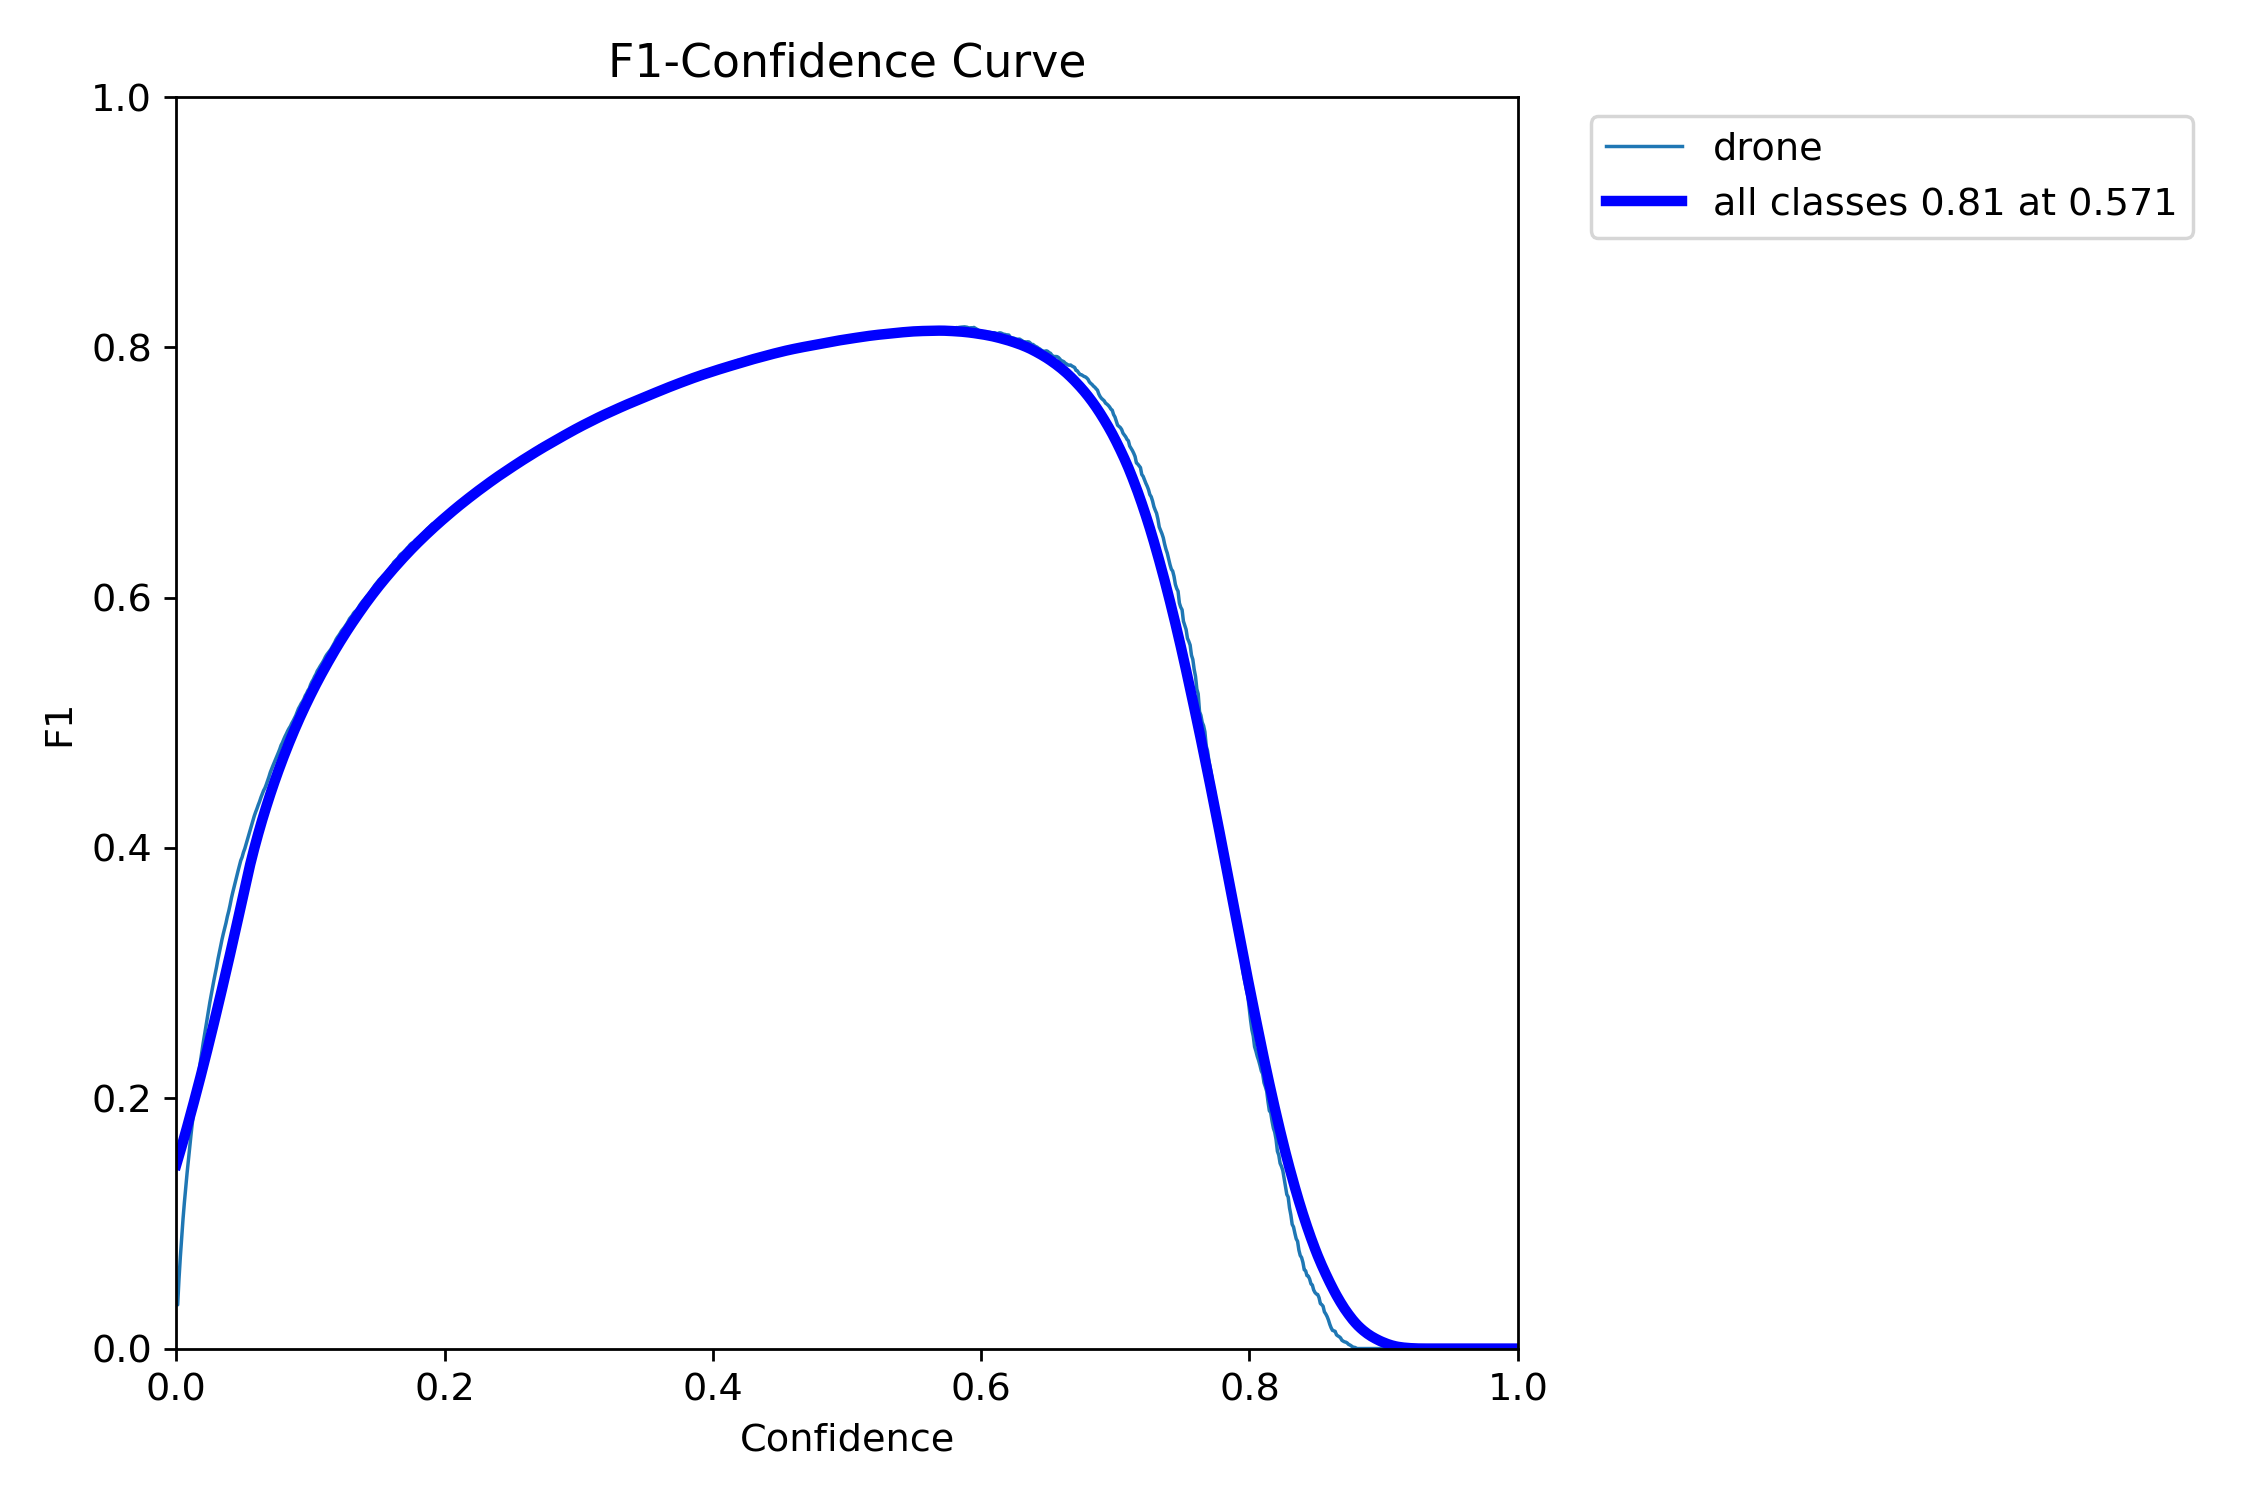
\includegraphics[width=\textwidth]{Figures/Andreas/YOLO/BoxF1_curve.png}
        \caption{F1 score curve}
        \label{fig:f1_curve}
    \end{subfigure}
    \hfill
    \begin{subfigure}[b]{0.48\textwidth}
        \centering
        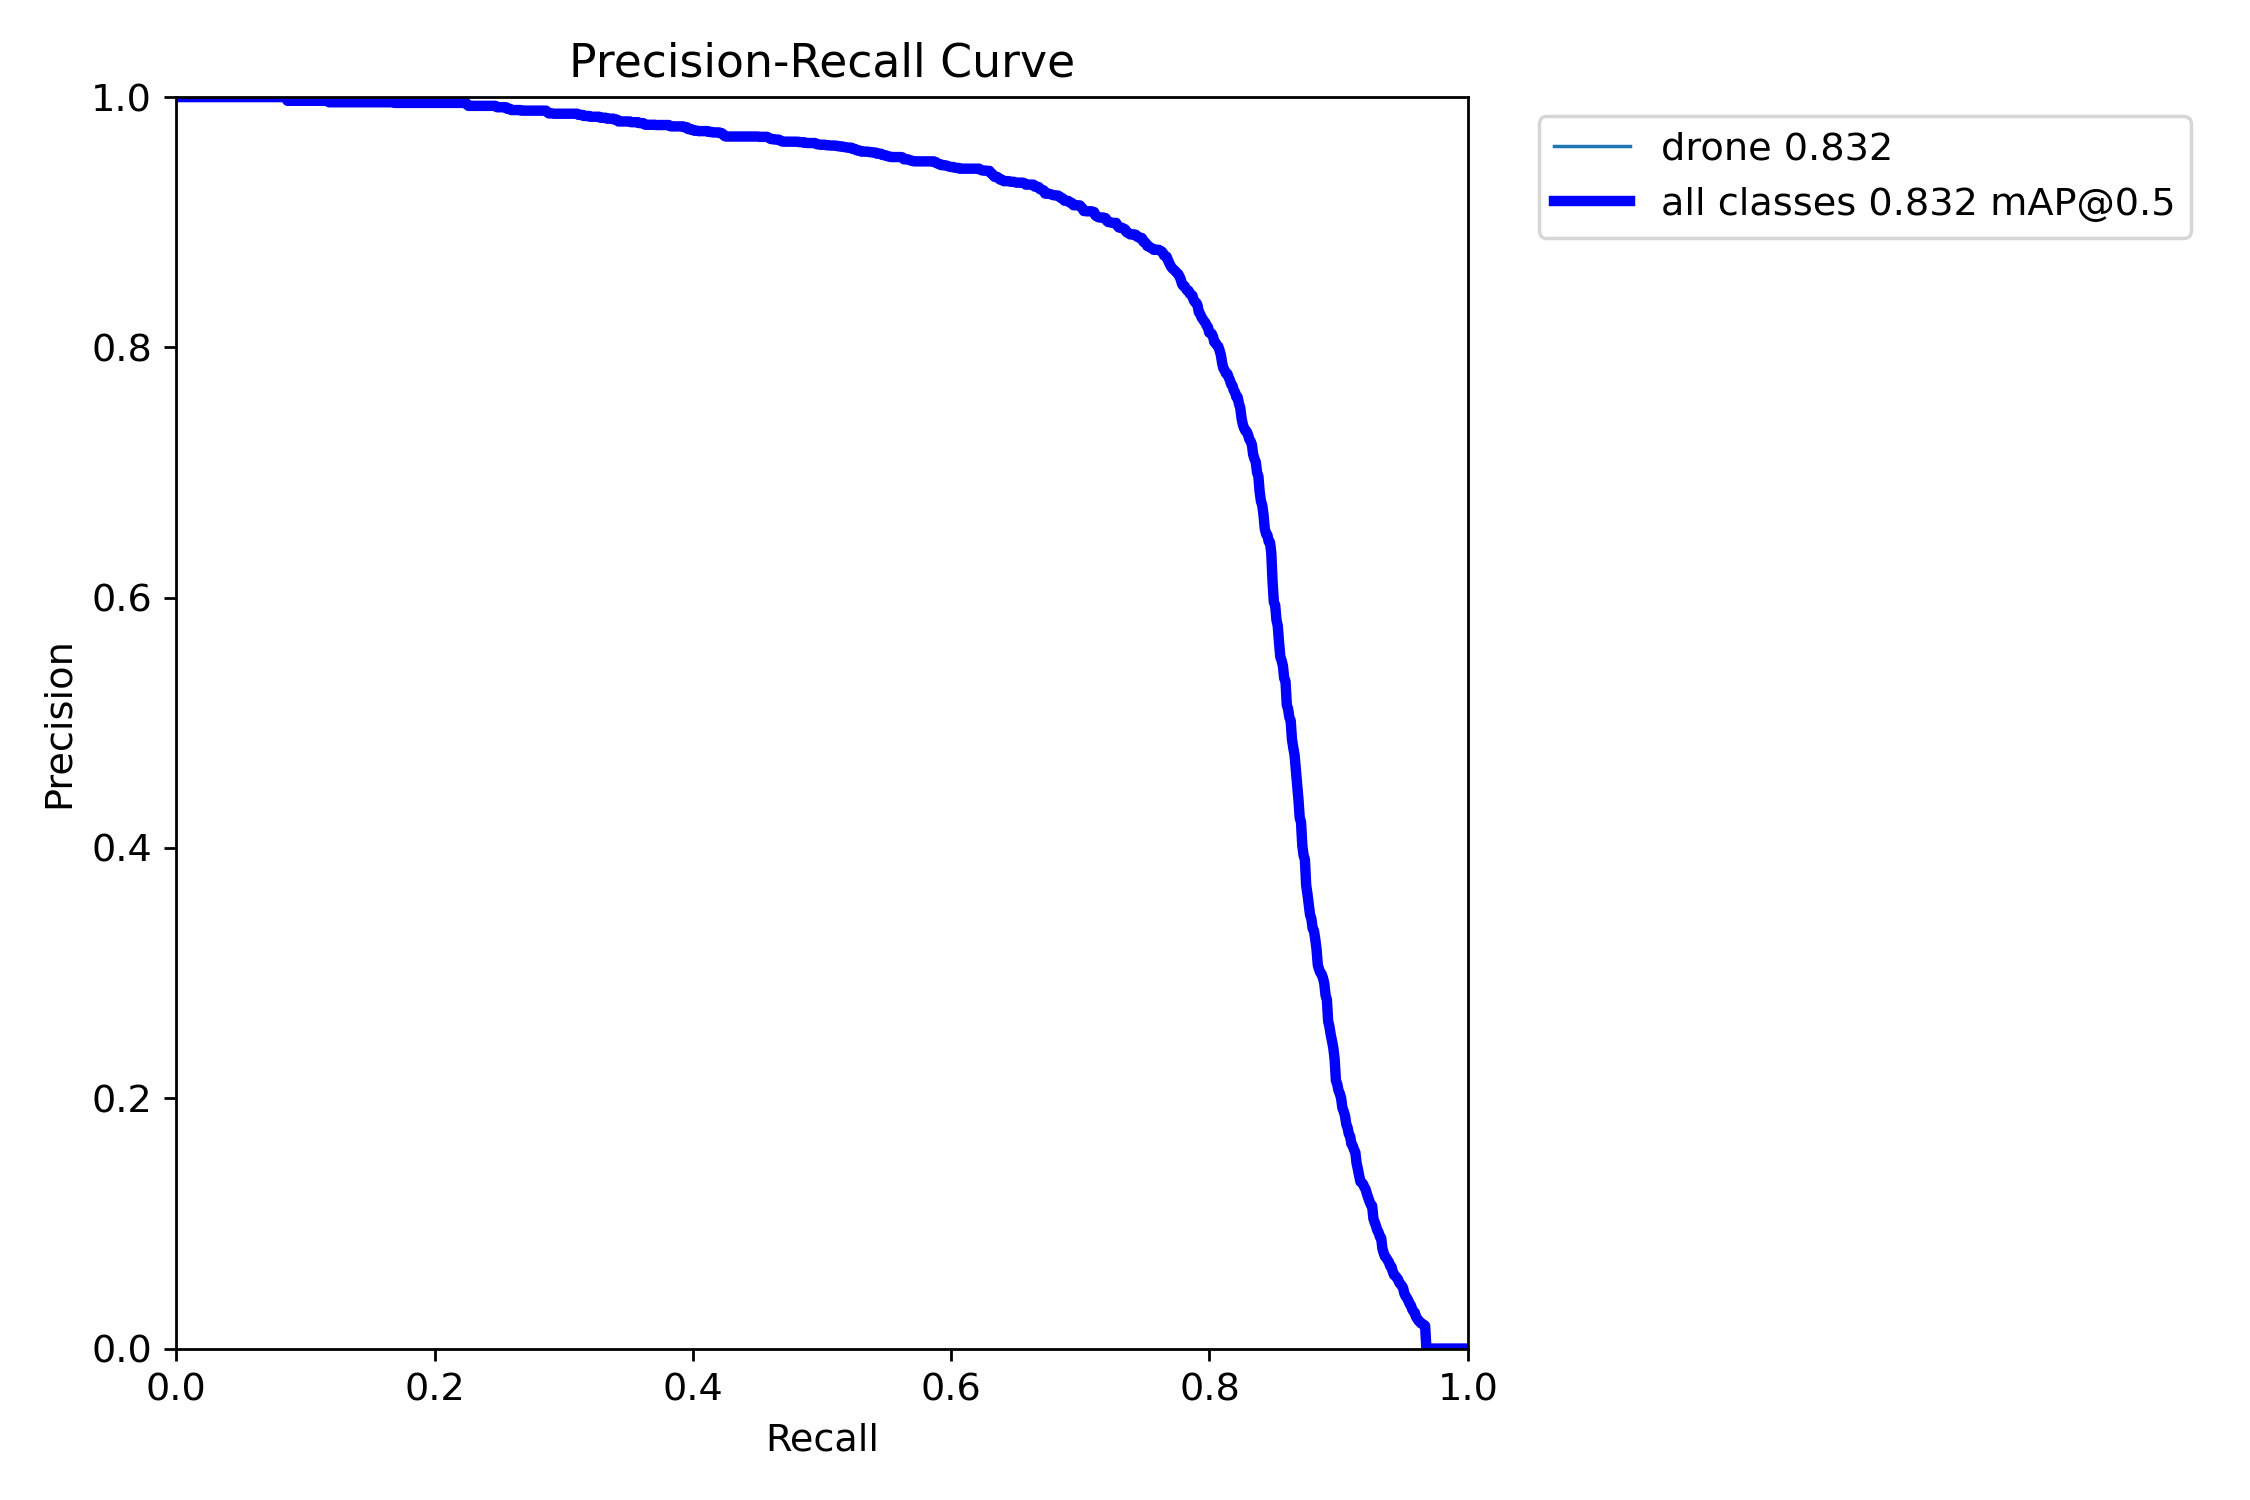
\includegraphics[width=\textwidth]{Figures/Andreas/YOLO/BoxPR_curve.png}
        \caption{Precision-recall curve}
        \label{fig:pr_curve}
    \end{subfigure}
    \caption[F1 and PR curves]{ Precision-recall curve for the YOLOv8n drone detector, showing an mAP@0.50 of 0.832. The model maintains near-perfect precision above 0.95 up to a recall of approximately 0.65, after which precision degrades sharply as the model trades specificity for coverage. (b) F1-confidence curve peaking at 0.81 at a confidence threshold of 0.571, which is used as the recommended deployment threshold. The curve remains broad and relatively flat between confidence values of 0.35 and 0.70, indicating robustness to moderate threshold adjustments.}
    \label{fig:f1_pr_curves}
\end{figure}

\subsection{Video drone detection results}

From the tested videos it was found that overall the YOLO model sucessfully detected the drones in a variety of backgrounds and distances without too many false positives. However in the floureon FPV video (\cite{floureon2017}), it was observed that the model consistently failed to detect the drone when the background was occupied by dark leaved trees (\ref{fig:video_comparison}). 

\begin{figure}[H]
    \centering
    \begin{subfigure}[b]{0.48\textwidth}
        \centering
        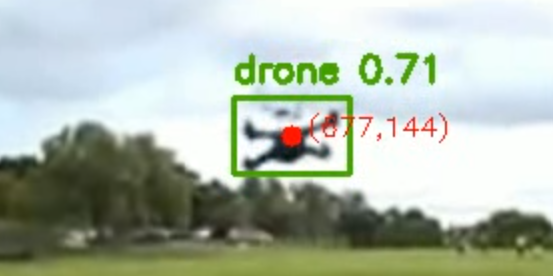
\includegraphics[width=\textwidth]{Figures/Andreas/YOLO/Video_NO_trees.png}
        \caption{Detection without trees}
        \label{fig:video_no_trees}
    \end{subfigure}
    \hfill
    \begin{subfigure}[b]{0.48\textwidth}
        \centering
        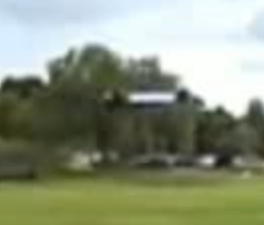
\includegraphics[width=\textwidth]{Figures/Andreas/YOLO/Video_with_trees.png}
        \caption{Detection with trees}
        \label{fig:video_with_trees}
    \end{subfigure}
    \caption[Video detection comparison]{Screenshots taken from one of the videos showcasing the YOLO model.}
    \label{fig:video_comparison}
\end{figure}

The video with the most false positives was found to be the TED talk bideo by Rafaello D'Andrea (\cite{dandrea2016}). In the video there are multiple instances of the YOLO model mistaking a person, as well as a TV (\ref{fig:ted_detections}).

\begin{figure}[H]
    \centering
    \begin{subfigure}[b]{0.48\textwidth}
        \centering
        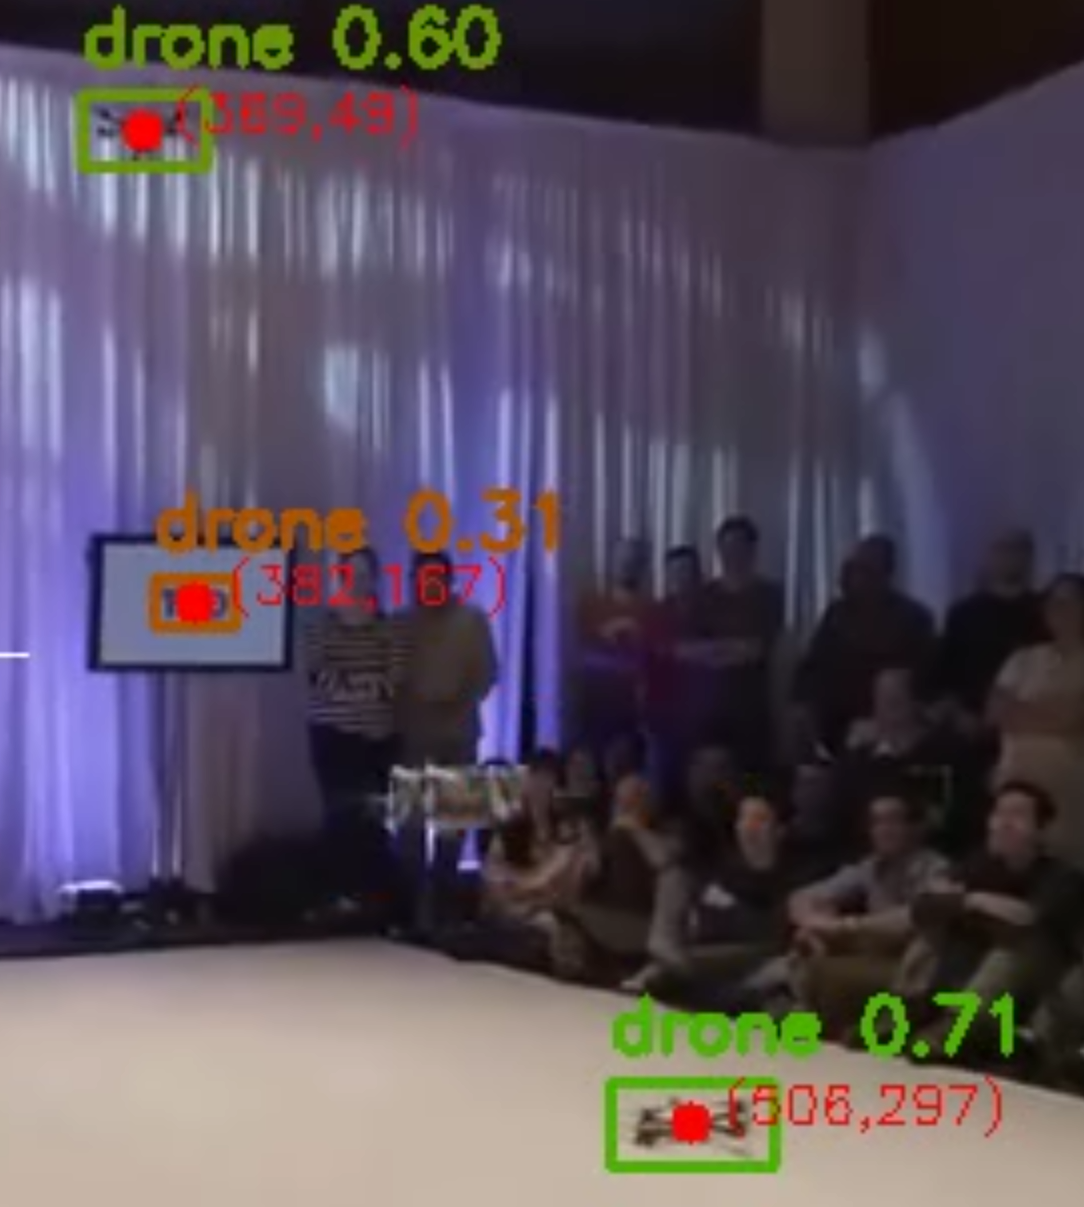
\includegraphics[width=\textwidth]{Figures/Andreas/YOLO/TED_TPandFP.png}
        \caption{True positive and false positive, and a drone thats not detected at all}
        \label{fig:ted_tp_fp}
    \end{subfigure}
    \hfill
    \begin{subfigure}[b]{0.48\textwidth}
        \centering
        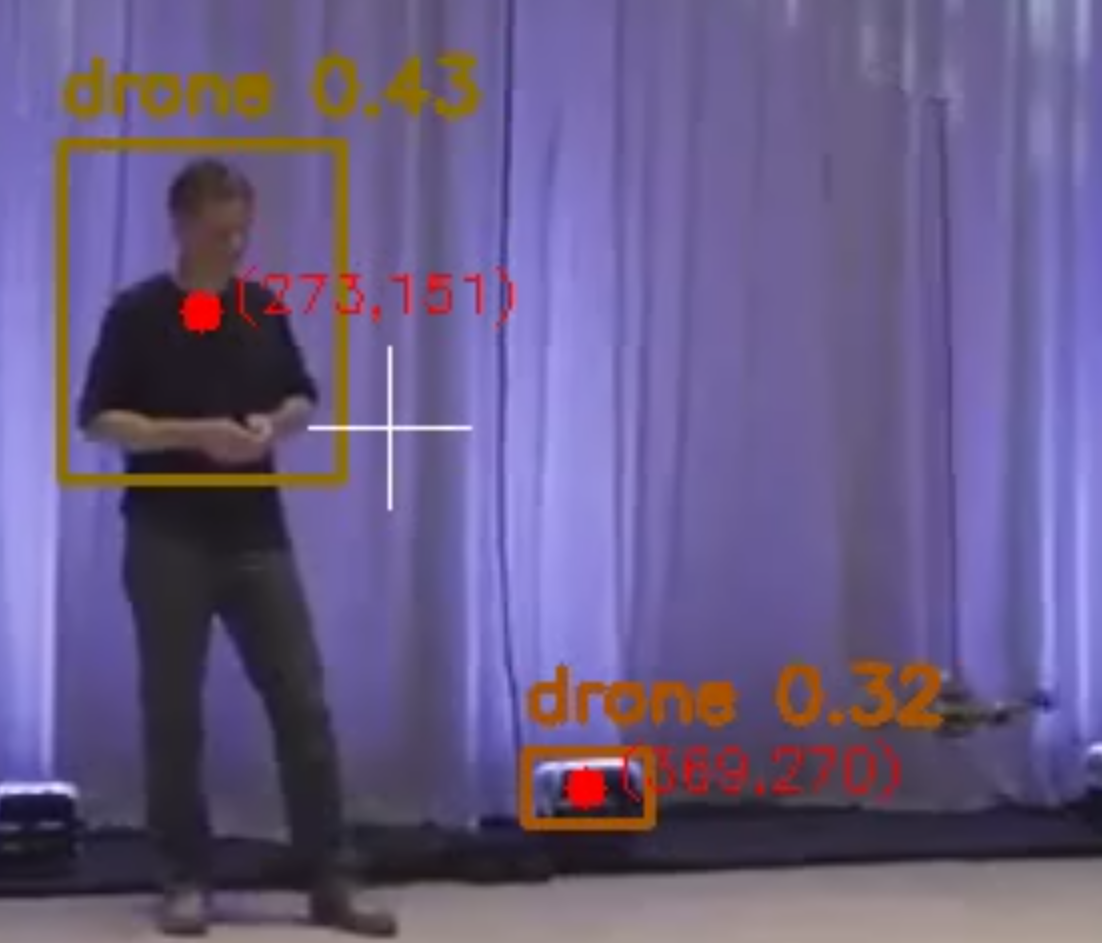
\includegraphics[width=\textwidth]{Figures/Andreas/YOLO/TED_FP_PERSON.png}
        \caption{False positive detection on a person}
        \label{fig:ted_fp_person}
    \end{subfigure}
    \vspace{0.5em}
    \begin{subfigure}[b]{0.6\textwidth}
        \centering
        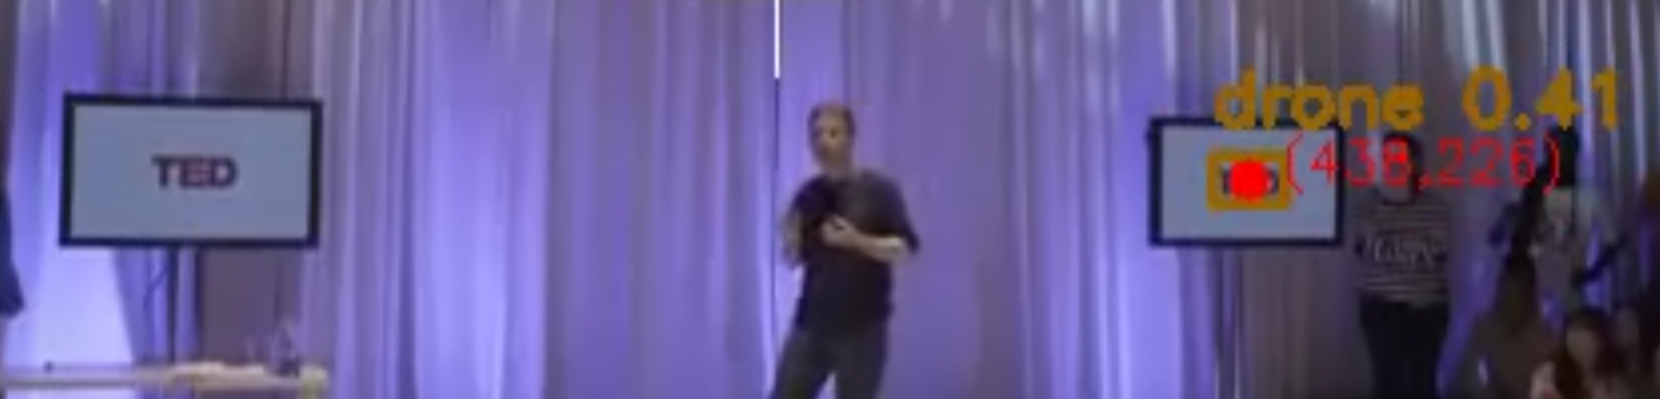
\includegraphics[width=\textwidth]{Figures/Andreas/YOLO/TED_FP.png}
        \caption{False positive detection}
        \label{fig:ted_fp}
    \end{subfigure}
    \caption[TED talk detection examples]{Example detections from the Raffaello D'Andrea TED talk, illustrating false positive detections in a cluttered dark indoor environment (\cite{dandrea2016}).}
    \label{fig:ted_detections}
\end{figure}

The YOLO detection running on the RPI was succesfull in identifying the drone flown in the lab (fig: \ref{fig:Live-lab-test}). The pixel coordinates of the center of the box detection was also successfully sent over via MQTT to the Arduino Nano in the system. 

\begin{figure}[H]
    \centering
    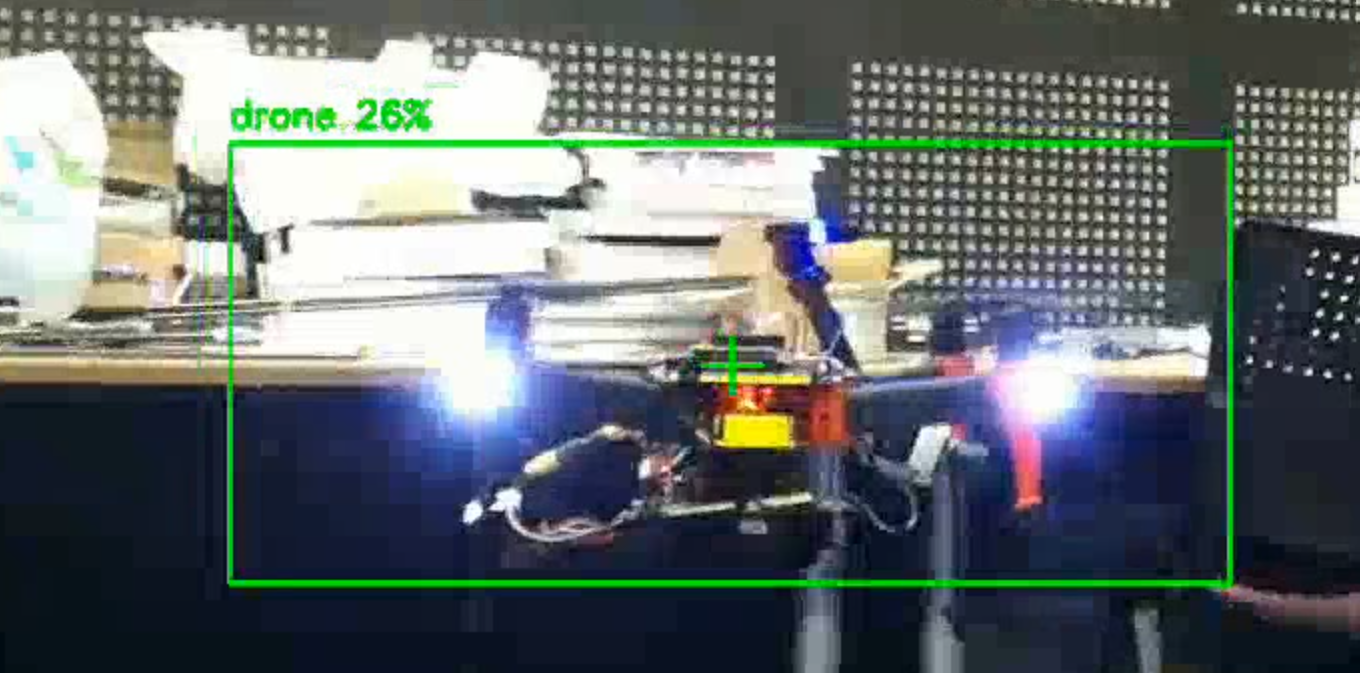
\includegraphics[width=0.5\linewidth]{Figures/Andreas/YOLO/Drone_live_lab.png}
    \caption[YOLO result live test]{Screenshot from the YOLO detection in the live lab test}
    \label{fig:Live-lab-test}
\end{figure}

It should be noted that the live laboratory test was intentionally limited 
in scope. Since the camera tracking functionality was not completed, a 
comprehensive evaluation of the visual detection subsystem was not 
prioritised at this stage. The test was further constrained by the 
laboratory environment itself: the drone could only be flown in close 
proximity to the camera platform due to safety restrictions, the indoor 
setting does not represent the outdoor backgrounds the model was trained 
on, and the drone model available in the laboratory has an irregular 
appearance that differs from the consumer quadcopters dominant in the 
training dataset (\cite{DroneDatasetFinal}). These factors mean the live 
test should be interpreted as a basic proof-of-concept demonstration 
that the inference pipeline functions on the Raspberry Pi hardware, 
rather than a rigorous evaluation of detection performance.


\section{Sound classification result}

The Convolutional Neural Network (CNN) was assessed with TensorFlow’s built-in evaluation function(Figure 4.7.1). On the public dataset the CNN attained an accuracy of 0.80, whereas on the microphone‑array recordings it reached 0.99 accuracy. Moreover, when the microphone‑array data were supplied directly to the trained CNN, the model achieved a perfect score of 49/49 correctly classified instances (Figure 4.7.3a).


\begin{figure}[H]
    \centering
    \begin{subfigure}[a]{0.48\textwidth}
        \centering
        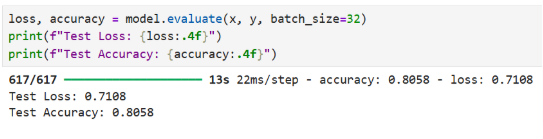
\includegraphics[width=0.95\linewidth]{Figures/Brage/CNNTestPublicData.PNG}
        \caption{CNN evaluation with public datasett(\cite{AudioDatasett})}
        \label{fig:placeholder}
    \end{subfigure}
    \begin{subfigure}[b]{0.48\textwidth}
        \centering
        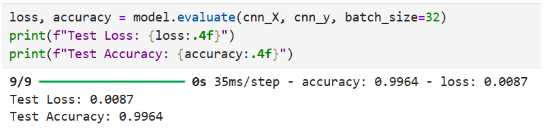
\includegraphics[width=0.95\linewidth]{Figures/Brage/CNNTestMicData.PNG}
        \caption{CNN evaluation with data form microphone array}
        \label{fig:placeholder}
    \end{subfigure}
    \caption{CNN model Tensorflow.evaluate tests}
    \label{fig:placeholder}
\end{figure}

The accumulative model was evaluated in two ways: by using scikit-learn’s k-fold cross-validation (k=5) and by feeding dedicated test sets of sound data directly to the classifier.Using the 5-fold cross-validation, the model achieved a mean accuracy of 0.90(Figure 4.6.2). 

\begin{figure}[H]
    \centering
    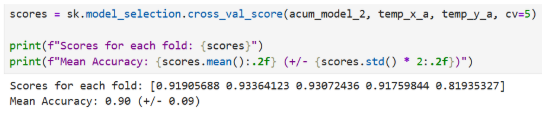
\includegraphics[width=0.9\linewidth]{Figures/Brage/AccumTestCroVal.PNG}
    \caption{Testing of the accumulative model with scikit-learn k-fold cross-validation (k=5)}
    \label{fig:placeholder}
\end{figure}

In contrast when the model was tested with data from the on-board microphone array, The performance collapsed: all predictions were incorrect i.e. the model behaved opposite to expectations(Figure 4.6.3a). When tested directly with a test set composed of the public dataset, which formed the majority of the evaluation data, the accumulative model produced results comparable to those of the CNN model(Figure 4.6.3b).


\begin{figure}[H]
    \centering
    \begin{subfigure}[a]{0.48\textwidth}
        \centering
        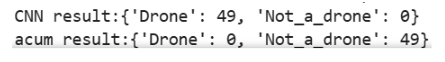
\includegraphics[width=0.9\linewidth]{Figures/Brage/MlTestMicData.PNG}
        \caption{Direct Testing of the CNN model and Accumulative model with data from microphone array}
        \label{fig:placeholder}
    \end{subfigure}
    \begin{subfigure}[b]{0.48\textwidth}
        \centering
        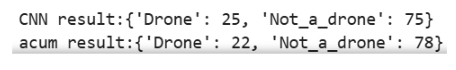
\includegraphics[width=0.9\linewidth]{Figures/Brage/MlTestPublicData.PNG}
        \caption{Direct Testing of the CNN model and Accumulative model with data from public datasett(\cite{AudioDatasett})}
        \label{fig:placeholder}
    \end{subfigure}
    \caption{Direct Testing of the CNN model and Accumulative model}
    \label{fig:placeholder}
\end{figure}

During a live-system test the machine-learning models performed identically to the isolated environment evaluations. The CNN model produced no false-positive or false-negative predictions, whereas the accumulative model consistently outputted the negative class.

The experiment was repeated five times with a drone in flight. In all tests the same outcome was observed, except for a single outlier: the accumulative model detected the drone once out of 30 total prediction iterations(Figure 4.6.4b).

\begin{figure}[H]
    \centering
    \begin{subfigure}[a]{0.48\textwidth}
        \centering
        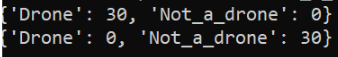
\includegraphics[width=0.85\linewidth]{Figures/Brage/LiveTestStandard.PNG}
        \caption{Standard Machine learning result from live test, upper CNN model, bottom Accumulative model}
        \label{fig:placeholder}
    \end{subfigure}
     \begin{subfigure}[b]{0.48\textwidth}
        \centering
        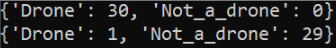
\includegraphics[width=0.85\linewidth]{Figures/Brage/LiveTestOutlier.PNG}
        \caption{Outlier Machine learning result from live test, upper CNN model, bottom Accumulative model}
        \label{fig:placeholder}
    \end{subfigure}
    \caption{Machine learning result from live test}
    \label{fig:placeholder}
\end{figure}

\section{WebServer result}
The webserver code was validated through unit testing using the jest library.The server currently runs at http://localhost:3000 and is not running on a permanent domain. It employs Socket.IO to establish a unidirectional connection with the main Python script that controls the system.
\begin{figure}
    \centering
    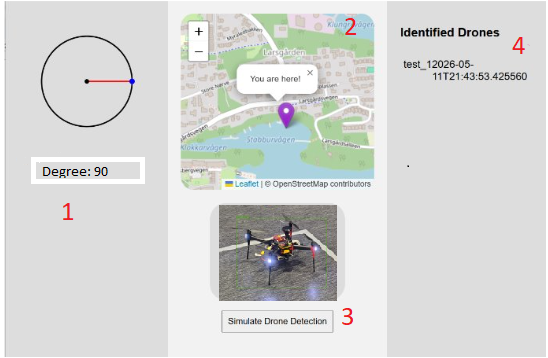
\includegraphics[width=0.75\linewidth]{Figures/Brage/GuiBuildExplain.png}
    \caption{Final build of GUI}
    \label{fig:placeholder}
\end{figure}

Figure 4.7.1 presents the final graphical user interface (GUI). Panel 1 displays a polar diagram with the azimuth degree at which a drone is detected. Panel 2 is an OpenStreetMap view with a marker for the user’s current location. Although the architecture can support drone‑position overlays, the present implementation cannot plot them because distance estimation is not yet available. Panel 3 streams the live camera feed and highlights objects that are recognised as drones. Panel 4 is intended to list identified drones; however, this feature remains under‑developed and currently provides only minimal information.

\subsection{Project Management}
The development process was initially planned according to the Scrum framework .Because team members had varied work schedules and focus on different parts , the actual workflow evolved into a Scrum‑inspired hybrid rather than a strict implementation of Scrum. Mid‑sprint review meetings were held whenever the majority of the team was available. Bi‑weekly sprint‑retrospective meetings were retained, involving the product owner, the project supervisors and the development team.
